% ***************************************************************************************************
%
%	Szablon pracy magisterskiej dla Politechniki Wrocławskiej w wersji dwustronnej.
%	Autor:	Tomasz Strzałka
%
% ***************************************************************************************************

% Styl dwustronny z domyślną wielkością czcionki 10pt oraz oddzieloną stroną tytułową (titlepage).
% Domyślnie rodziały rozpoczynają się na stronie prawej (openright).
\documentclass[oneside]{book}

% ***************************************************************************************************
% Ustawienia języka
% ***************************************************************************************************

% Podstawowe ustawienia języka, według którego formatowany będzie dokument
\usepackage[polish]{babel}

% Pakiet babel dla polskiego języka powoduje konflikt z pakietem amssymb.
% Polecenie '\lll' definiują oba pakiety - porządana jest druga definicja.
\let\lll\undefined

% W przypadku wielojęzykowości ustawia główny język dokumentu
\selectlanguage{polish}

% Kodowanie dokumentu
\usepackage[utf8]{inputenc}

% Dowolny rozmiar czcionek, kodowanie znaków
\usepackage{lmodern}

% Polskie wcięcia akapitów
\usepackage{indentfirst}

% Polskie łamanie wyrazów
\usepackage[plmath]{polski}

% Przecinek w wyrażeniach matematycznych zamiast kropki
\usepackage{icomma}

% Polskie formatowanie typograficzne
\frenchspacing

% Zapewnia liczne usprawnienia wyświetlania i organizacji matematycznych formuł. 
\usepackage{amsmath}

% Wprowadza rozszerzony zestaw symboli m.in. \leadsto
\usepackage{amssymb}

% Dodatkowa, ,,kręcona'' czcionka matematyczna
\usepackage{mathrsfs}

% Dodatkowe wsparcie dla środowiska mathbb, które nie wspiera domyślnie cyfr (\mathbb{})
\usepackage{bbold}

% Fixes/improves amsmath
\usepackage{mathtools}


% ***************************************************************************************************
% Kolory  
% ***************************************************************************************************

% Umożliwia kolorowanie poszczególnych komórek tabeli
\usepackage[table]{xcolor}% http://ctan.org/pkg/

% Umożliwia łatwą zmianę koloru linii w tabeli
\usepackage{tabu}

% Umożliwia rozszerzoną kontrolę nad kolorami.
\usepackage{xcolor}

% Definicje kolorów
\definecolor{lgray}{HTML}{9F9F9F}
\definecolor{dgray}{HTML}{5F5F5F}
% lgray				-	nazwa nowo zdefiniowanego koloru
% HTML				-	model kolorów
% CCCCCC			-	wartość koloru zgodna z modelem

% ***************************************************************************************************
% Algorytmy 
% ***************************************************************************************************

% Udostępnia środowisko do konstruowania pseudokodów
\usepackage[ruled,vlined,linesnumbered,longend,algochapter]{algorithm2e}
% ruled	- poziome kreski na początku i końcu algorytmu, podpis na górze oddzielony również kreską poziomą
% vlined - pionowe kreski łączące początek polecenia z jego końcem
% linesnumbered	- numerowanie kolejnych wierszy algorytmu
% longend - długie końcówki np. ifend, forend itd.
% algochapter - numeracja z rozdziałami

% Zamiana nazwy środowiska z domyślnej "Algorithm X" na "Pseudokod X"
\newenvironment{pseudokod}[1][htb]{
	\renewcommand{\algorithmcfname}{Pseudokod}
	\begin{algorithm}[#1]%
	}{
\end{algorithm}
}

\SetKwComment{Comment}{$\triangleright$\ }{}
\SetKwRepeat{Do}{do}{while}

% Zmiana rozmiaru komentarzy
\newcommand\algcomment[1]{
	\footnotesize{#1}
}

% Ustawienie zadanego stylu dla komentarzy
\SetCommentSty{algcomment}

% Wyśrodkowana tylda
\usepackage{textcomp}%
\newcommand{\textapprox}{\raisebox{0.5ex}{\texttildelow}}

% Listowanie kodów źródłowych
\usepackage{listings} 
\renewcommand{\lstlistingname}{Kod źródłowy} % Polska nazwa listingu

% Definicje pecjalnych znaków, które nie są obsługiwane w środowisku listing
\lstset{literate=
	{ż}{{\.{z}}}1	{ź}{{\'{z}}}1
	{ć}{{\'{c}}}1	{ń}{{\'{n}}}1
	{ą}{{\c a}}1	{ś}{{\'{s}}}1
	{ł}{{\l}}1		{ę}{{\c{e}}}1
	{ó}{{\'{o}}}1	{á}{{\'a}}1
	{é}{{\'e}}1		{í}{{\'i}}1
	{ó}{{\'o}}1		{ú}{{\'u}}1
	{ù}{{\`u}}1		{Á}{{\'A}}1
	{É}{{\'E}}1		{Í}{{\'I}}1
	{Ó}{{\'O}}1		{Ú}{{\'U}}1
	{à}{{\`a}}1		{è}{{\'e}}1
	{ì}{{\`i}}1		{ò}{{\`o}}1
	{ò}{{\`o}}1		{À}{{\`A}}1
	{È}{{\'E}}1		{Ì}{{\`I}}1
	{Ò}{{\`O}}1		{Ò}{{\`O}}1
	{ä}{{\"a}}1		{ë}{{\"e}}1
	{ï}{{\"i}}1		{ö}{{\"o}}1
	{ü}{{\"u}}1		{Ä}{{\"A}}1
	{Ë}{{\"E}}1		{Ï}{{\"I}}1
	{Ö}{{\"O}}1		{Ü}{{\"U}}1
	{â}{{\^a}}1		{ê}{{\^e}}1
	{î}{{\^i}}1		{ô}{{\^o}}1
	{û}{{\^u}}1		{Â}{{\^A}}1
	{Ê}{{\^E}}1		{Î}{{\^I}}1
	{Ô}{{\^O}}1		{Û}{{\^U}}1
	{œ}{{\oe}}1		{Œ}{{\OE}}1
	{æ}{{\ae}}1		{Æ}{{\AE}}1
	{ß}{{\ss}}1		{ç}{{\c c}}1
	{Ç}{{\c C}}1	{ø}{{\o}}1
	{å}{{\r a}}1	{Å}{{\r A}}1
	{€}{{\EUR}}1	{£}{{\pounds}}1
}

% ***************************************************************************************************
% Marginesy 
% ***************************************************************************************************

% Ustawienia rozmiarów stron i ich marginesów
\usepackage[headheight=18pt, top=25mm, bottom=25mm, left=25mm, right=25mm]{geometry}
% headheight		-	wysokość tytułów
% top				-	margines górny
% bottom			-	margines dolny
% left				-	margines lewy
% right				-	margines prawy

% Usunięcie górnego marginesu dla środowisk
\makeatletter
\setlength\@fptop{0\p@}	
\makeatother

% ***************************************************************************************************
% Styl 
% ***************************************************************************************************

% Definiuje środowisko 'titlingpage', które zapewnia pełną kontrolę nad układem strony tytułowej.
\usepackage{titling}


% Umożliwia modyfikowanie stylu spisu treści
\usepackage{tocloft}	

\tocloftpagestyle{tableOfContentStyle}

% Definiowanie własnych stylów nagłówków i/lub stopek
\usepackage{fancyhdr}

% Domyślny styl dla pracy 
\fancypagestyle{custom}{
	\fancyhf{}									% wyczyść stopki i nagłówki
	\fancyhead[RO]{								% Prawy, nieparzysty nagłówek
		\hrulefill \hspace{16pt} \large Rozdział \thechapter
		\put(-472.1, 12.1){%
			\makebox(0,0)[l]{%
				
\includegraphics[width=0.05\textwidth]{pwr-logo}
			}
		}
		\put(-443,5.5){%
			\makebox(0,0)[l]{%
				\small Politechnika Wrocławska
			}
		}
	}
	\fancyhead[LE]{								% Lewy, parzysty nagłówek
		\large Rozdział \thechapter \hspace{16pt} \hrulefill 
		\put(-22, 12.1){%
			\makebox(0,0)[l]{%
				
\includegraphics[width=0.05\textwidth]{wppt-logo}
			}
		}
		\put(-210,5.5){%
			\makebox(0,0)[l]{%
				\small Wydział Podstawowych Problemów Techniki
			}
		}
	}
	\fancyfoot[LE,RO]{							% Stopki
		\thepage
	}
	\renewcommand{\headrulewidth}{0pt}			% Grubość linii w nagłówku
	\renewcommand{\footrulewidth}{0.2pt}		% Grubość linii w stopce
}


% Domyślny styl dla bibliografii
\fancypagestyle{bibliographyStyle}{
	\fancyhf{}									% wyczyść stopki i nagłówki
	\fancyhead[RO]{								% Prawy, nieparzysty nagłówek
		\hrulefill \hspace{16pt} \large Dodatek \thechapter
		\put(-472.1, 12.1){%
			\makebox(0,0)[l]{%
				
\includegraphics[width=0.05\textwidth]{pwr-logo}
			}
		}
		\put(-443,5.5){%
			\makebox(0,0)[l]{%
				\small Politechnika Wrocławska
			}
		}
	}
	\fancyhead[LE]{								% Lewy, parzysty nagłówek
		\large Bibliografia \hspace{16pt} \hrulefill 
		\put(-22, 12.1){%
			\makebox(0,0)[l]{%
				
\includegraphics[width=0.05\textwidth]{wppt-logo}
			}
		}
		\put(-210,5.5){%
			\makebox(0,0)[l]{%
				\small Wydział Podstawowych Problemów Techniki
			}
		}
	}
	\fancyfoot[LE,RO]{							% Stopki
		\thepage
	}
	\renewcommand{\headrulewidth}{0pt}			% Grubość linii w nagłówku
	\renewcommand{\footrulewidth}{0.2pt}		% Grubość linii w stopce
}

% Domyślny styl dla dodatków
\fancypagestyle{appendixStyle}{
	\fancyhf{}									% wyczyść stopki i nagłówki
	\fancyhead[RO]{								% Prawy, nieparzysty nagłówek
		\hrulefill \hspace{16pt} \large Dodatek \thechapter
		\put(-472.1, 12.1){%
			\makebox(0,0)[l]{%
				
\includegraphics[width=0.05\textwidth]{pwr-logo}
			}
		}
		\put(-443,5.5){%
			\makebox(0,0)[l]{%
				\small Politechnika Wrocławska
			}
		}
	}
	\fancyhead[LE]{								% Lewy, parzysty nagłówek
		\large Dodatek \thechapter \hspace{16pt} \hrulefill 
		\put(-22, 12.1){%
			\makebox(0,0)[l]{%
				
\includegraphics[width=0.05\textwidth]{wppt-logo}
			}
		}
		\put(-210,5.5){%
			\makebox(0,0)[l]{%
				\small Wydział Podstawowych Problemów Techniki
			}
		}
	}
	\fancyfoot[LE,RO]{							% Stopki
		\thepage
	}
	\renewcommand{\headrulewidth}{0pt}			% Grubość linii w nagłówku
	\renewcommand{\footrulewidth}{0.2pt}		% Grubość linii w stopce
}

% Osobny styl dla stron zaczynających rozdział/spis treści itd. (domyślnie formatowane jako "plain")
\fancypagestyle{chapterBeginStyle}{
	\fancyhf{}%
	\fancyfoot[LE,RO]{
		\thepage
	}
	\renewcommand{\headrulewidth}{0pt}
	\renewcommand{\footrulewidth}{0.2pt}
}

% Styl dla pozostałych stron spisu treści
\fancypagestyle{tableOfContentStyle}{
	\fancyhf{}%
	\fancyfoot[LE,RO]{
		\thepage
	}
	\renewcommand{\headrulewidth}{0pt}
	\renewcommand{\footrulewidth}{0.2pt}
}

% Formatowanie tytułów rozdziałów i/lub sekcji
\usepackage{titlesec}

% Formatowanie tytułów rozdziałów
\titleformat{\chapter}[hang]					% kształt
{
	\vspace{-10ex}
	\Huge
	\bfseries
}												% formatowanie tekstu modyfikowanego elementu
{}												% etykieta występująca przed tekstem modyfikowanego elementu, niewidoczna w spisie treści
{
	10pt
}												% odstęp formatowanego tytułu od lewego marginesu/etykiety
{
	\Huge
	\bfseries
}												% formatowanie elementów przed modyfikowanym tytułem
[
\vspace{2ex}
%\rule{\textwidth}{0.4pt}
%\vspace{-4ex}
]												% dodatkowe formatowanie stosowane poniżej modyfikowanego tytułu


% Formatowanie tytułów sekcji
\titleformat{\section}[hang]					% kształt
{
	\vspace{2ex}
%	\titlerule\vspace{1ex}
	\Large\bfseries
}												% formatowanie tekstu modyfikowanego elementu
{
	\thesection									% etykieta występująca przed tekstem modyfikowanego elementu, niewidoczna w spisie treści
}
{
	0pt
}												% odstęp formatowanego tytułu od lewego marginesu/etykiety
{
	\Large
	\bfseries
}												% formatowanie elementów przed modyfikowanym tytułem

% ***************************************************************************************************
% Linki
% ***************************************************************************************************

% Umożliwia wstawianie hiperłączy do dokumentu
\usepackage{hyperref}							% Aktywuje linki

\hypersetup{
	colorlinks	=	true,					% Koloruje tekst zamiast tworzyć ramki.
	linkcolor		=	blue,					% Kolory: referencji,
        citecolor		=	blue,					% cytowań,
	urlcolor		=	blue					% hiperlinków.
}

% Do stworzenia hiperłączy zostanie użyta ta sama (same) czcionka co dla reszty dokumentu
\urlstyle{same}




% ***************************************************************************************************
% Linki
% ***************************************************************************************************

% Umożliwia zdefiniowanie własnego stylu wyliczeniowego
\usepackage{enumitem}

% Nowa lista numerowana z trzema poziomami
\newlist{myitemize}{itemize}{3}

% Definicja wyglądu znacznika pierwszego poziomu
\setlist[myitemize,1]{
	label		=	\textbullet,
	leftmargin	=	4mm}

% Definicja wyglądu znacznika drugiego poziomu
\setlist[myitemize,2]{
	label		=	$\diamond$,
	leftmargin	=	8mm}

% Definicja wyglądu znacznika trzeciego poziomu
\setlist[myitemize,3]{
	label		=	$\diamond$,
	leftmargin	=	12mm
}

% ***************************************************************************************************
% Inne pakiety
% ***************************************************************************************************

% Dołączanie rysunków
\usepackage{graphicx}

% Figury i przypisy
\usepackage{subfig}
\usepackage{caption}
%\usepackage{subcaption}

% Umożliwia tworzenie przypisów wewnątrz środowisk
\usepackage{footnote}

% Umożliwia tworzenie struktur katalogów
\usepackage{dirtree}

% Rozciąganie komórek tabeli na wiele wierszy
\usepackage{multirow}

% Precyzyjne obliczenia szerokości/wysokości dowolnego fragmentu wygenerowanego przez LaTeX
\usepackage{calc}
\usepackage{svg}
\usepackage{amsmath}
\usepackage{changepage}
\usepackage{float}
\usepackage{scrextend}
\usepackage{minted}
\usemintedstyle{vs}
\usepackage{array,tabularx,calc}
\usepackage{siunitx}

% \usepackage{algorithm,algpseudocode}

% \makeatletter
% \renewcommand{\fnum@algorithm}{\fname@algorithm}
% \makeatother

\newlength{\conditionwd}
\newenvironment{conditions}[1][gdzie:]
  {%
   #1\tabularx{0.96\textwidth-\widthof{#1}}[t]{
     >{$}l<{$} @{${}-{}$ \vspace*{1em}} X@{}
   }%
  }
  {\endtabularx\\[\belowdisplayskip]}

% ***************************************************************************************************
% Matematyczne skróty
% ***************************************************************************************************

% Skrócony symbol liczb rzeczywistych
\newcommand{\RR}{\mathbb{R}}

% Skrócony symbol liczb naturalnych
\newcommand{\NN}{\mathbb{N}}

% Skrócony symbol liczb wymiernych
\newcommand{\QQ}{\mathbb{Q}}

% Skrócony symbol liczb całkowitych
\newcommand{\ZZ}{\mathbb{Z}}

% Skrócony symbol logicznej implikacji
\newcommand{\IMP}{\rightarrow}

% Skrócony symbol  logicznej równoważności
\newcommand{\IFF}{\leftrightarrow}

% ***************************************************************************************************
% Środowiska
% ***************************************************************************************************

% Środowisko do twierdzeń
\newtheorem{theorem}{Twierdzenie}[chapter]

% Środowisko do lematów
\newtheorem{lemma}{Lemat}[chapter]

% Środowisko do przykładów
\newtheorem{example}{Przykład}[chapter]

% Środowisko do wniosków
\newtheorem{corollary}{Wniosek}[chapter]

% Środowisko do definicji
\newtheorem{definition}{Definicja}[chapter]

% Środowisko do dowodów
\newenvironment{proof}{
	\par\noindent \textbf{Dowód.}
}{
\begin{flushright}
	\vspace*{-6mm}\mbox{$\blacklozenge$}
\end{flushright}
}

% Środowisko do uwag
\newenvironment{remark}{
	\bigskip \par\noindent \small \textbf{Uwaga.}
}{
\begin{small}
	\vspace*{4mm}
\end{small}
}

% ***************************************************************************************************
% Słownik
% ***************************************************************************************************

% Prawidłowe dzielenie wyrazów
\hyphenation{wszy-stkich ko-lu-mnę każ-da od-leg-łość
	dzie-dzi-ny dzie-dzi-na rów-nych rów-ny
	pole-ga zmie-nna pa-ra-met-rów wzo-rem po-cho-dzi
	o-trzy-ma wte-dy wa-run-ko-wych lo-gicz-nie
	skreś-la-na skreś-la-ną cał-ko-wi-tych wzo-rów po-rzą-dek po-rząd-kiem
	przy-kład pod-zbio-rów po-mię-dzy re-pre-zen-to-wa-ne
	rów-no-waż-ne bi-blio-te-kach wy-pro-wa-dza ma-te-ria-łów
	prze-ka-za-nym skoń-czo-nym moż-esz na-tu-ral-na cią-gu tab-li-cy
	prze-ka-za-nej od-po-wied-nio}

% ***************************************************************************************************
% Dokument
% ***************************************************************************************************

\frontmatter

\begin{document}
	\begin{titlingpage}
		\vspace*{\fill}
		\begin{center}
			\begin{picture}(300,510)
				\put(11,520){\makebox(0,0)[l]{\large \textsc{Wydział Podstawowych Problemów Techniki}}}
				\put(11,500){\makebox(0,0)[l]{\large \textsc{Politechnika Wrocławska}}}
% Tytuł pracy
				\put(80,320){\Huge \textsc{Uczenie maszynowe -}}
				\put(80,280){\Huge \textsc{optymalizacja,}}
				\put(80,240){\Huge \textsc{determinizm}}
% Autor pracy
				\put(90,200){\makebox(0,0)[l]{\large \textsc{Adam Jochna}}}
				\put(90,180){\makebox(0,0)[l]{\large \textsc{245681}}}

				\put(200,100){\makebox(0,0)[l]{\large Praca inżynierska napisana}}
				\put(200,80){\makebox(0,0)[l]{\large pod kierunkiem}}
% dane promotora
				\put(200,60){\makebox(0,0)[l]{\large dr hab. inż. Łukasza Krzywieckiego}}
				
				\put(115,-70){
\includegraphics[width=0.15\textwidth]{pwr}}
				\put(106,-80){\makebox(0,0)[bl]{\large \textsc{Wrocław 2021}}}
			\end{picture}
		\end{center}	
		\vspace*{\fill}
	\end{titlingpage}
	
        \cleardoublepage
		
	\pagenumbering{Roman}
	\pagestyle{tableOfContentStyle}
	\tableofcontents
	\cleardoublepage
		
	% ***************************************************************************************************
	% Wstęp
	% ***************************************************************************************************
	
	\pagestyle{custom}
	\mainmatter
	
	% ***************************************************************************************************
	% Rodziały
	% ***************************************************************************************************

	\chapter*{Wstęp}
\addcontentsline{toc}{chapter}{Wstęp}

\thispagestyle{chapterBeginStyle}

\section*{Cel pracy}

Celem pracy inżynierskiej jest skonstruowanie modelu pozwalającego przewidzieć położenie pojazdu uczestniczącego w ruchu drogowym. Formalnie problem ten polega na znalezieniu funkcji $f$, która przekształca dane wejściowe na predykcje. Określenie funkcja $f$ i model predykcyjny jest w kontekście tej pracy tożsame.

\section*{Zakres pracy}

\noindent Zakres pracy obejmuje następujące zagadnienia:

\begin{itemize}
    \setlength{\itemsep}{1pt}
    \setlength{\parskip}{0pt}
    \setlength{\parsep}{0pt}
    \item Opis zbioru dotyczącego ruchu drogowego
    \item Wybór optymalnego sposobu przetwarzanie zbioru
    \item Zaproponowanie architektur modeli predykcyjnych i zaprogramowanie ich
    \item Wytrenowanie kilku sieci neuronowych
    \item Wybór optymalnego modelu predykcyjnego ruchu agentów
    \item Porównanie modeli opartych o głębokie sieci neuronowe z prostymi modelami kinetycznymi
    \item Porównanie metod łączenia wyników wielu modeli predykcyjnych
\end{itemize}

\section*{Zawartość pracy}

\noindent Rozdziały pracy wraz z opisem zawartości:
\begin{enumerate}[label*=\arabic*.]
    \setlength{\itemsep}{1pt}
    \setlength{\parskip}{0pt}
    \setlength{\parsep}{0pt}
    \item \textbf{Analiza problemu} - Opis problemu, klasyfikacja typu problemu, opis struktury zbioru oraz sposobów na wczytywanie jego elementów.
    \item \textbf{Rasteryzacja sceny} - Opis możliwych sposobów uzyskania informacji na temat scen w formie obrazu. Opis rasteryzatora z biblioteki \texttt{l5kit} oraz rasteryzatora \texttt{CenterLines}. Pokazanie różnic tych rasteryzatorów. Opis algorytmów, jakie są wykorzystywane przez te rasteryzatory.
    \item \textbf{Funkcja kosztu} - Opis funkcji kosztu, pokazanie jakie są jej składowe oraz wizualizacja wartości tej funkcji dla różnych danych wejściowych.
    \item \textbf{Naiwna metoda rozwiązania problemu} - Przedstawienie sposobu na przewidywanie ruchu agenta \texttt{EGO} za pomocą prostego modelu wykorzystującego pewne proste założenia na temat ruchu agentów.
    \item \textbf{Głębokie sieci neuronowe} - Przedstawienie architektury sieci neuronowych pozwalających przewidywać ruch agentów, z użyciem obrazu \texttt{BEV} (widok z góry na scenę).
    \item \textbf{Proces trenowania sieci neuronowych} - Opis procesu trenowania oraz tego jak efektywnie trenować kilka sieci równolegle. Opis strategii walidacji procesu trenowania.
    \item \textbf{Agregacja modeli} - Opis sposobów jakimi można połączyć wyniki kilku modeli. Opis tego w jaki sposób takie podejście wpływa na jakość i szybkość predykcji.
    \item \textbf{Opis ostatecznego rozwiązania} - Opis najlepszego sposobu na uzyskanie predykcji. Opis parametrów sieci oraz analiza przypadków w których sieć popełnia błędy.
    \item \textbf{Determinizm procesu trenowania} - Opis sposobu uzyskania powtarzalności procesu trenowania.
\end{enumerate}
	\cleardoublepage

	\chapter{Analiza problemu}
\thispagestyle{chapterBeginStyle}
\label{rozdzial1}

\section{Ogólny opis problemu}

\noindent Definicje użyte w opisie modelu i w dalszej części pracy:
\begin{itemize}
    \setlength{\itemsep}{1pt}
    \setlength{\parskip}{0pt}
    \setlength{\parsep}{0pt}
    \item agent - uczestnik ruchu drogowego (pieszy, rowerzysta lub pojazd)
    \item scena - otoczenie pewnego agenta, zawierające drogi, pasy ruchu, agentów i światła
    \item agent \texttt{EGO} - agent, którego ruch jest przewidywany (wybrany agent ze sceny)
    \item chwila $t$ - wybrany punkt na osi czasu podany w sekundach czasu uniksowego
    \item pozycje wejściowe w chwili $t$ - pozycje wybranego agenta które zostały zapisane przed chwilą $t$
    \item pozycje wyjściowe w chwili $t$ - pozycje wybranego agenta które zostały zapisane po chwili $t$
\end{itemize}

Problem poddany analizie w tej pracy można przedstawić następująco. Mając dane wejściowe, czyli: pozycje granic dróg, kierunki jazdy, jakie obowiązują na drogach, pozycje świateł, kolory świateł, pozycje agentów (piesi, rowerzyści, pojazdy) w ustalonych chwilach \mbox{$[t, t-0.1, ... , t-1.0]$}, trzeba wykorzystać te informacje do przewidzenia pozycji wybranego agenta (niekoniecznie pojazdu, może być np. pieszy) możliwie dokładnie w chwilach \mbox{$[t+0.1, t+0.2, ... , t+5.0]$}.

\begin{figure}[htbp]
    \centering
    \subfloat[\centering Scena przed predykcją]{{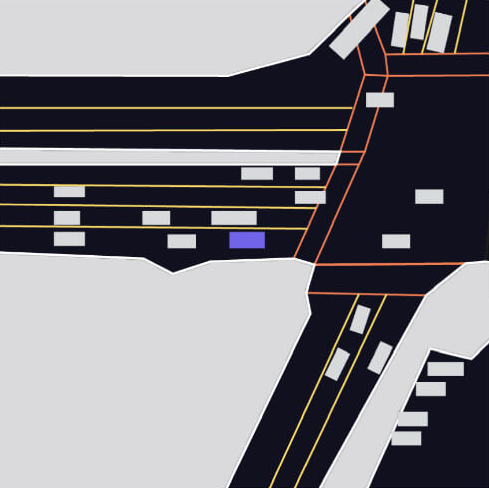
\includegraphics[width=0.47\linewidth]{pred_before.png} }}
    \qquad
    \subfloat[\centering Scena po predykcji]{{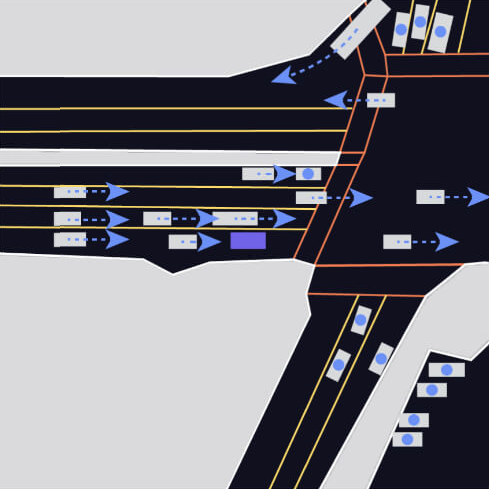
\includegraphics[width=0.47\linewidth]{pred_after.png} }}
    \caption{Wizualizacja problemu}
\end{figure}

\newpage

\section{Formalny opis problemu}

\noindent Problem poruszony w tej pracy polega na skonstruowaniu modelu predykcyjnego (funkcji $f$):
\begin{equation}
f(E_{t}, S_{t}, L_{t}) = ((V_{t}^{0}, P_{t}^{0}), (V_{t}^{1}, P_{t}^{1}), (V_{t}^{2}, P_{t}^{2}))
\end{equation}

\begin{conditions}
     E_{t}     &  Pozycje wejściowe agenta \texttt{EGO}, lista 11 pozycji \mbox{$[(x_{0},y_{0}), (x_{1},y_{1}), ... , (x_{10},y_{10})]$}, które zapisane są w odstępach 0.1 sekundy i dotyczą chwil \mbox{$[t, t-0.1, ... , t-1.0]$}\\
     S_{t}     &  Pozycje wejściowe agentów innych niż agent \texttt{EGO} (agenci są wybierani spośród otoczenia agenta \texttt{EGO}), jest to macierz w której każdy wiersz odpowiada wybranemu agentowi z otoczenia (innemu niż \texttt{EGO}), a każda kolumna odpowiada wybranej chwili w czasie. Komórka $S_{t}[i, j]$ zawiera współrzędne $(x, y)$ i-tego agenta  w chwili $t-j*0.1$ dla $j \in \{0, 1, ... , 10\}$.\\
     L_{t}     &  Lista wszystkich pasów ruchu i ich statusu przejezdności w chwili $t$. Każdy element to słownik z atrybutami \texttt{xyz\_left}, \texttt{xyz\_right}, \texttt{lights}. Atrybuty \texttt{xyz\_left}, \texttt{xyz\_right} zawierają listy współrzędnych węzłów interpolujących odpowiednio lewą i prawą krawędź pasa. Atrybut \texttt{lights} zawiera status przejezdności pasa. Wartość \texttt{'default'} (brak świateł) lub \texttt{'green'} oznacza, że pas jest przejezdny. Wartość \texttt{'red'} oznacza, że pas nie jest przejezdny.\\
     V_{t}^{k}     &  Dla $k \in \{0, 1, 2\}$ $V_{t}^{k}$ zawiera k-tą predykcję trajektorii ruchu agenta. Model nie musi przewidywać najbardziej prawdopodobnej trajektorii ruchu. Model może przewidzieć 3 trajektorie i każdej z nich przypisać prawdopodobieństwo z jaką dana trajektoria wystąpi. Lista $V_{t}^{k}$ zawiera 50 pozycji \mbox{$[(x_{0},y_{0}), (x_{1},y_{1}), ... , (x_{49},y_{49})]$}, które dotyczą chwil \mbox{$[t+0.1, t+0.2, ... , t+5.0]$}.\\
     P_{t}^{k}     &  Dla $k \in \{0, 1, 2\}$ $P_{t}^{k}$ zawiera przewidywane prawdopodobieństwo z jakim wystąpi ruch pojazdu po k-tej trajektorii (zostanie zrealizowana trasa zawarta w $V_{t}^{k}$). Zakłada się, że suma tych prawdopodobieństw wynosi $1$.
\end{conditions}

\section{Typ problemu}

Problem przewidywania pozycji wyjściowych agenta ruchu drogowego w chwili $t$, mając do dyspozycji pozycje wejściowe w chwili t, można rozważać jako problem uczenia nadzorowanego, gdzie na wejście modelu przekazuje się wszystkie dostępne informacje na temat sceny ruchu, a na wyjściu modelu otrzymuje się przewidywane trajektorie wybranego agenta ze sceny w ustalonym przedziale czasowym.

\section{Charakter problemu}

Problem przewidywania przyszłych pozycji obiektów uczestniczących w ruchu drogowym ma charakter praktyczny. Analizowany problem został zaczerpnięty z platformy \texttt{Kaggle}, gdzie firma \texttt{Lyft} ogłosiła konkurs na najlepszy system predykcyjny. Pula nagród wynosiła ponad 100 tys. zł. Firma \texttt{Lyft} ogłosiła konkurs w nadziei na pozyskanie inspiracji z interesujących rozwiązań, które mogłyby zostać zaimplementowane w autonomicznej flocie samochodów firmy \texttt{Lyft}. Zwiększenie skuteczności predykcji wiąże się bezpośrednio ze wzrostem bezpieczeństwa (pojazdy, mogą lepiej wnioskować na temat możliwych wariantów zachowań obiektów w otoczeniu), co w konsekwencji pozwoliłoby na zmniejszenie liczby ofiar oraz obrażeń ludzi w wypadkach z udziałem pojazdów autonomicznych (mowa tutaj o wszystkich markach samochodów, a nie tylko o samochodach organizatora konkursu).

\newpage

\section{Zbiór danych}

    Zbiór danych użyty w pracy to \texttt{Lyft Level5 Prediction Dataset} \cite{lyft2020}. Jest to największy udostępniony publicznie zbiór danych dotyczący przewidywania agentów ruchu ulicznego. Zbiór obejmuje zapisy trajektorii ruchu samochodów, rowerzystów, pieszych i innych agentów ruchu którzy znaleźli się w otoczeniu pojazdu zbierającego dane. Informacje te uzyskano poprzez przetwarzanie danych z lidaru, kamery i radaru za pośrednictwem systemów percepcji. Są to dane specjalnie przygotowane pod zadanie przewidywania ruchu. Zbiór danych obejmuje ponad tysiąc godzin zapisów z ruchu autonomicznych pojazdów firmy Lyft, ponad 25 tysięcy kilometrów zapisów z tras oraz ponad 15 tysięcy oznaczonych scen z otoczenia pojazdów (oznaczonych przez ludzi z wysoką dokładnością).

\vspace{1em}

W bibliotece \texttt{l5kit} używany jest format danych, który składa z tablic o strukturze podobnej do tablic biblioteki \texttt{numpy}. Jest podobny do zestawu plików \texttt{CSV} z wierszami i kolumnami, z tą różnicą, że są one przechowywane jako skompresowane pliki binarne zamiast tekstu. Tablice te mogą być bezpośrednio kopiowane z dysku do pamięci komputera, bez konieczności ich przetwarzania. Jest to wymagane, gdy mówimy o zbiorze który skompresowany zajmuje około 80GB i musi być bardzo szybko ładowany do pamięci RAM, aby w pełni wykorzystać potencjał szybkich operacji na GPU.

\vspace{1em}

Tablice przechowywane w formacie \texttt{zarr} pozwalają nam używać różnych typów danych w kolumnach w jednej tablicy, a reprezentacja bajtowa pozwala nam grupować próbki. Mając tak przygotowaną reprezentację odczytanie kilku przykładów ze zbioru ogranicza się do wczytania reprezentacji bitowej odpowiadających przykładów, nie trzeba wczytywać całego zbioru do pamięci i przetwarzać go. Biblioteka \texttt{zarr} obsługuje format danych \texttt{StructuredArrays}, który jest w pełni kompatybilny z tablicami biblioteki numpy.

\vspace{1em}

\section{Struktura zbioru danych}

Zbiór danych przechowywany jest w czterech uporządkowanych tablicach: \texttt{scenes}, \texttt{frames}, \texttt{agents} i \texttt{tl\_faces}.

\subsection{Tablica \texttt{scenes}}

\noindent
Struktura tablicy:

\begin{minted}{python}
SCENE_DTYPE = [
    ('frame_index_interval', np.int64, (2,)),  # para liczb typu int64
    ('host', '<U16'),  # ciąg znaków Unicode o długości <= 16
    ('start_time', np.int64),
    ('end_time', np.int64),
]
\end{minted}

\noindent
Unikalny identyfikator sceny to krotka (\texttt{host, start\_time, end\_time}).
Atrybut \texttt{host} to identyfikatur pojazdu, przez który zostały zebrane dane dotyczące danej sceny. Atrybuty \texttt{start\_time} oraz \texttt{end\_time} określają odpowiednio chwilę rozpoczęcia oraz chwilę zakończenia zapisywania danych dotyczących danej sceny. Scena składa się z wielu ramek (\texttt{frames}). Ramki to zbiory informacji na temat otoczenia w dyskretnych odstępach czasu. Scenę można porównać do filmu, który ma pewien okres trwania. Ramki można porównać do klatek filmu, czyli pojedynczych zdjęć zawierających informacje dotyczące danej chwili. Tablica \texttt{scenes} przechowuje odniesienia do odpowiednich ramek (\texttt{frames}) za pomocą indeksu początkowego i końcowego ramek. Wszystkie ramki pomiędzy tymi indeksami odpowiadają tej samej scenie.

\newpage

\subsection{Tablica \texttt{frames}}

\noindent
Struktura tablicy:

\begin{minted}{python}
FRAME_DTYPE = [
    ('timestamp', np.int64),
    ('agent_index_interval', np.int64, (2,)),
    ('traffic_light_faces_index_interval', np.int64, (2,)),
    ('ego_translation', np.float64, (3,)),
    ('ego_rotation', np.float64, (3, 3)),
]
\end{minted}

\noindent
Ramka (\texttt{frame}) zawiera wszystkie informacje, które były zaobserwowane w danej chwili, tzn:

\begin{itemize}
    \setlength{\itemsep}{1pt}
    \setlength{\parskip}{0.2em}
    \setlength{\parsep}{0.2em}
    \item \texttt{timestamp} - Znacznik czasu (czas uniksowy), opisywanej ramki.
    \item \texttt{agent\_index\_interval} - Przedział indeksów agentów, których agent \texttt{EGO} zaobserwował w otoczeniu.
    \item \texttt{traffic\_light\_faces\_index\_interval} - Przedział indeksów świateł drogowych, które agent \texttt{EGO} zaobserwował w otoczeniu.
    \item \texttt{ego\_translation} - Przemieszczenie agenta \texttt{EGO} (w metrach) względem punktu odniesienia $(0, 0, 0)$. Punkt ten ma współrzędne geograficzne \mbox{(37°25'45.6$"$N, 122°09'15.7$"$W, 0 m n.p.m.)}, znajduje się w Palo Alto (Kalifornia).
    \item \texttt{ego\_rotation} - Macierz $(3\times3)$ rotacji agenta \texttt{EGO} względem wektora $(1, 0, 0)$ z punktem przyłożenia równym $(0, 0, 0)$.
\end{itemize}

\noindent
Właściwości zarówno agentów, jak i sygnalizacji świetlnej są przechowywane w tablicach \texttt{agents} i \texttt{tl\_faces}. Ramka zawiera tylko odniesienia (przedziały indeksów) do tych obiektów podane przez indeks początkowy i końcowy w atrybutach \texttt{agent\_index\_interval} i \texttt{traffic\_light\_faces\_index\_interval}.

\subsection{Tablica \texttt{agents}}

\noindent
Struktura tablicy:

\begin{minted}{python}
AGENT_DTYPE = [
    ('centroid', np.float64, (2,)),
    ('extent', np.float32, (3,)),
    ('yaw', np.float32),
    ('velocity', np.float32, (2,)),
    ('track_id', np.uint64),
    ('label_probabilities', np.float32, (len(PERCEPTION_LABELS),)),
]
\end{minted}

\noindent
Wiersz tablicy \texttt{agents} zawiera informacje na temat pewnego agenta (agenta z otoczenia agenta \texttt{EGO}) z ramki, które były zaobserwowane w danej chwili (chwili zapisanej w atrybucie \texttt{timestamp} tablicy \texttt{frames}, z której odnosimy się do agenta tablicy \texttt{agents}). Szczegółowe informacje na temat agentów zawarte w tablicy \texttt{agents}:

\begin{itemize}
    \setlength{\itemsep}{1pt}
    \setlength{\parskip}{0.2em}
    \setlength{\parsep}{0.2em}
    \item \texttt{centroid} - Przemieszczenie agenta (w metrach) względem punktu odniesienia $(0, 0)$. Punkt ten ma współrzędne geograficzne \mbox{(37°25'45.6$"$N, 122°09'15.7$"$W)}, znajduje się w Palo Alto (Kalifornia).
    \item \texttt{extent} - Wymiary agenta $(x,y,z)$ (szerokość, długość, wysokość)
    \item \texttt{yaw} - Odchylenie agenta względem wektora $(1, 0)$ z punktem przyłożenia równym $(0, 0)$.
    \item \texttt{velocity} - Szybkość ruchu agenta względem osi $x$ oraz $y$.
    \item \texttt{track\_id} - Identyfikator agenta, który pozwala wyszukiwać tego samego agenta w wielu ramkach.
    \item \texttt{label\_probabilities} - Wektor prawdopodobieństw przynależności do klas z listy \texttt{PERCEPTION\_LABELS}
\end{itemize}

\begin{minted}{python}
PERCEPTION_LABELS = [
    'PERCEPTION_LABEL_NOT_SET',
    'PERCEPTION_LABEL_UNKNOWN',
    'PERCEPTION_LABEL_DONTCARE',
    'PERCEPTION_LABEL_CAR',
    'PERCEPTION_LABEL_VAN',
    'PERCEPTION_LABEL_TRAM',
    'PERCEPTION_LABEL_BUS',
    'PERCEPTION_LABEL_TRUCK',
    'PERCEPTION_LABEL_EMERGENCY_VEHICLE',
    'PERCEPTION_LABEL_OTHER_VEHICLE',
    'PERCEPTION_LABEL_BICYCLE',
    'PERCEPTION_LABEL_MOTORCYCLE',
    'PERCEPTION_LABEL_CYCLIST',
    'PERCEPTION_LABEL_MOTORCYCLIST',
    'PERCEPTION_LABEL_PEDESTRIAN',
    'PERCEPTION_LABEL_ANIMAL',
    'AVRESEARCH_LABEL_DONTCARE',
]
\end{minted}

\subsection{Tablica \texttt{tl\_faces} (sygnalizacji świetlnej)}

\noindent
Struktura tablicy:

\begin{minted}{python}
TL_FACE_DTYPE = [
    ("face_id", "<U16"),
    ("traffic_light_id", "<U16"),
    ("traffic_light_face_status", np.float32, (len(TL_FACE_LABELS,))),
]

TL_FACE_LABELS = [
    'ACTIVE',
    'INACTIVE',
    'UNKNOWN',
]
\end{minted}

\noindent
Wiersz tablicy \texttt{tl\_faces} zawiera informacje o elemencie sygnalizacji świetlnej:

\begin{itemize}
    \setlength{\itemsep}{1pt}
    \setlength{\parskip}{0.2em}
    \setlength{\parsep}{0.2em}
    \item \texttt{face\_id} - Identyfikator pojedynczej żarówki na elemencie sygnalizacji świetlnej.
    \item \texttt{traffic\_light\_id} - Identyfikator zbioru żarówek na elemencie sygnalizacji świetlnej (tutaj poprzez \texttt{traffic\_light} rozumie się element sygnalizacji świetlnej jako całość, może posiadać kilka żarówek)
    \item \texttt{traffic\_light\_face\_status} - Status zbioru żarówek (mówi o tym czy sygnalizacja świetlna jest aktywna lub wyłączona z użytku)
\end{itemize}

\noindent
Trzeba zaznaczyć, że elementy tablicy \texttt{tl\_faces} nie zawierają informacji o tym czy dana żarówka się świeci, czy nie. Elementy mówią nam czy dana żarówka jest aktywna (czyli czy normalnie funkcjonuje). Dynamiczną informację o tym czy żarówka się świeci czy nie możemy uzyskać z niżej opisanego pliku \texttt{semantic\_map.pb}, który mówi między innymi kiedy żarówka się świeci (zawiera informację o cyklu działania)
\newpage

\subsection{Mapa i obiekty świata}

\noindent
Bardzo istotnym elementem zbioru jest opis świata zawarty w pliku \texttt{semantic\_map.pb} w formacie \texttt{Protocol Buffers}. Plik ten zawiera między innymi obiekty następujących klas (wymienione tylko najważniejsze):
    \begin{itemize}
    \setlength{\itemsep}{1pt}
    \setlength{\parskip}{0.2em}
    \setlength{\parsep}{0.2em}
    \item \texttt{GEOLOCATION} - Klasa która zawiera informację o lokalizacji obiektu na mapie, obiekty tej klasy są zawarte we wszystkich niżej wymienionych klasach.
    \item \texttt{JUNCTION} - Klasa zawierająca opis skrzyżowania, zawiera informację o tym jakie drogi są z nim połączone oraz jakie elementy sygnalizacji świetnej są w nim zawarte.
    \item \texttt{ROADNETWORKSEGMENT} - Klasa zawierająca opis kawałka drogi, czyli wszyskich pasów ruchu które są w tym kawałku drogi zawarte.
    \item \texttt{ROADNETWORKSEGMENT\_TRAVELDIRECTION} - Klasa opisująca w którą stronę odbywa się ruch na kawałku drogi oraz panujące na nim zasady ruchu.
    \item \texttt{LANESEQUENCE} - Klasa opisująca ciąg pasów ruchu wykorzystywany przez klasę \texttt{ROADNETWORKSEGMENT}.
    \item \texttt{LANE} - Klasa opisująca pojedynczy pas ruchu.
    \item \texttt{LANE\_BOUNDARY} - Klasa opisująca granice pasu ruchu.
    \item \texttt{TRAFFICCONTROLELEMENT\_PEDESTRIANCROSSWALK} - Klasa opisująca przejście dla pieszych.
    \item \texttt{TRAFFICCONTROLELEMENT\_TRAFFICLIGHTFACESTATE} - Klasa opisująca stan pojedynczej żarówki, na elemencie sygnalizacji świetlnej (zawiera informację o tym jaki jest cykl włączania i wyłączania żarówki)
    \item \texttt{TRAFFICCONTROLELEMENT\_TRAFFICLIGHT} - Klasa opisująca element sygnalizacji świetlnej (zbiór żarówek)
\end{itemize}

\section{Interfejsy zbioru}
\subsection{\texttt{ChunkedDataset}}

Jest to pierwszy interfejs między surowymi danymi na dysku, a skryptem języka \texttt{Python}. Ten interfejs jest bardzo prosty i zwraca cztery tablice (\texttt{scenes}, \texttt{frames}, \texttt{agents} i \texttt{tl\_faces}) wczytane wprost z dysku. Gdy w skrypcie odnosimy się do jednej z tych tablic, biblioteka \texttt{zarr} identyfikuje fragment tablicy do załadowania, fragment ten jest dekompresowany w locie, a na końcu zwracana jest kopia fragmentu w formacie tablicy \texttt{numpy}.

\vspace{1em}

Praca z surowym zbiorem danych w formacie \texttt{zarr} (np. poprzez interfejs \texttt{ChunkedDataset}), nie jest zalecana. Bardzo łatwo o pomyłkę, która w przypadku trenowania głębokich sieci neuronowych przy tak ogromnym zbiorze, może być niemożliwa do wychwycenia. Aby uniknąć pomyłek w implementacji procesowania zbioru biblioteka \texttt{l5kit} zapewnia dwie struktury, które tworzą dodatkową warstwę abstrakcji nad surowym zbiorem danych w formacie \texttt{zarr}. Te dwie klasy pozwalają na rasteryzację i uzyskanie informacji o pozycjach wejściowych i wyjściowych agentów w wielu scenach. Opisane poniżej klasy dziedziczą po klasie \texttt{Pytorch Dataset} i są z nią ściśle powiązane. Umożliwia to efektywne wykorzystanie obiektu \texttt{Pytorch Dataloader} do wielowątkowej rasteryzacji scen. Poniższe klasy zakładają, że świat jest rasteryzowany w reprezentacji \texttt{BEV} (widok z lotu ptaka), co jest typowym wyborem dla podejść opartych o głębokie sieci neuronowe, w szczególności sieci typu \texttt{CNN} (konwolucyjne sieci neuronowe).

\newpage

\subsection{\texttt{EgoDataset}}

Klasa \texttt{EgoDataset} pozwala na iterowanie po elementach zbioru w kolejności, która skupia się na pojeździe zbierającym dane (agenci \texttt{EGO} w przypadku zbioru \texttt{EgoDataset} są tylko i wyłącznie pojazdami firmy \texttt{Lyft}). Elementy zbioru są posortowane kluczem (indeks sceny, indeks ramki, indeks agenta). Oznacza to, że iterując po kolejnych elementach zbioru otrzymamy kolejne ramki z trasą samochodu zbierającego dane (agentem \texttt{EGO} nie będzie np. pieszy lub rowerzysta).

\begin{center}
\begin{tabular}{ | m{4cm} | m{12cm}| } 
\hline
\texttt{image} & Raster \texttt{BEV} jako wielokanałowy obraz\\
\hline
\texttt{target\_positions} & Wyjściowe współrzędne agenta \texttt{EGO} (w systemie odniesienia agentów w metrach).\\
\hline
\texttt{target\_yaws} & Wyjściowe kąty odchylenia agenta \texttt{EGO} (w radianach).\\
\hline
\texttt{target\_availabilities} & Wektor zawierający wartość 1, gdy pozycja agenta \texttt{EGO} ma znaczenie lub 0, gdy pozycja agenta \texttt{EGO} nie ma znaczenia. Na końcu lub na początku sceny mogą wystąpić nieprawidłowe pozycje, wektor \texttt{target\_availabilities}, mówi kiedy je zignorować. Wektor dotyczy pozycji wyjściowych\\
\hline
\texttt{history\_positions} & To samo, co \texttt{target\_positions}, ale dotyczy pozycji wejściowych.\\
\hline
\texttt{history\_yaws} & To samo co \texttt{target\_yaws}, ale dotyczy pozycji wejściowych.\\
\hline
\texttt{history\_availabilities} & To samo co \texttt{target\_availabilities}, ale dotyczy pozycji wejściowych.\\
\hline
\texttt{raster\_from\_world} & Macierz $(3\times3)$ przekształcająca współrzędne z systemu odniesienia świata do systemu odniesienia obrazu.\\
\hline
\texttt{raster\_from\_agent} & Macierz $(3\times3)$ przekształcająca współrzędne z systemu odniesienia agenta \texttt{EGO} do systemu odniesienia obrazu.\\
\hline
\texttt{agent\_from\_world} & Macierz $(3\times3)$ przekształcająca współrzędne z systemu odniesienia świata do systemu odniesienia agenta \texttt{EGO}.\\
\hline
\texttt{world\_from\_agent} & Macierz $(3\times3)$ przekształcająca współrzędne z systemu odniesienia agenta \texttt{EGO} do systemu odniesienia świata.\\
\hline
\texttt{track\_id} & Unikalny identyfikator sceny.\\
\hline
\texttt{timestamp} & Czas uniksowy chwili bieżącej ramki.\\
\hline
\texttt{centroid} & Środek agenta \texttt{EGO} w bieżącej ramce w układzie odniesienia świata (jednostka metry).\\
\hline
\texttt{yaw} & Kąt odchylenia agenta \texttt{EGO} w bieżącej klatce w układzie odniesienia świata (jednostka radiany).\\
\hline
\texttt{extent} & Wymiary agenta \texttt{EGO} (XYZ: szerokość, długość, wysokość) w układzie odniesienia świata (jednostka metry).\\
\hline
\end{tabular}
\end{center}

\subsection{\texttt{AgentDataset}}

\texttt{AgentDataset} wykonuje iteracje po agentach (tzn. każdej dynamicznej jednostce na scenie) zamiast kolejno po ramkach zapisanych przez pojazd zbierający dane. Zwrócony słownik jest dokładnie taki sam jak w przypadku klasy \texttt{EgoDataset}. Te dwie klasy są prawie takie same, istnieje jednak jedna fundamentalna różnica: \texttt{AgentDataset} wykorzystuje maskę agentów, która określa, które obiekty powinny być uwzględnione w danej scenie. Jest to używane podczas wykluczania niewiarygodnych agentów podczas procesu trenowania i testowania modeli (np. agentów poniżej pewnego progu prawdopodobieństwa klasy) lub aby wybrać podzbiór agentów (np. podczas ewaluacji modelu, aby uniknąć przypisywania dużej wartości funkcji kosztu poprawnym predykcjom, które zostały omyłkowo niepoprawnie zaznaczone w zbiorze). Jeśli maska nie zostanie przekazana jako argument do obiektu klasy \texttt{AgentDataset}, nowa zostanie obliczona na podstawie wartości parametru \texttt{filter\_agents\_threshold}.

\newpage

\subsection{Podział zbioru danych}

\noindent
Zbiór danych został podzielony na 3 rozłączne podzbiory:

\begin{itemize}
    \setlength{\itemsep}{1pt}
    \setlength{\parskip}{0.2em}
    \setlength{\parsep}{0.2em}
    \item \textbf{treningowy} - Zbiór składający się z 198 mln ramek, skompresowany zajmuje 72 GB. Zbiór ten został użyty w procesie trenowania modeli opisanych w tej pracy. Zbiór jest tak duży, że nie udało się wytrenować modeli na wszystkich jego elementach. W procesie trenowania wszystkich modeli użyto zaledwie ok. 30\% elementów zbioru (proces trenowania trwał około 3 tygodnie).
    \item \textbf{walidacyjny} - Zbiór składający się z 5 tys. ramek. Używany do szybkiego monitorowania procesu trenowania (jest mały ze względu na oszczędność czasu predykcji).
    \item \textbf{testowy} - Zbiór składający się ze 100 tys. ramek, używany do ostatecznej oceny skuteczności predykcji modeli.
\end{itemize}

W literaturze naukowej bardzo często spotyka się podział zbioru na treningowy, walidacyjny i testowy w proporcjach 0.6, 0.2, 0.2. W tej pracy dysproporcja pomiędzy wielkościami zbiorów jest bardzo duża 198 mln, 5 tys. , 100 tys. , jest to w pełni zamierzone działanie, które ma na celu jak najefektywniejsze wykorzystanie zbioru. Taki podział sprawia, że modele są trenowane na bardzo różnorodnym zbiorze treningowym. Zbiór walidacyjny jest mały, dzięki czemu można szybko i często monitorować skuteczność modelu (z wariancją na akceptowalnym poziomie). Zbiór testowy jest na tyle duży, aby zapewnić minimalny wpływ losowości na wynik uśrednionej funkcji kosztu (zapewnić małą wariancję).
	\cleardoublepage

	\chapter{Rasteryzacja sceny}
\thispagestyle{chapterBeginStyle}
\section{Opis procesu}

Wszystkie dane, które są dostępne do wnioskowania na temat sceny znajdują się we wcześniej omawianych czterech tablicach \texttt{zarr}. Krokiem, który jest niezbędny, aby algorytm działał z wysoką skutecznością jest odpowiednie przygotowanie danych. Każda scena zawiera obiekty. Liczba tych obiektów może się zmieniać, tak samo jak struktura tych obiektów, gdyż nie są to obiekty tej samej klasy. Aby móc zastosować te informacje do wnioskowania za pomocą sieci neuronowych, trzeba te dane przetworzyć w sposób taki, który umożliwia przeprowadzenie procesu uczenia w sposób ustandaryzowany (z założeniami na temat tego jak dane wejściowe wpływają na dane wyjściowe funkcji przetwarzającej je). W tym rozdziale omówiony jest jeden ze sposobów przetwarzania danych, czyli rasteryzacja. Rasteryzacja polega na przetworzeniu sceny (wszystkich informacji na jej temat dostępnych) do formy obrazu. W tej pracy obrazy przedstawiające scenę ukazane są w widoku \texttt{BEV} (widok z lotu ptaka).

\section{Rasteryzator \texttt{SemBoxRasterizer}}

\begin{figure}[htbp]
    \centering
    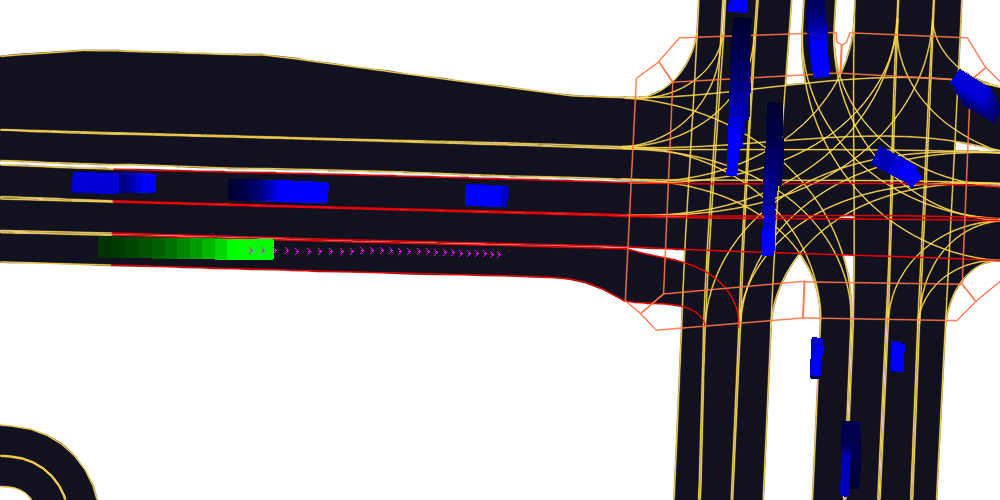
\includegraphics[width=\linewidth]{raster_l5kit.png}
    \caption{Wizualizacja rasteryzatora \texttt{SemBoxRasterizer}}
\end{figure}

\newpage

Biblioteka \texttt{l5kit} posiada klasę \texttt{SemBoxRasterizer}, która pozwala rasteryzować dane bez konieczności własnej implementacji rasteryzatora. Klasa \texttt{SemBoxRasterizer} posiada rozwiązania, które mogą znacząco wpływać na skuteczność predykcji np. kolorowanie historycznych pozycji ciemniejszymi kolorami (im wcześniejsza tym ciemniejsza), zaznaczanie pozycji przejść dla pieszych, zaznaczanie krawędzi prawej oraz lewej pasa w każdym miejscu (nawet na skrzyżowaniach, co jest czasem trudne w interpretacji). Następny rasteryzator posiada rozwiązania, które mają za zadanie uprościć rasteryzowany obraz w nadzieji na to, że modele uczące się na tych obrazach będą uczyć się szybciej i dokładniej.

\section{Rasteryzator \texttt{CenterLines}}

\begin{figure}[htbp]
    \centering
    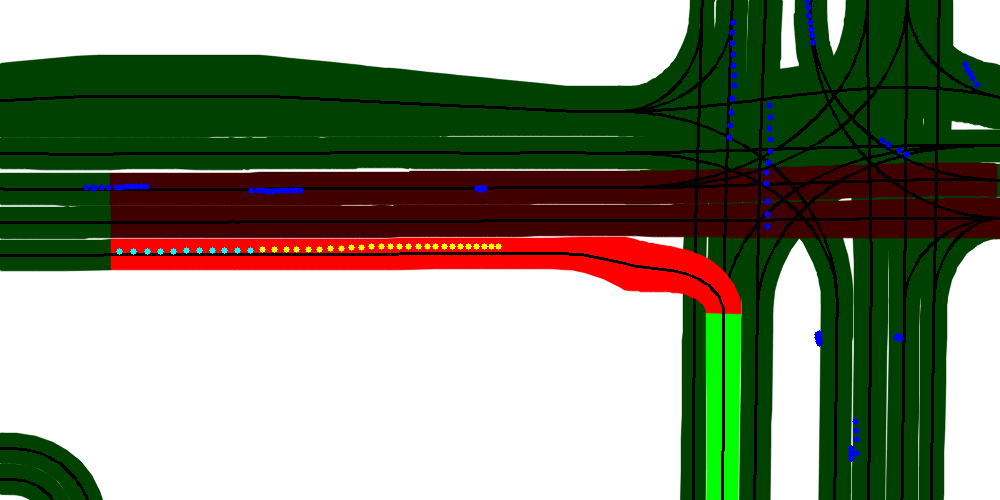
\includegraphics[width=\linewidth]{raster_custom.png}
    \caption{Wizualizacja rasteryzatora \texttt{CenterLines}}
\end{figure}

Rasteryzator CenterLines został zaprojektowany mając na uwadze maksymalne uproszczenie rasteryzowanej sceny, co potencjalnie mogłoby wpłynąć pozytywnie na skuteczność predykcji. Rzeczy które zostały zrobione inaczej w tym rasteryzatorze:

\begin{itemize}
    \item Agenci zaznaczeni są jako kropki o stałym rozmiarze, bez zaznaczania wcześniejszych pozycji ciemniejszym kolorem (uproszczenie, które miało na celu ułatwienie procesu trenowania)
    \item Wejściowe pozycje agenta \texttt{EGO} są zaznaczone kolorem seledynowym, pozycje wyjściowe są zaznaczone na żółto. Ważne jest, że pozycje wyjściowe są tylko poglądowe (nie występują ani w zbiorze treningowym, ani w zbiorze testowym). Tak więc nie mają w żadnym stopniu wpływu na proces trenowania i przewidywania.
    \item Nie występują krawędzie prawa i lewa zaznaczone odpowiednimi kolorami, te krawędzie zostały zastąpione pasem pokolorowanym na zielono, jeśli światła wskazują, że można nim jechać, lub czerwonym w przeciwnym wypadku. Krawędzie prawa i lewa zostały połączone w krawędź środkową pasa. Krawędź ta wyznacza możliwe kierunki w jakich może się poruszać agent.
    \item Pasy, które są osiągalne dla agenta \texttt{EGO} bez zmiany pasa z aktualnej pozycji, zostały wyróżnione jaśniejszymi kolorami, te do których agent \texttt{EGO} nie może dotrzeć bez zmiany pasa zostały zaciemnione.
\end{itemize}

\newpage

\section{Algorytm wyznaczania środka pasa \texttt{AWSP}}

Do wyznaczenia środka pasa na podstawie prawej i lewej krawędzi został zaimplementowany algorytm interpolujący \texttt{AWSP}. Algorytm został opisany w pseudokodzie, a samo działanie algorytmu zostało przedstawione na wykresach dotyczących przykładowego kawałka pasa ruchu.

\subsection{Opis danych wejściowych i wynikowych}

\vspace{0em}
\begin{minted}{python}
lane_in = {
    'xyz_left': np.array([[x_0, y_0, z_0], ... [x_n, y_n, z_n]]),   # lewa krawędź
    'xyz_right': np.array([[x_0, y_0, z_0], ... [x_m, y_m, z_m]]),  # prawa krawędź
    'lights': lights_color                                          # sygnalizacja pasa
}

lane_out = {
    'xy_left': np.array([[x_0, y_0], ... [x_n, y_n]]),              # lewa krawędź
    'xy_right': np.array([[x_0, y_0], ... [x_m, y_m]]),             # prawa krawędź
    'xy_center': np.array([[x_0, y_0], ... [x_k, y_k]]),            # środkowa krawędź
    'lights': lights_color                                          # sygnalizacja pasa
}
\end{minted}

\subsection{Pseudokod algorytmu \texttt{AWSP}}

\begin{pseudokod}[H]
    \SetAlgoLined
    \DontPrintSemicolon
    \textbf{Dane wejściowe:} $lane\_in$\;
    \textbf{Dane wynikowe:} $lane\_out \leftarrow \{\;\}$\;
    
    \BlankLine
    \For{$side$ $\in$ \text{\upshape \lbrack}$left$, $right$\text{\upshape \rbrack}}{
        $d \leftarrow pairwise\_L2\_norm(lane\_in['xyz\_side'])$\Comment*[r]{Odległości sąsiednich węzłów interpolacji krawędzi}
        $d \leftarrow cumulative\_sum(d)$\Comment*[r]{Odległości od pierwszego węzła interpolacji}
        $side\_l \leftarrow d[-1]$\Comment*[r]{Długość krawędzi (odległość od pierwszego węzła do ostatniego)}
        $t \leftarrow d / max(d)$\Comment*[r]{Wektor rosnących wartości parametru $t \in [0, 1]$}
        $side\_fx \leftarrow interpolating\_f(t,lane\_in['xyz\_side']['x'])$\Comment*[r]{Funkcja $x(t)$ danej krawędzi}
        $side\_fy \leftarrow interpolating\_f(t,lane\_in['xyz\_side']['y'])$\Comment*[r]{Funkcja $y(t)$ danej krawędzi}
    }
    
    \BlankLine
    $n \leftarrow \lceil max(left\_l, right\_l) / 0.5 \rceil$\Comment*[r]{Optymalna ilość węzłów interpolacji}
    $t \leftarrow \lbrack 0, 1, ... , n-1, n \rbrack/n$\Comment*[r]{Wartości węzłów interpolacji}
    
    \BlankLine
    \For{$side$ $\in$ \text{\upshape \lbrack}$left$, $right$\text{\upshape \rbrack}}{
        $side\_xy \leftarrow [side\_fx(t), side\_fy(t)]$\Comment*[r]{Interpolowane wartości współrzędnych xy danej krawędzi}
    }
    
    \BlankLine
    $lane\_out['xy\_center'] \leftarrow (left\_xy + right\_xy)/2$\Comment*[r]{Środek pasa to ciąg punktów środkowych}
    $lane\_out['xy\_right'] \leftarrow lane\_in['xyz\_right']['xy']$\;
    $lane\_out['xy\_left'] \leftarrow lane\_in['xyz\_left']['xy']$\;
    $lane\_out['lights'] \leftarrow lane\_in['lights']$\;
    
    \BlankLine
    \textbf{return} $lane\_out$

    \caption{Algorytm AWSP}
\end{pseudokod}

\newpage

\subsection{Wizualizacja algorytmu \texttt{AWSP}}

\begin{figure}[H]
    \centering
    \subfloat[Współrzędna x środka pasa w zależności od parametru t]{\includesvg[width=0.5\textwidth]{center_lane_vis_1.svg}}
    \subfloat[Współrzędna y środka pasa w zależności od parametru t]{\includesvg[width=0.5\textwidth]{center_lane_vis_2.svg}}
\end{figure}

\begin{figure}[H]
    \centering
    \subfloat[Węzły interpolacji rozważanego kawałka pasa jezdni]{\includesvg[width=0.5\textwidth]{center_lane_vis_0.svg}}
    \subfloat[Uzyskany środek pasa ruchu]{\includesvg[width=0.5\textwidth]{center_lane_vis_3.svg}}
\end{figure}

\newpage

\subsection{Implementacja algorytmu \texttt{AWSP}}

\vspace*{0.5cm}

\begin{minted}{python}
import numpy as np
from scipy.interpolate import interp1d

def algorithm_awsp(lane_in):
    lights = lane_in['lights'] # kolor świateł
    lane_l = lane_in['xyz_left'][:, :2] # współrzędne xyz węzłów lewej krawędzi pasa
    lane_r = lane_in['xyz_right'][:, :2] # współrzędne xyz węzłów prawej krawędzi pasa
    # współrzędne węzłów lane_l oraz lane_r są przedstawione na rysunku (c)
    
    # odległości pomiędzy kolejnymi węzłami
    lane_l_dist = np.linalg.norm(lane_l[1:] - lane_l[:-1], axis=1)
    lane_l_dist = np.cumsum(lane_l_dist) # odległości po krawędzi do pierwszego węzła
    l_total_dist = lane_l_dist[-1] # długość krawędzi
    lane_l_dist = np.concatenate([[0], lane_l_dist]) # uwzględnienie pierwszego węzła
    lane_l_t = lane_l_dist / lane_l_dist[-1] # wyznaczenie parametru t dla każdego węzła

    lane_r_dist = np.linalg.norm(lane_r[1:] - lane_r[:-1], axis=1)
    lane_r_dist = np.cumsum(lane_r_dist)
    r_total_dist = lane_r_dist[-1]
    lane_r_dist = np.concatenate([[0], lane_r_dist])
    lane_r_t = lane_r_dist / lane_r_dist[-1]

    # inicjalizacja funkcji interpolujących liniowo współrzędne węzłów w zależności od t
    l_x_interp = interp1d(lane_l_t, lane_l[:, 0]) 
    l_y_interp = interp1d(lane_l_t, lane_l[:, 1])
    r_x_interp = interp1d(lane_r_t, lane_r[:, 0])
    r_y_interp = interp1d(lane_r_t, lane_r[:, 1])

    # liczba węzłów krawędzi środkowej (minimum 1 węzeł na 0.5m, w sumie minimum 3 węzły)
    steps = max(int(np.ceil(max(l_total_dist, r_total_dist) / 0.5)), 3)
    # wektor wartości parametru t, używany do wyliczenia węzłów krawędzi środkowej
    steps_vec = np.arange(steps)/(steps - 1)

    # obliczanie współrzędnych x krawędzi środkowej, przedstawione na rysunku (a)
    mid_points_x = (l_x_interp(steps_vec) + r_x_interp(steps_vec)) / 2.0
    
    # obliczanie współrzędnych y krawędzi środkowej, przedstawione na rysunku (b)
    mid_points_y = (l_y_interp(steps_vec) + r_y_interp(steps_vec)) / 2.0
    
    # współrzędne xy krawędzi środkowej, przedstawione na rysunku (d)
    mid_points = np.stack([mid_points_x, mid_points_y], axis=0).T

    lane_out = {
        'xy_left': lane_l,
        'xy_right': lane_r,
        'xy_center': mid_points,
        'lights': lights
    }

    return lane_out
\end{minted}


\newpage

\section{Algorytm wyznaczania osiągalnych pasów \texttt{AWOP}}

W rasteryzatorze \texttt{CenterLines} pasy, które są osiągalne przez agenta \texttt{EGO} bez zmiany pasa są zaznaczone jaśniejszym kolorem. Aby takie kolorowanie było możliwe trzeba najpierw wyznaczyć te pasy. Dla każdej sceny możliwe jest uzyskanie listy wszystkich pasów zawartych przynajmniej częściowo na tej scenie. Dla każdego elementu z tej listy (pas drogowy), wyznaczany jest następnie środek pasa za pomocą algorytmu \texttt{AWSP}. Elementy te można następnie wykorzystać do zbudowania reprezentacji grafowej mapy za pomocą algorytmu \texttt{AWOP}. Kąt odchylenia najbliższego pasa będzie przydatny w dalszych etapach podczas normalizacji sceny.

\subsection{Opis danych wejściowych i wynikowych}

\vspace{0em}
\begin{minted}{python}
lanes_in = [                                                  # lista pasów ruchu
    {
        'xy_left': np.array([[x_0, y_0], ... [x_n, y_n]]),    # lewa krawędź
        'xy_right': np.array([[x_0, y_0], ... [x_m, y_m]]),   # prawa krawędź
        'xy_center': np.array([[x_0, y_0], ... [x_k, y_k]]),  # środkowa krawędź
        'lights': lights_color                                # sygnalizacja na pasie
    },
    ...
]

agent_ego_in = np.array([                                     # wejściowe współrzędne
    [x_0, y_0],                                               # agenta EGO
    ...                                                       # lista 11 punktów xy
    [x_10, y_10]
])

lanes_out = [                                                 # lista pasów ruchu
    {
        'xy_left': np.array([[x_0, y_0], ... [x_n, y_n]]),    # lewa krawędź
        'xy_right': np.array([[x_0, y_0], ... [x_m, y_m]]),   # prawa krawędź
        'xy_center': np.array([[x_0, y_0], ... [x_k, y_k]]),  # środkowa krawędź
        'lights': lights_color,                               # sygnalizacja na pasie
        'reachable': lane_reachability_status                 # True/False status
    },                                                        # osiągalności pasa
    ...
]

yaw_out = agent_ego_closest_lane_yaw                          # kąt odchylenia pasa
                                                              # najbliższego agentowi EGO
\end{minted}

\subsection{Pseudokod algorytmu \texttt{AWOP}}

\begin{pseudokod}[H]
    \SetAlgoLined
    \DontPrintSemicolon
    \textbf{Dane wejściowe:} $lanes\_in, agent\_ego\_in$\;
    \textbf{Dane wynikowe:} $lanes\_out, yaw\_out$\;
    
    \BlankLine
    $lanes\_out \leftarrow get\_graph\_representation(lanes\_in)$\Comment*[r]{Przypisanie każdemu pasowi 2 wierzchołków grafu}
    $idx \leftarrow get\_ego\_closest\_lane(lanes\_out, agent\_ego\_in)$\Comment*[r]{Pas najbliższy pozycjom wejściowym agenta EGO}
    $lanes\_out \leftarrow get\_reachability(lanes\_out, idx)$\Comment*[r]{Dodanie do pasów informacji o osiągalności}
    $yaw\_out \leftarrow get\_closest\_lane\_yaw(lanes\_out, agent\_ego\_in, idx)$\Comment*[r]{Kąt odchylenia najbliższego pasa}
    
    \BlankLine
    \textbf{return} $lanes\_out, yaw\_out$

    \caption{Algorytm AWOP}
\end{pseudokod}

\newpage

\subsection{Funkcje pomocnicze algorytmu \texttt{AWOP}}

\subsubsection{Pseudokod funkcji \texttt{get\_graph\_representation}}

\begin{pseudokod}[H]
    \SetAlgoLined
    \DontPrintSemicolon
    \textbf{Dane wejściowe:} $lanes\_list$\;
    \textbf{Dane wynikowe:} $lanes\_list$\;
    
    \BlankLine
    $nodes \leftarrow \lbrack\;\rbrack$\;
    $unique\_nodes \leftarrow \lbrack\;\rbrack$\;
    
    \BlankLine
    \For{$lane$ $\in$ $lanes\_list$}{
        $nodes.append(lane['xy\_center'].first)$\Comment*[r]{Pierwszy węzeł interpolacji jako wierzchołek grafu}
        $nodes.append(lane['xy\_center'].last)$\Comment*[r]{Ostatni węzeł interpolacji jako wierzchołek grafu}
    }
    
    \BlankLine
    \For{$node$ $\in$ $nodes$}{
        \uIf{$len(nodes) == 0\:\textbf{\upshape or}\:min\_distance(unique\_nodes, node) < \epsilon$}{
            $unique\_nodes.append(node)$\Comment*[r]{Jest dodany jeśli nie ma podobnego wierzchołka w liście}
        }
    }
    
    \BlankLine
    \For{$lane$ $\in$ $lanes\_list$}{
        $lane['node\_0'] \leftarrow closest\_idx(unique\_nodes, lane['xy\_center'].first)$\Comment*[r]{Indeks najbliższego wierzchołka}
        $lane['node\_1'] \leftarrow closest\_idx(unique\_nodes, lane['xy\_center'].last)$\Comment*[r]{Indeks najbliższego wierzchołka}
    }
    
    \BlankLine
    \textbf{return} $lanes\_list$

    \caption{Funkcja get\_graph\_representation}
\end{pseudokod}

\subsubsection{Implementacja funkcji \texttt{get\_graph\_representation}}

\begin{minted}{python}
def graph_representation(lanes_list):
    nodes = []
    unique_nodes = []

    for lane in lanes_list:
        nodes.append(lane['xy_center'][0])
        nodes.append(lane['xy_center'][-1])

    for node in nodes:
        if len(unique_nodes) == 0:
            unique_nodes.append(node)
        elif np.min(np.linalg.norm(np.array(unique_nodes) - node, axis=1)) > 0.1:
            unique_nodes.append(node)

    for lane in lanes_list:
        lane['node_0'] = np.argmin(np.linalg.norm(
            np.array(unique_nodes) - lane['xy_center'][0], axis=1
        ))
        lane['node_1'] = np.argmin(np.linalg.norm(
            np.array(unique_nodes) - lane['xy_center'][-1], axis=1
        ))

    return lanes_list
\end{minted}

\newpage

\subsubsection{Pseudokod funkcji \texttt{get\_ego\_closest\_lane}}

\begin{pseudokod}[H]
    \SetAlgoLined
    \DontPrintSemicolon
    \textbf{Dane wejściowe:} $lanes\_list, agent\_ego$\;
    \textbf{Dane wynikowe:} $closest\_lane\_idx$\;
    
    \BlankLine
    $d \leftarrow matrix(agent\_ego.size, lanes\_list.size)$\Comment*[r]{Odległości pozycji agenta EGO do węzłów środka pasa}

    \BlankLine
    \For{$i = 0;\ i < agent\_ego.size;\ i = i + 1$}{
        \For{$j = 0;\ j < lanes\_list.size;\ j = j + 1$}{
            $l \leftarrow lanes\_list[j]['xy\_center']$\Comment*[r]{Współrzędne środka jednego z pasów sceny}
            $d[i][j] \leftarrow min\_distance(l, agent\_ego[i])$\Comment*[r]{Odległość jednej pozycji agenta EGO do środka pasa}
        }
    }
    
    \BlankLine
    $idxs \leftarrow agent\_pos\_closest\_lanes(d)$\Comment*[r]{Pasy, które były najbliższe pozycjom agenta EGO}
    $closest\_lane\_idx \leftarrow most\_common\_number(idxs)$\Comment*[r]{Pas, który był najbliższy najczęściej}
    
    \BlankLine
    \textbf{return} $closest\_lane\_idx$

    \caption{Funkcja get\_ego\_closest\_lane}
\end{pseudokod}

\subsubsection{Wizualizacja funkcji \texttt{get\_ego\_closest\_lane}}

\vspace{-1cm}
\begin{figure}[H]
    \centering
    \subfloat[Widok \texttt{BEV} na rozważaną scenę]{\includesvg[width=0.5\textwidth]{most_common_lane.svg}}
    \subfloat[Najbliższy pas drogi dla agenta EGO]{\includesvg[width=0.5\textwidth]{most_common_lane_zoom.svg}}
\end{figure}

\subsubsection{Implementacja funkcji \texttt{get\_ego\_closest\_lane}}

\begin{minted}{python}
def get_ego_closest_lane(lanes_list, agent_ego):
    distances = np.zeros((agent_ego.shape[0], len(lanes_list)))

    for i in range(agent_ego.shape[0]):
        for j, lane in enumerate(lanes_list):
            distances[i, j] = np.min(np.linalg.norm(
                lane['xy_center'] - agent_ego[i],
                axis=1
            ))

    closest_lanes_idxs = np.argmin(distances, axis=1).tolist()
    closest_lane_idx = max(set(closest_lanes_idxs), key=closest_lanes_idxs.count)

    return closest_lane_idx
\end{minted}

\subsubsection{Pseudokod funkcji \texttt{get\_reachability}}

\begin{pseudokod}[H]
    \SetKwProg{Fn}{function}{:}{}
    \SetAlgoLined
    \DontPrintSemicolon
    \textbf{Dane wejściowe:} $lanes\_list, closest\_lane\_idx$\;
    \textbf{Dane wynikowe:} $lanes\_list$\;
    
    \BlankLine
    \For{$lane$ $\in$ $lanes\_list$}{
        $lane['dir\_adjacent\_lanes'] \leftarrow get\_adjacent\_lanes(lanes\_list)$\Comment*[r]{Pasy kontynuujące dany pas}
        $lane['reachable'] \leftarrow \text{\upshape false}$\Comment*[r]{Na początku żaden pas nie jest osiągalny}
    }
    
    \BlankLine
    \Fn{$depth\_first\_search(lane)$}{
        \uIf{$lane['reachable'] == \text{\upshape false}$}{
            $lane['reachable'] \leftarrow \text{\upshape true}$\Comment*[r]{Pas został odwiedzony, więc jest osiągalny}
            
            \BlankLine
            \For{$lane\_adjacent$ $\in$ $lane['dir\_adjacent\_lanes']$}{
                $depth\_first\_search(lane\_adjacent)$\Comment*[r]{Odwiedzanie pasów kontynuujących pas}
            }
        }
    }
    
    \BlankLine
    $depth\_first\_search(lanes\_list[closest\_lane\_idx])$\Comment*[r]{Inicjalizacja pasem najbliższym agentowi EGO}
    
    \BlankLine
    \textbf{return} $lanes\_list$
    
    \caption{Funkcja get\_reachability}
\end{pseudokod}

\subsubsection{Wizualizacja funkcji \texttt{get\_reachability}}

\begin{figure}[H]
    \centering
    \includesvg[width=0.48\textwidth]{reachability_1.svg}
    \includesvg[width=0.48\textwidth]{reachability_3.svg}
    \\[-2ex]
    \includesvg[width=0.48\textwidth]{reachability_5.svg}
    \includesvg[width=0.48\textwidth]{reachability_7.svg}
    \caption{Kolejne iteracje algorytmu \texttt{DFS} w funkcji \texttt{get\_reachability}}
\end{figure}

\newpage

\subsubsection{Implementacja funkcji \texttt{get\_reachability}}

\begin{minted}{python}
def get_reachability(lanes_list, closest_lane_idx):
    for lane in lanes_list:
        lane['dir_adjacent_lanes'] = [
            x for x in lanes_list if lane['node_1'] == x['node_0']
        ]

    def dfs(lane):
        if not lane['reachable']:
            lane['reachable'] = True

            for lane_adjacent in lane['dir_adjacent_lanes']:
                dfs(lane_adjacent)

    dfs(lanes_list[closest_lane_idx])

    return lanes_list
\end{minted}

\subsubsection{Pseudokod funkcji \texttt{get\_closest\_lane\_yaw}}

\begin{pseudokod}[H]
    \SetAlgoLined
    \DontPrintSemicolon
    \textbf{Dane wejściowe:} $lanes\_list, agent\_ego, closest\_lane\_idx$\;
    \textbf{Dane wynikowe:} $lane\_yaw$\;
    
    \BlankLine
    $interp\_nodes \leftarrow lanes\_list[closest\_lane\_idx]['xy\_center']$\Comment*[r]{Węzły interpolacji środka pasa}
    $idx \leftarrow argmin\_distance(interp\_nodes, agent\_ego[0])$\Comment*[r]{Węzeł najbliższy obecnej pozycji agenta EGO}
    
    \BlankLine
    \uIf{$next\_node\_exists(idx)$}{
        $p\_0 \leftarrow interp\_nodes[idx]$\Comment*[r]{Dwa punkty pozwalające obliczyć odchylenie}
        $p\_1 \leftarrow interp\_nodes[idx + 1]$\;
    }
    \uElseIf{$prev\_node\_exists(interp\_node\_idx)$}{
        $p\_0 \leftarrow interp\_nodes[idx - 1]$\Comment*[r]{Dwa punkty pozwalające obliczyć odchylenie}
        $p\_1 \leftarrow interp\_nodes[idx]$\;
    }
    \Else{
        $p\_0 \leftarrow agent\_ego[0]$\Comment*[r]{Jeśli nie ma pasa, odchylenie uzyskuje się z pozycji agenta EGO}
        $p\_1 \leftarrow agent\_ego[1]$\;
    }
    
    \BlankLine
    $lane\_yaw \leftarrow get\_vec\_yaw(p\_1 - p\_0)$\Comment*[r]{Obliczanie kąta odchylenia z wektora przemieszczenia}
    
    \BlankLine
    \textbf{return} $lane\_yaw$

    \caption{Funkcja get\_closest\_lane\_yaw} 
\end{pseudokod}

\newpage

\subsubsection{Wizualizacja funkcji \texttt{get\_closest\_lane\_yaw}}
\vspace{-1cm}
\begin{figure}[H]
    \centering
    \subfloat{\includesvg[width=0.5\textwidth]{lane_angle.svg}}
    \subfloat{\includesvg[width=0.5\textwidth]{lane_angle_zoom.svg}}
\end{figure}

\subsubsection{Implementacja funkcji \texttt{get\_closest\_lane\_yaw}}

\begin{minted}{python}
def get_closest_lane_yaw(lanes_list, agent_ego, closest_lane_idx):
    interp_nodes = lanes_list[closest_lane_idx]['xy_center']
    interp_node_idx = np.argmin(np.linalg.norm(
        interp_nodes - agent_ego[0],
        axis=1
    ))

    if interp_node_idx + 1 < interp_nodes.shape[0]:
        p_0 = interp_nodes[interp_node_idx]
        p_1 = interp_nodes[interp_node_idx + 1]
    elif interp_node_idx - 1 >= 0:
        p_0 = interp_nodes[interp_node_idx - 1]
        p_1 = interp_nodes[interp_node_idx]
    else:
        p_0 = agent_ego[0]
        p_1 = agent_ego[1]

    dir_vec = p_0 - p_1
    dir_vec = dir_vec[0] + dir_vec[1] * 1j
    lane_yaw = np.angle(dir_vec, deg=True)

    return lane_yaw
\end{minted}

\newpage

\section{Standaryzacja danych}

Modele predykcyjne do prawidłowego działania potrzebują danych, które posiadają jak najmocniejsze zależności. W momencie gdy dane nie są ustandaryzowane np. model jest trenowany na scenach w których agenci \texttt{EGO} są zwróceni w każdym możliwym kierunku, model musi nauczyć się nie tylko przewidywać ruch agentów \texttt{EGO}, musi również robić to dla każdej możliwej orientacji agenta. Jest to o wiele trudniejsze, niż przewidywanie ruchu ze scen, które są w odpowiedni sposób ustandaryzowane. Rasteryzatory przeprowadzają następujące standaryzacje:

\begin{itemize}
    \setlength{\itemsep}{1pt}
    \setlength{\parskip}{0pt}
    \setlength{\parsep}{0pt}
    \item Obrót sceny o kąt:
    \begin{itemize}
    \item \texttt{yaw} agenta \texttt{EGO} w przypadku rasteryzatora \texttt{SemBoxRasterizer}
    \item \texttt{closest\_lane\_yaw} w przypadku rasteryzatora \texttt{CenterLines}
    \end{itemize}
    Agent po takim przekształceniu zawsze zwrócony jest na wschód.
    \item Ustalenie środka współrzędnych jako ostatniej pozycji wejściowej agenta \texttt{EGO}
    \item Środek współrzędnych na rasteryzowanym obrazie jest ustawiony w pozycji (0.25, 0.5) względem długości i szerokości obrazu. Sprawia to, że agent \texttt{EGO} ma przód zwrócony na obszar, który ma bardzo dużą powierzchnię, pozwala to sieci neuronowej lepiej wnioskować na temat możliwych trajektorii agenta.
    \item Przekształcenie współrzędnych wejściowych i wyjściowych zgodnie z poprzednimi przekształceniami
\end{itemize}

\section{Wizualizacja przekształceń}
\vspace*{-0.65cm}

\begin{figure}[h!]
    \centering
    \subfloat[Scena bez przekształceń]{\includesvg[width=0.45\textwidth]{transformations_0.svg}}
    \subfloat[Zmiana środka współrzędnych]{\includesvg[width=0.45\textwidth]{transformations_1.svg}}
    \\[-2ex]
    \subfloat[Obrót, agent \texttt{EGO} zwrócony na wschód]{\includesvg[width=0.45\textwidth]{transformations_2.svg}}
    \subfloat[Obiekty przed agentem \texttt{EGO} bardziej widoczne]{\includesvg[width=0.45\textwidth]{transformations_3.svg}}
\end{figure}
	\cleardoublepage
	
	\chapter{Funkcja kosztu}
\thispagestyle{chapterBeginStyle}

\section{Ogólny opis}
W kontekście konstruowania modelu predykcyjnego, funkcja kosztu $L$, to funkcja, która pozwala na ocenę skuteczności predykcji modelu. W tej pracy utrzymana jest konwencja minimalizowania funkcji kosztu, to znaczy, że poszukiwany jest model posiadający najmniejszą średnią wartość funkcji kosztu na ustalonym zbiorze testowym. Zadaniem funkcji kosztu jest przedstawienie skuteczności predykcji za pomocą jednej liczby w taki sposób, że proces minimalizowania wartości funkcji kosztu będzie w pewnym sensie polepszał jakość predykcji (usprawniał model). Podstawowym problemem podczas konstruowania modelu jest wybór funkcji kosztu. W tej pracy funkcją kosztu jest zaproponowana przez firmę \texttt{Lyft} funkcja $L$ opisana poniżej.

\section{Równanie funkcji kosztu}

\noindent
Załóżmy, że pozycje wyjściowe są równe:

\begin{equation}
V_{t} = [(x_{0},y_{0}), (x_{1},y_{1}), ... , (x_{49},y_{49})]
\end{equation}

\noindent
Model przewiduje trzy trajektorie i prawdopodobieństwa ($k \in \{0, 1, 2\}$):

\begin{equation}
\hat{V}_{t}^{k} = [(\hat{x}_{0}^{k},\hat{y}_{0}^{k}), (\hat{x}_{1}^{k},\hat{y}_{1}^{k}), ... , (\hat{x}_{49}^{k},\hat{y}_{49}^{k})]
\end{equation}

\begin{equation}
\hat{P}_{t}^{k} = P(\text{\upshape trajektoria}\:\hat{V}_{t}^{k}\:\text{\upshape zostanie zrealizowana})
\end{equation}

\noindent
Załóżmy, że pozycje zawarte w $V_{t}$ oraz $\hat{V}_{t}^{k}$ dotyczą chwil:

\begin{equation}
[t+0.1, t+0.2, ... , t+5.0]
\end{equation}

\noindent
Załóżmy, że pozycje wyjściowe są modelowane przez mieszaninę niezależnych wielowymiarowych rozkładów normalnych. Przy takich założeniach funkcja wiarygodności (ang. likelihood) ma postać:

\begin{equation}
p(V_{t}|\hat{P}_{t}^{0,1,2}, \hat{V}_{t}^{0,1,2}) = p(x_{0,...,49},
y_{0,...,49}|\hat{P}_{t}^{0,1,2}, \hat{V}_{t}^{0,1,2}) =
\end{equation}

\begin{equation}
= \sum_{k}\hat{P}_{t}^{k}\cdot\mathcal{N}(x_{0,...,49}|\hat{x}_{0,...,49}^{k}, \Sigma=1)\cdot\mathcal{N}(y_{0,...,49}|\hat{y}_{0,...,49}^{k}, \Sigma=1) =
\end{equation}

\begin{equation}
= \sum_{k}\hat{P}_{t}^{k}\cdot\prod_{j=0}^{j=49}\mathcal{N}(x_{j}|\mu=\hat{x}_{j}^{k}, \sigma=1)\cdot\mathcal{N}(y_{j}|\mu=\hat{y}_{j}^{k}, \sigma=1)
\end{equation}

\noindent
Tak otrzymaną funkcję wiarygodności (ang. likelihood) możemy następnie przekształcić do funkcji kosztu \texttt{NLL} (ang. negative log-likelihood):

\begin{equation}
L = -ln(p(V_{t}|\hat{P}_{t}^{0,1,2}, \hat{V}_{t}^{0,1,2})) =
\end{equation}

\begin{equation}
= -ln(\sum_{k}\hat{P}_{t}^{k}\cdot e^{-\frac{1}{2}\sum_{j=0}^{j=49}(x_{j}-\hat{x}_{j}^{k})^{2}+(y_{j}-\hat{y}_{j}^{k})^{2}}) =
\end{equation}

\newpage

\section{Wizualizacja funkcji kosztu}

\begin{figure}[H]
    \centering
    \subfloat[Wyjściowe pozycje agenta EGO]{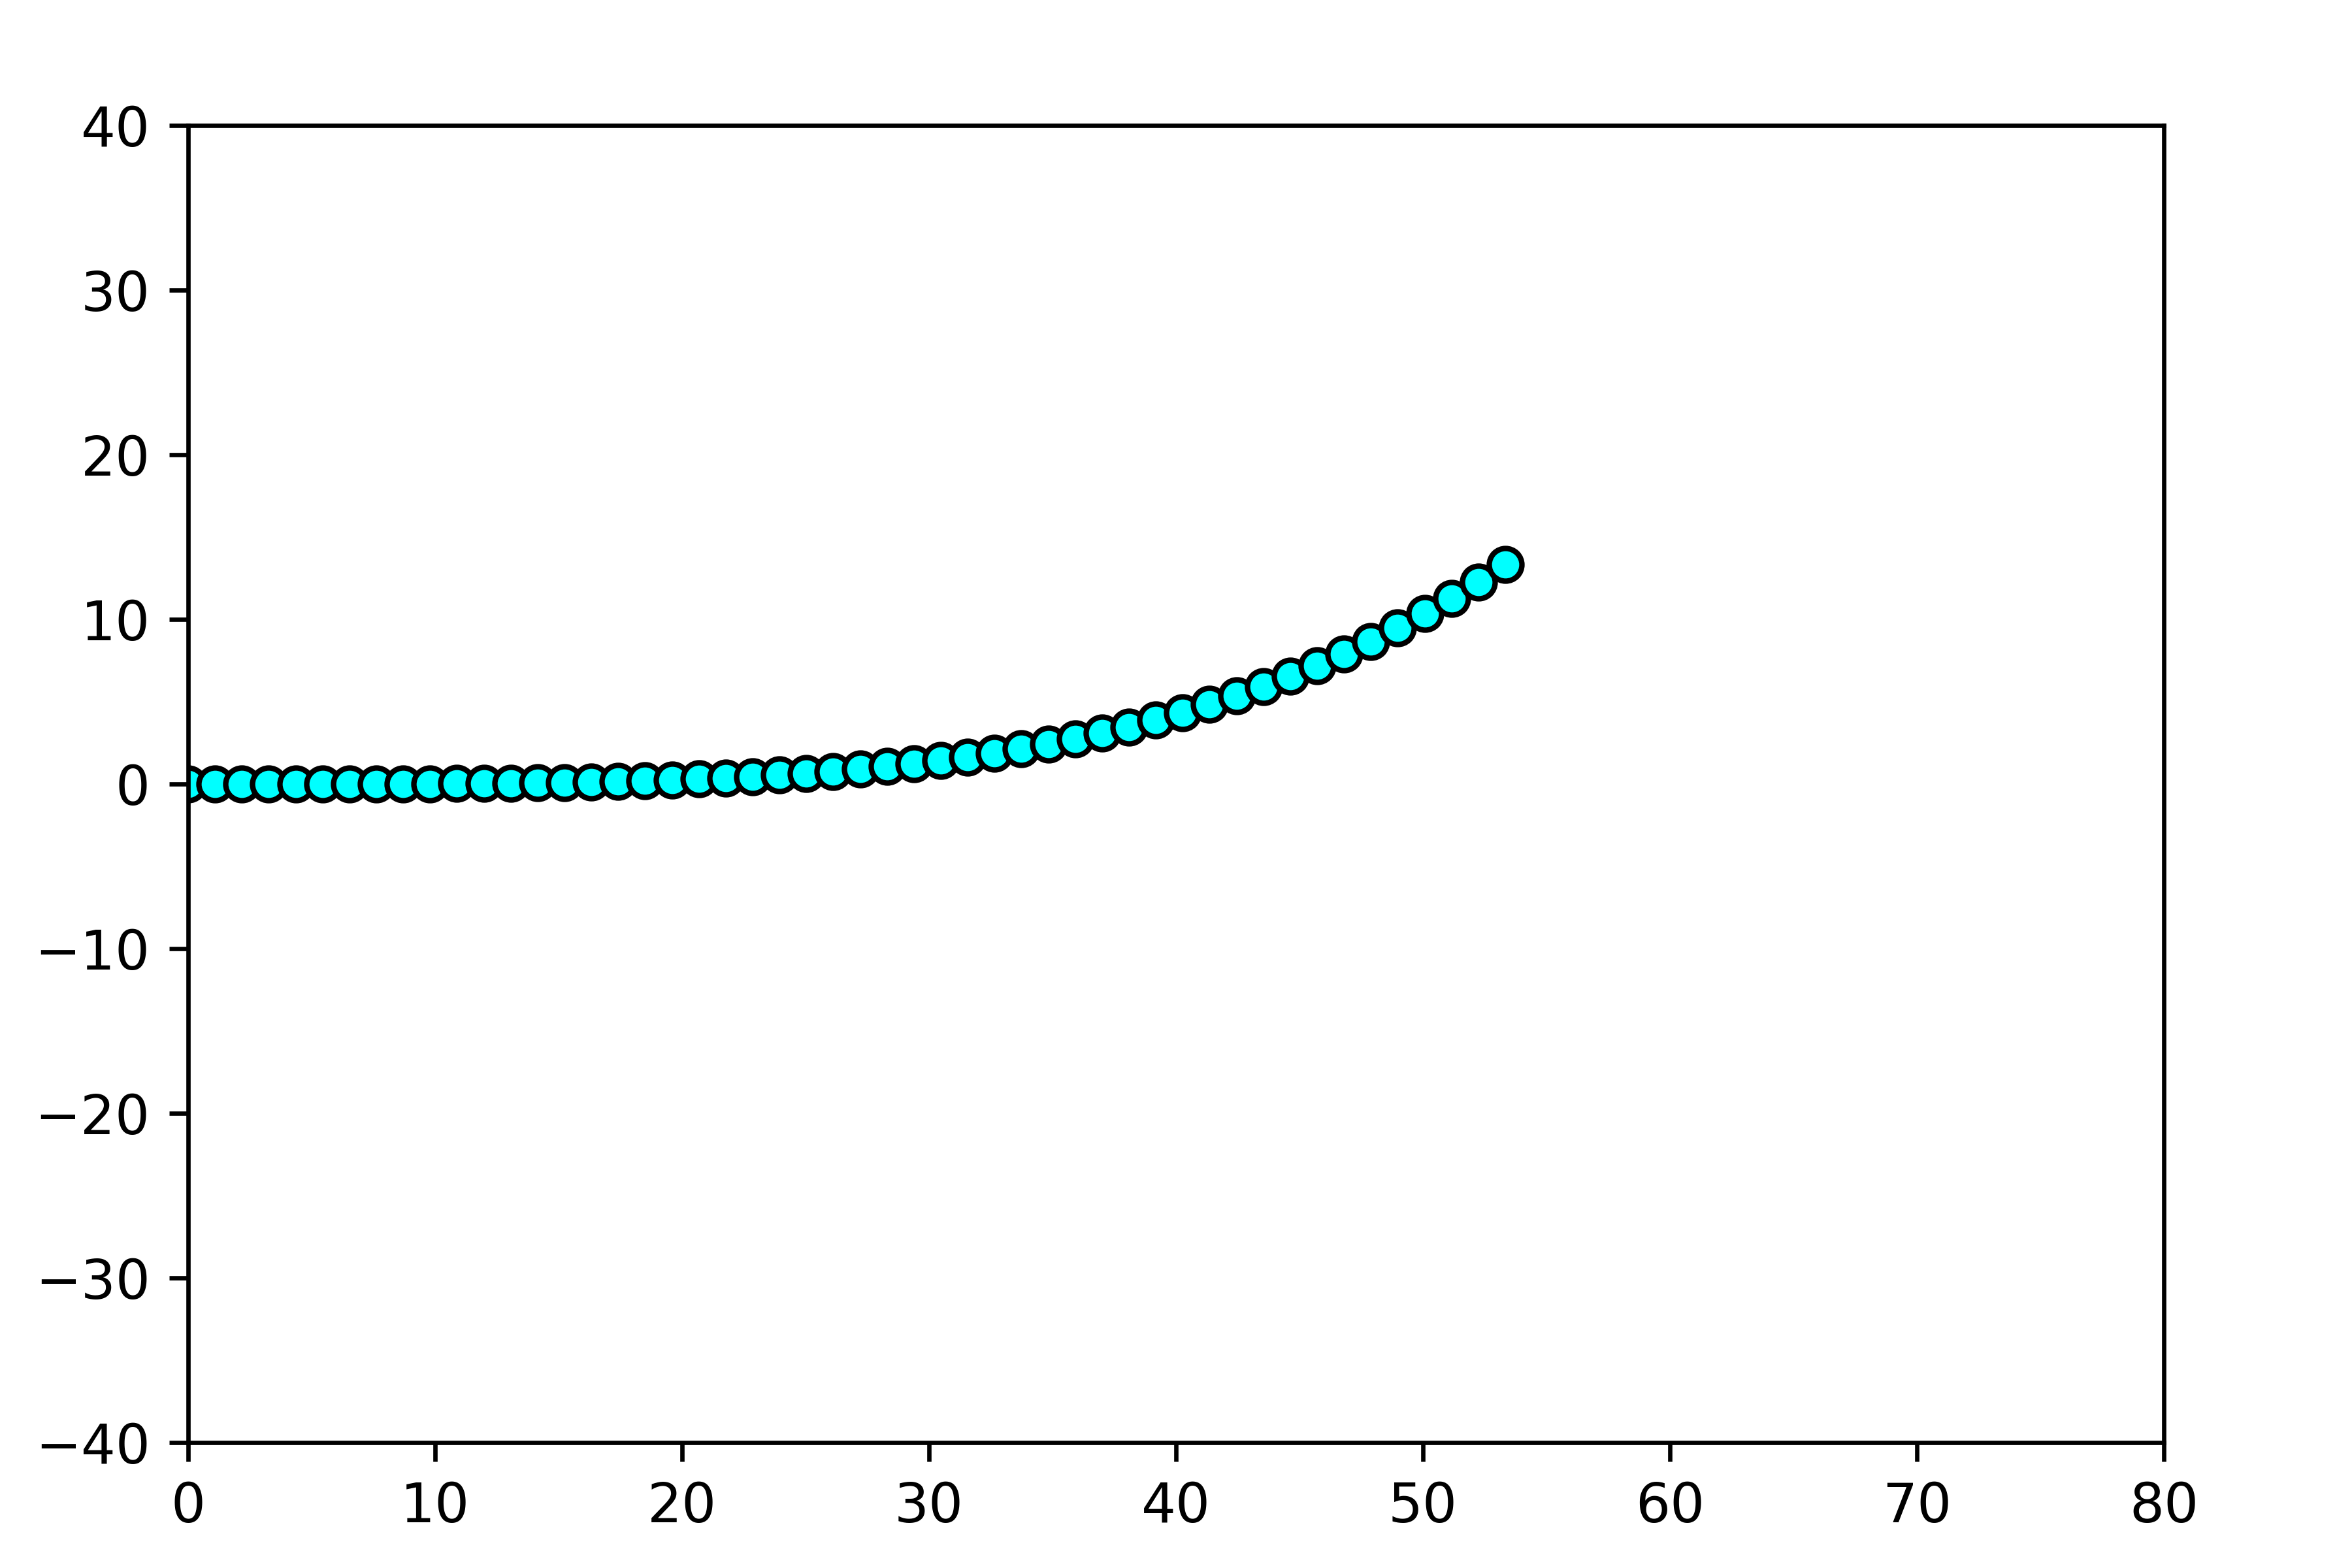
\includegraphics[width=0.5\textwidth]{loss0.png}}
    \subfloat[Trajektorie naśladujące predykcje modelu]{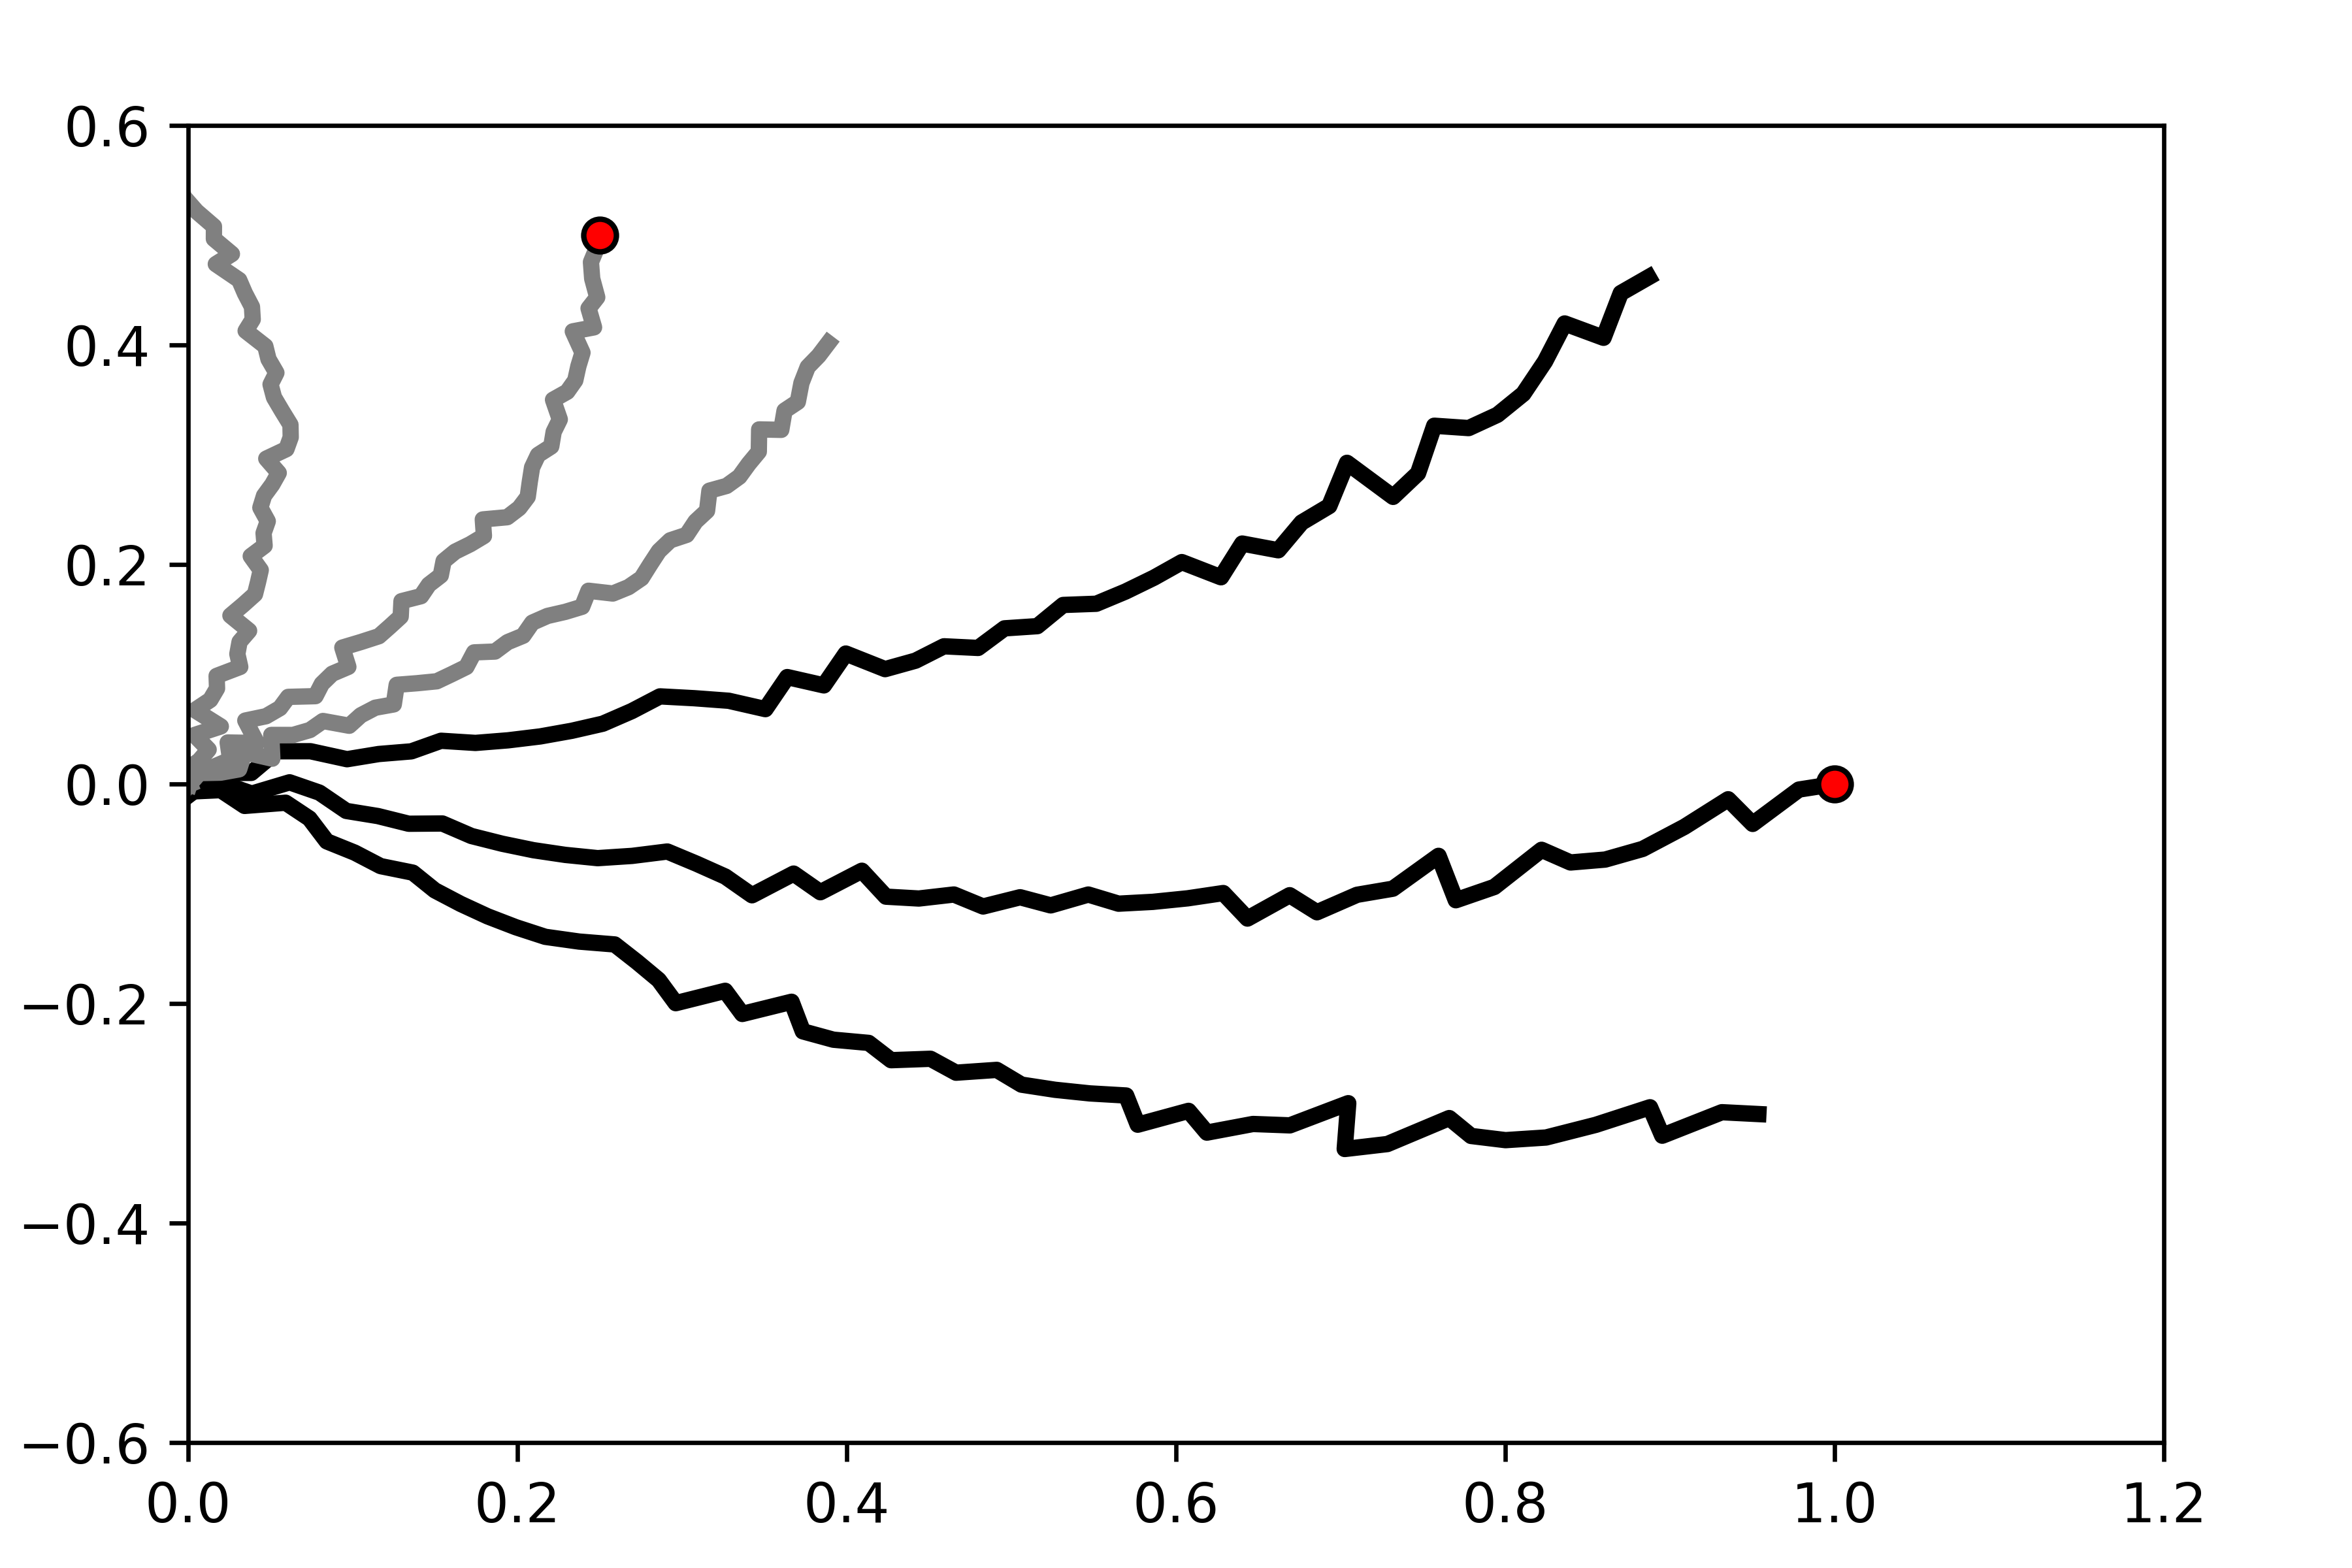
\includegraphics[width=0.5\textwidth]{loss1.png}}
\end{figure}

\begin{figure}[H]
    \centering
    \subfloat[Wartości funkcji kosztu]{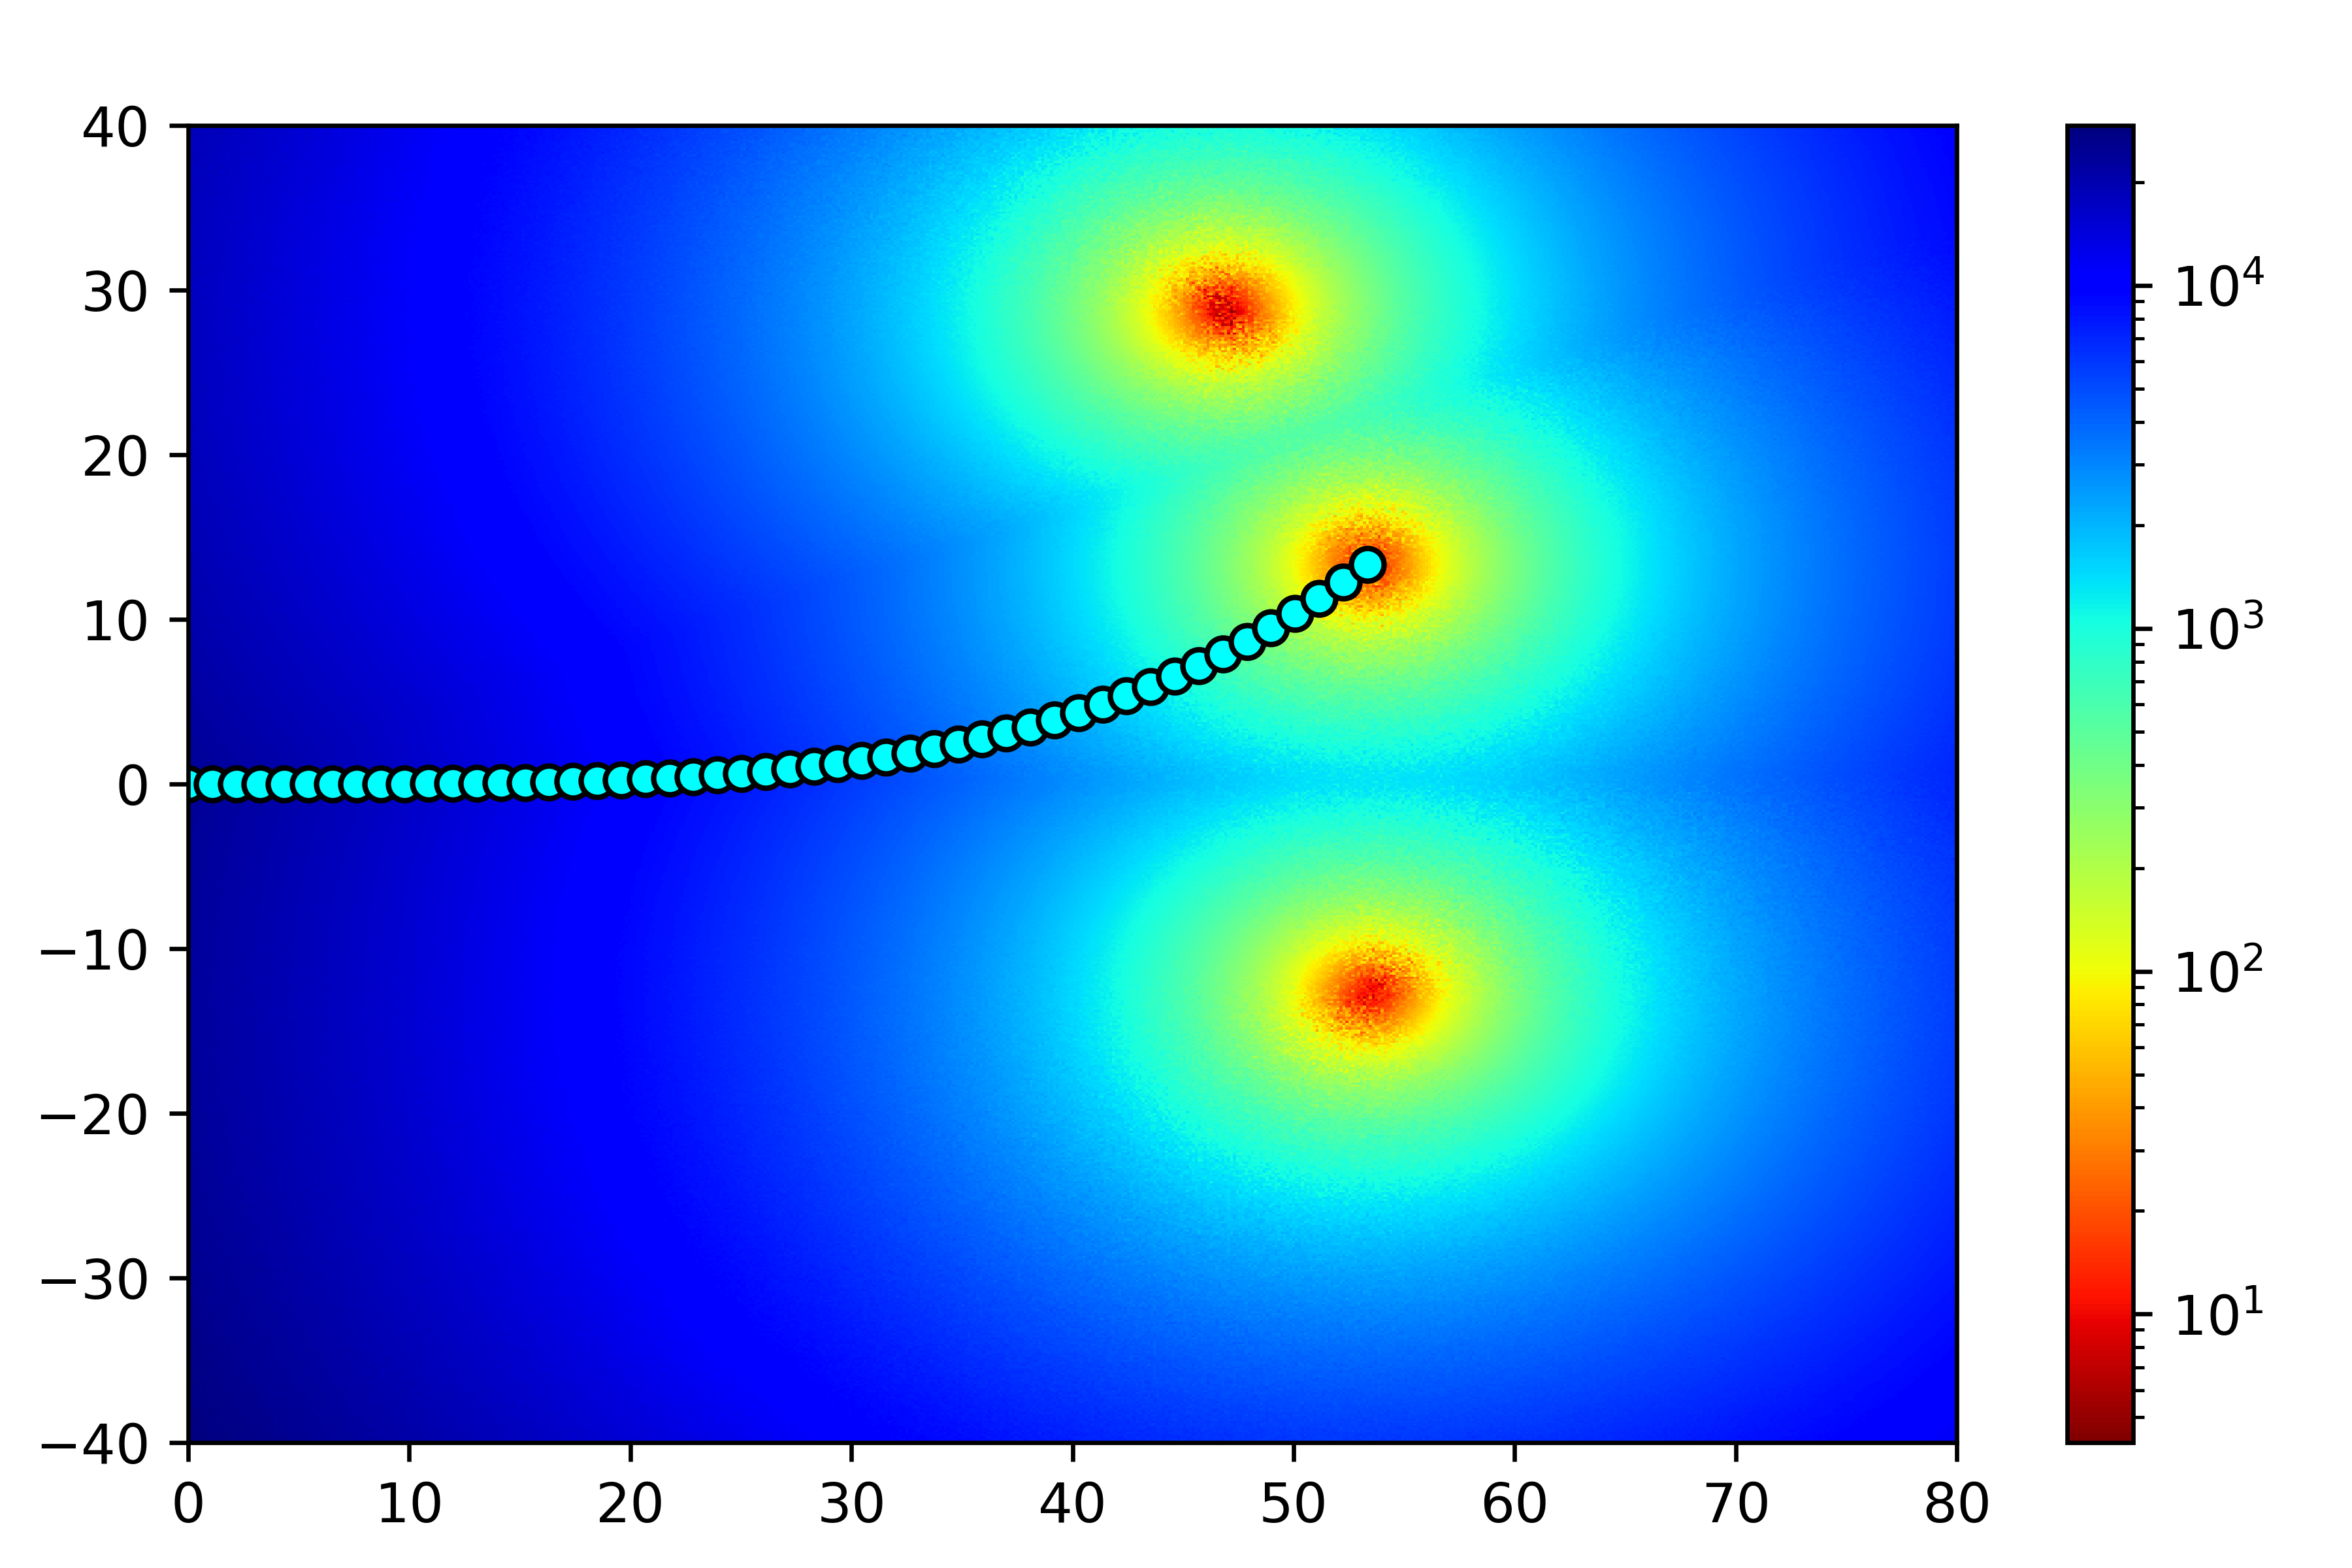
\includegraphics[width=0.5\textwidth]{loss2.png}}
    \subfloat[Pierwsze minimum lokalne]{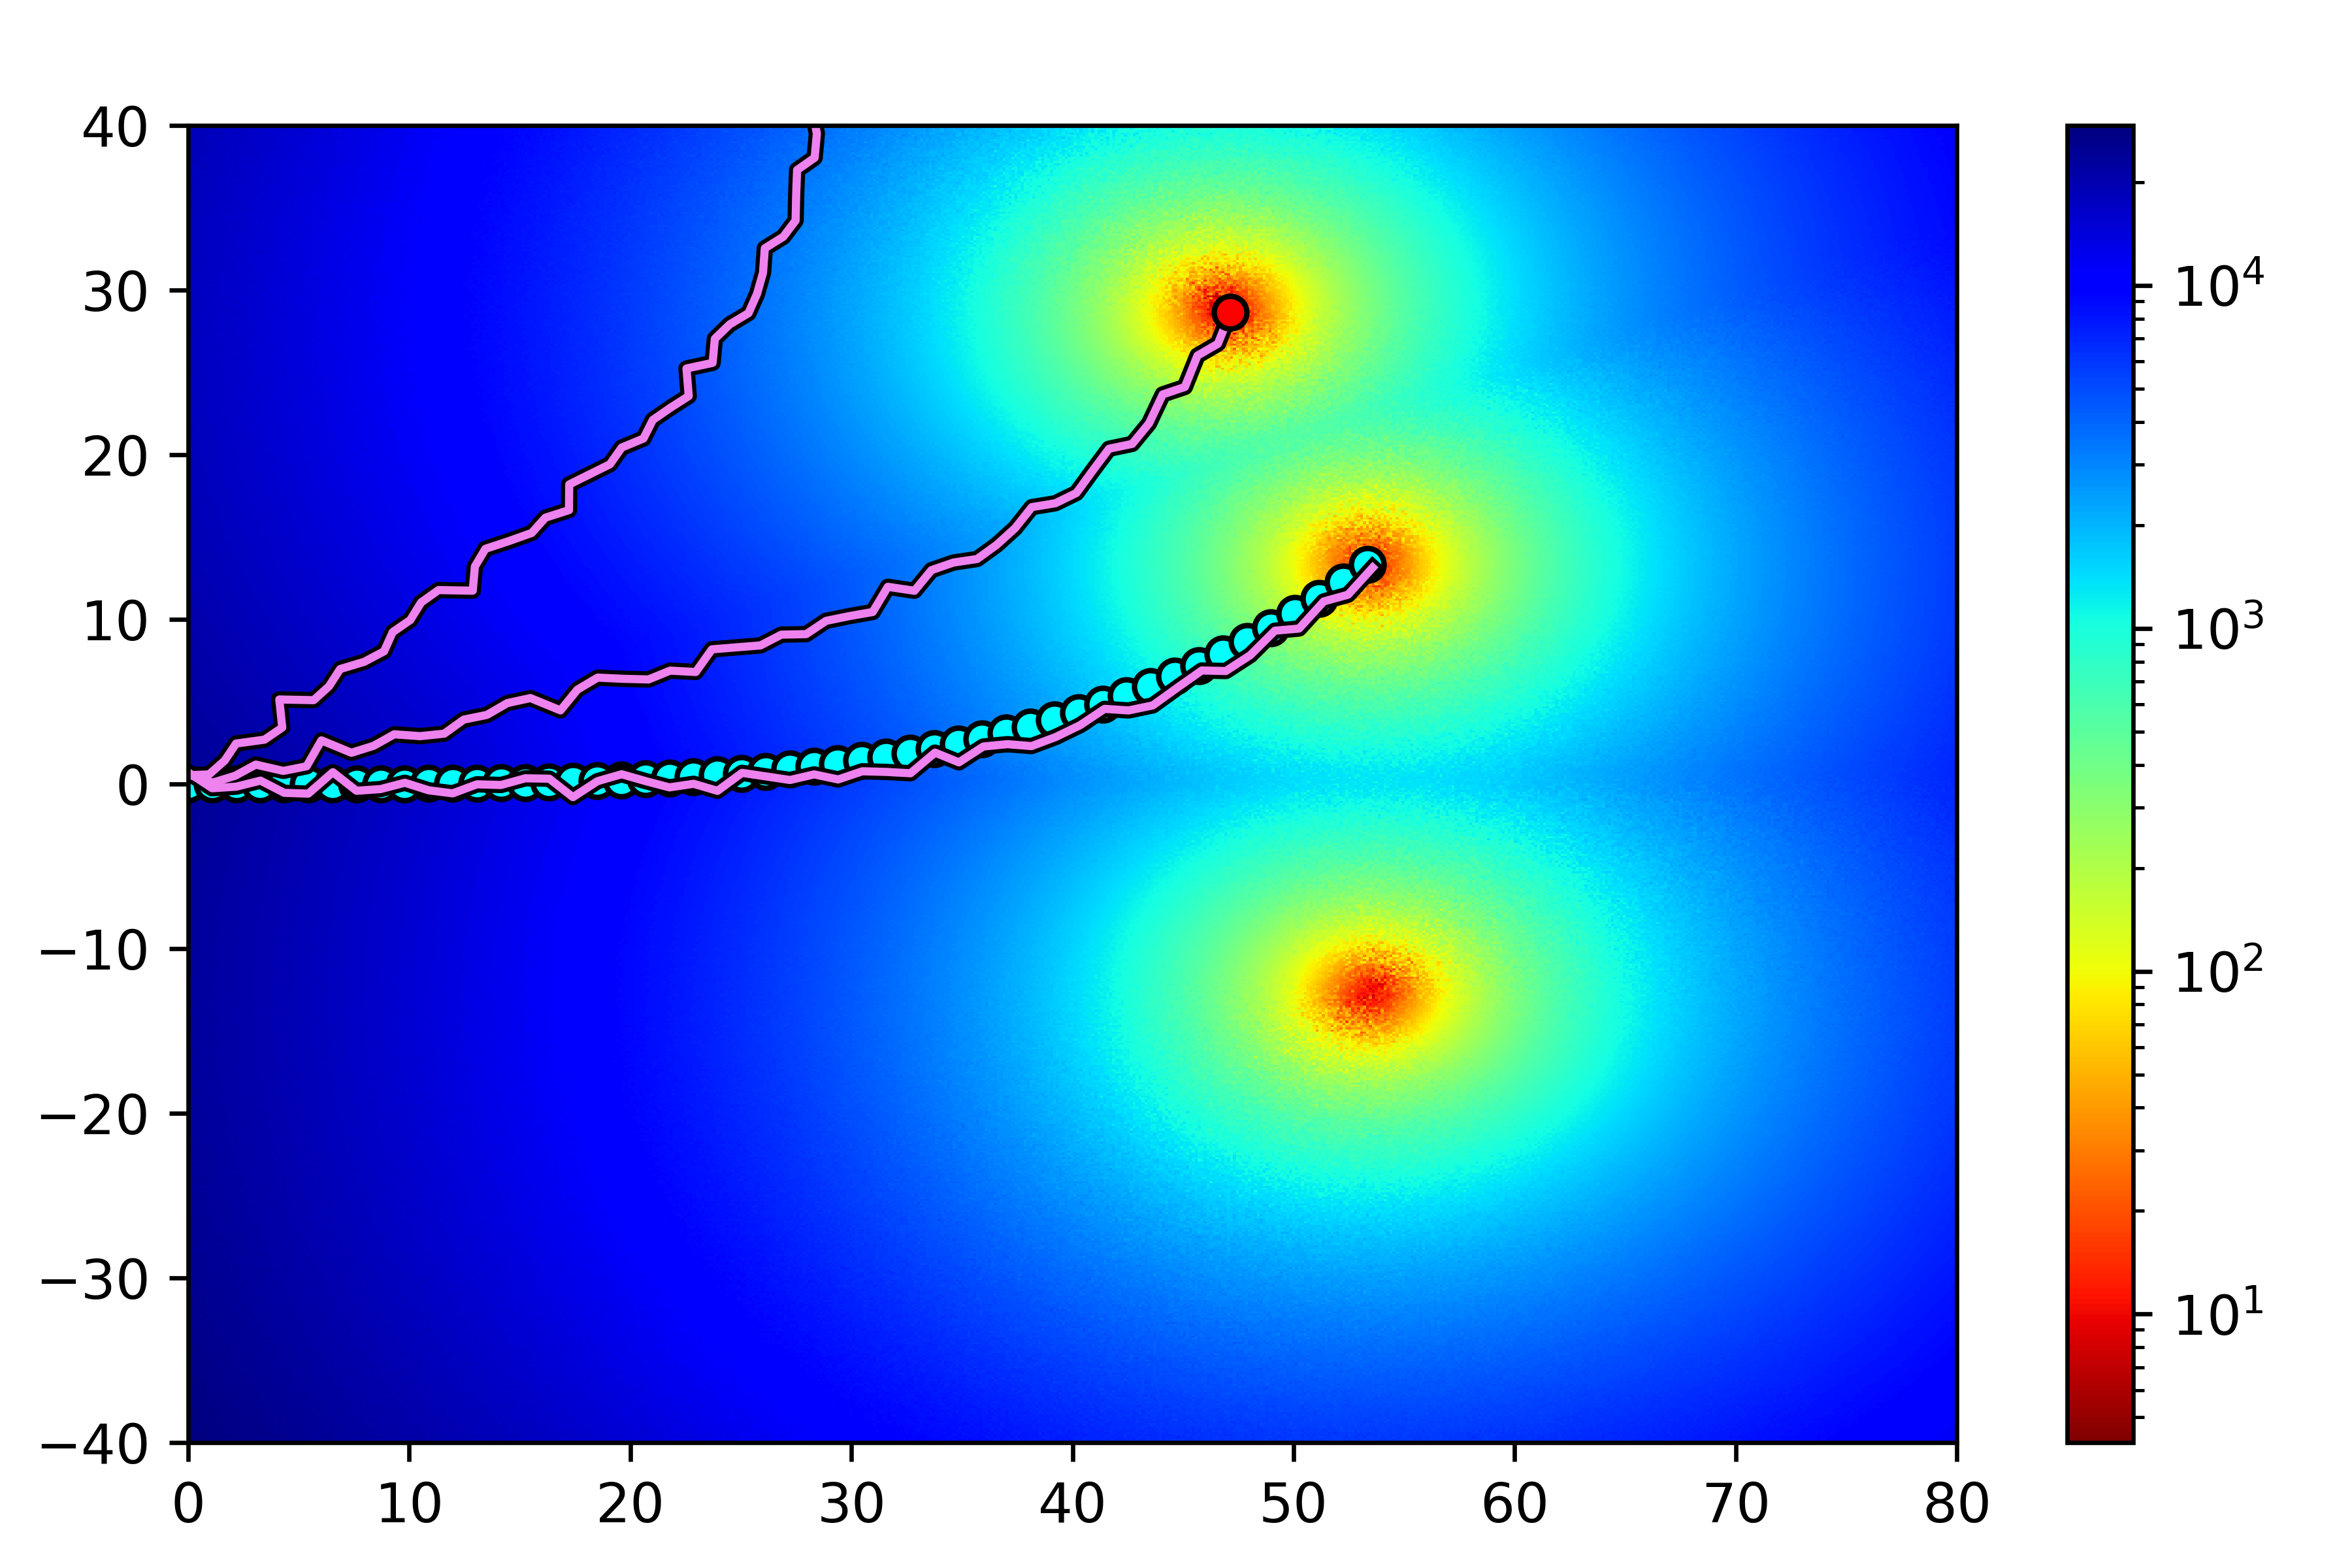
\includegraphics[width=0.5\textwidth]{loss3.png}}
\end{figure}

\begin{figure}[H]
    \centering
    \subfloat[Drugie minimum lokalne]{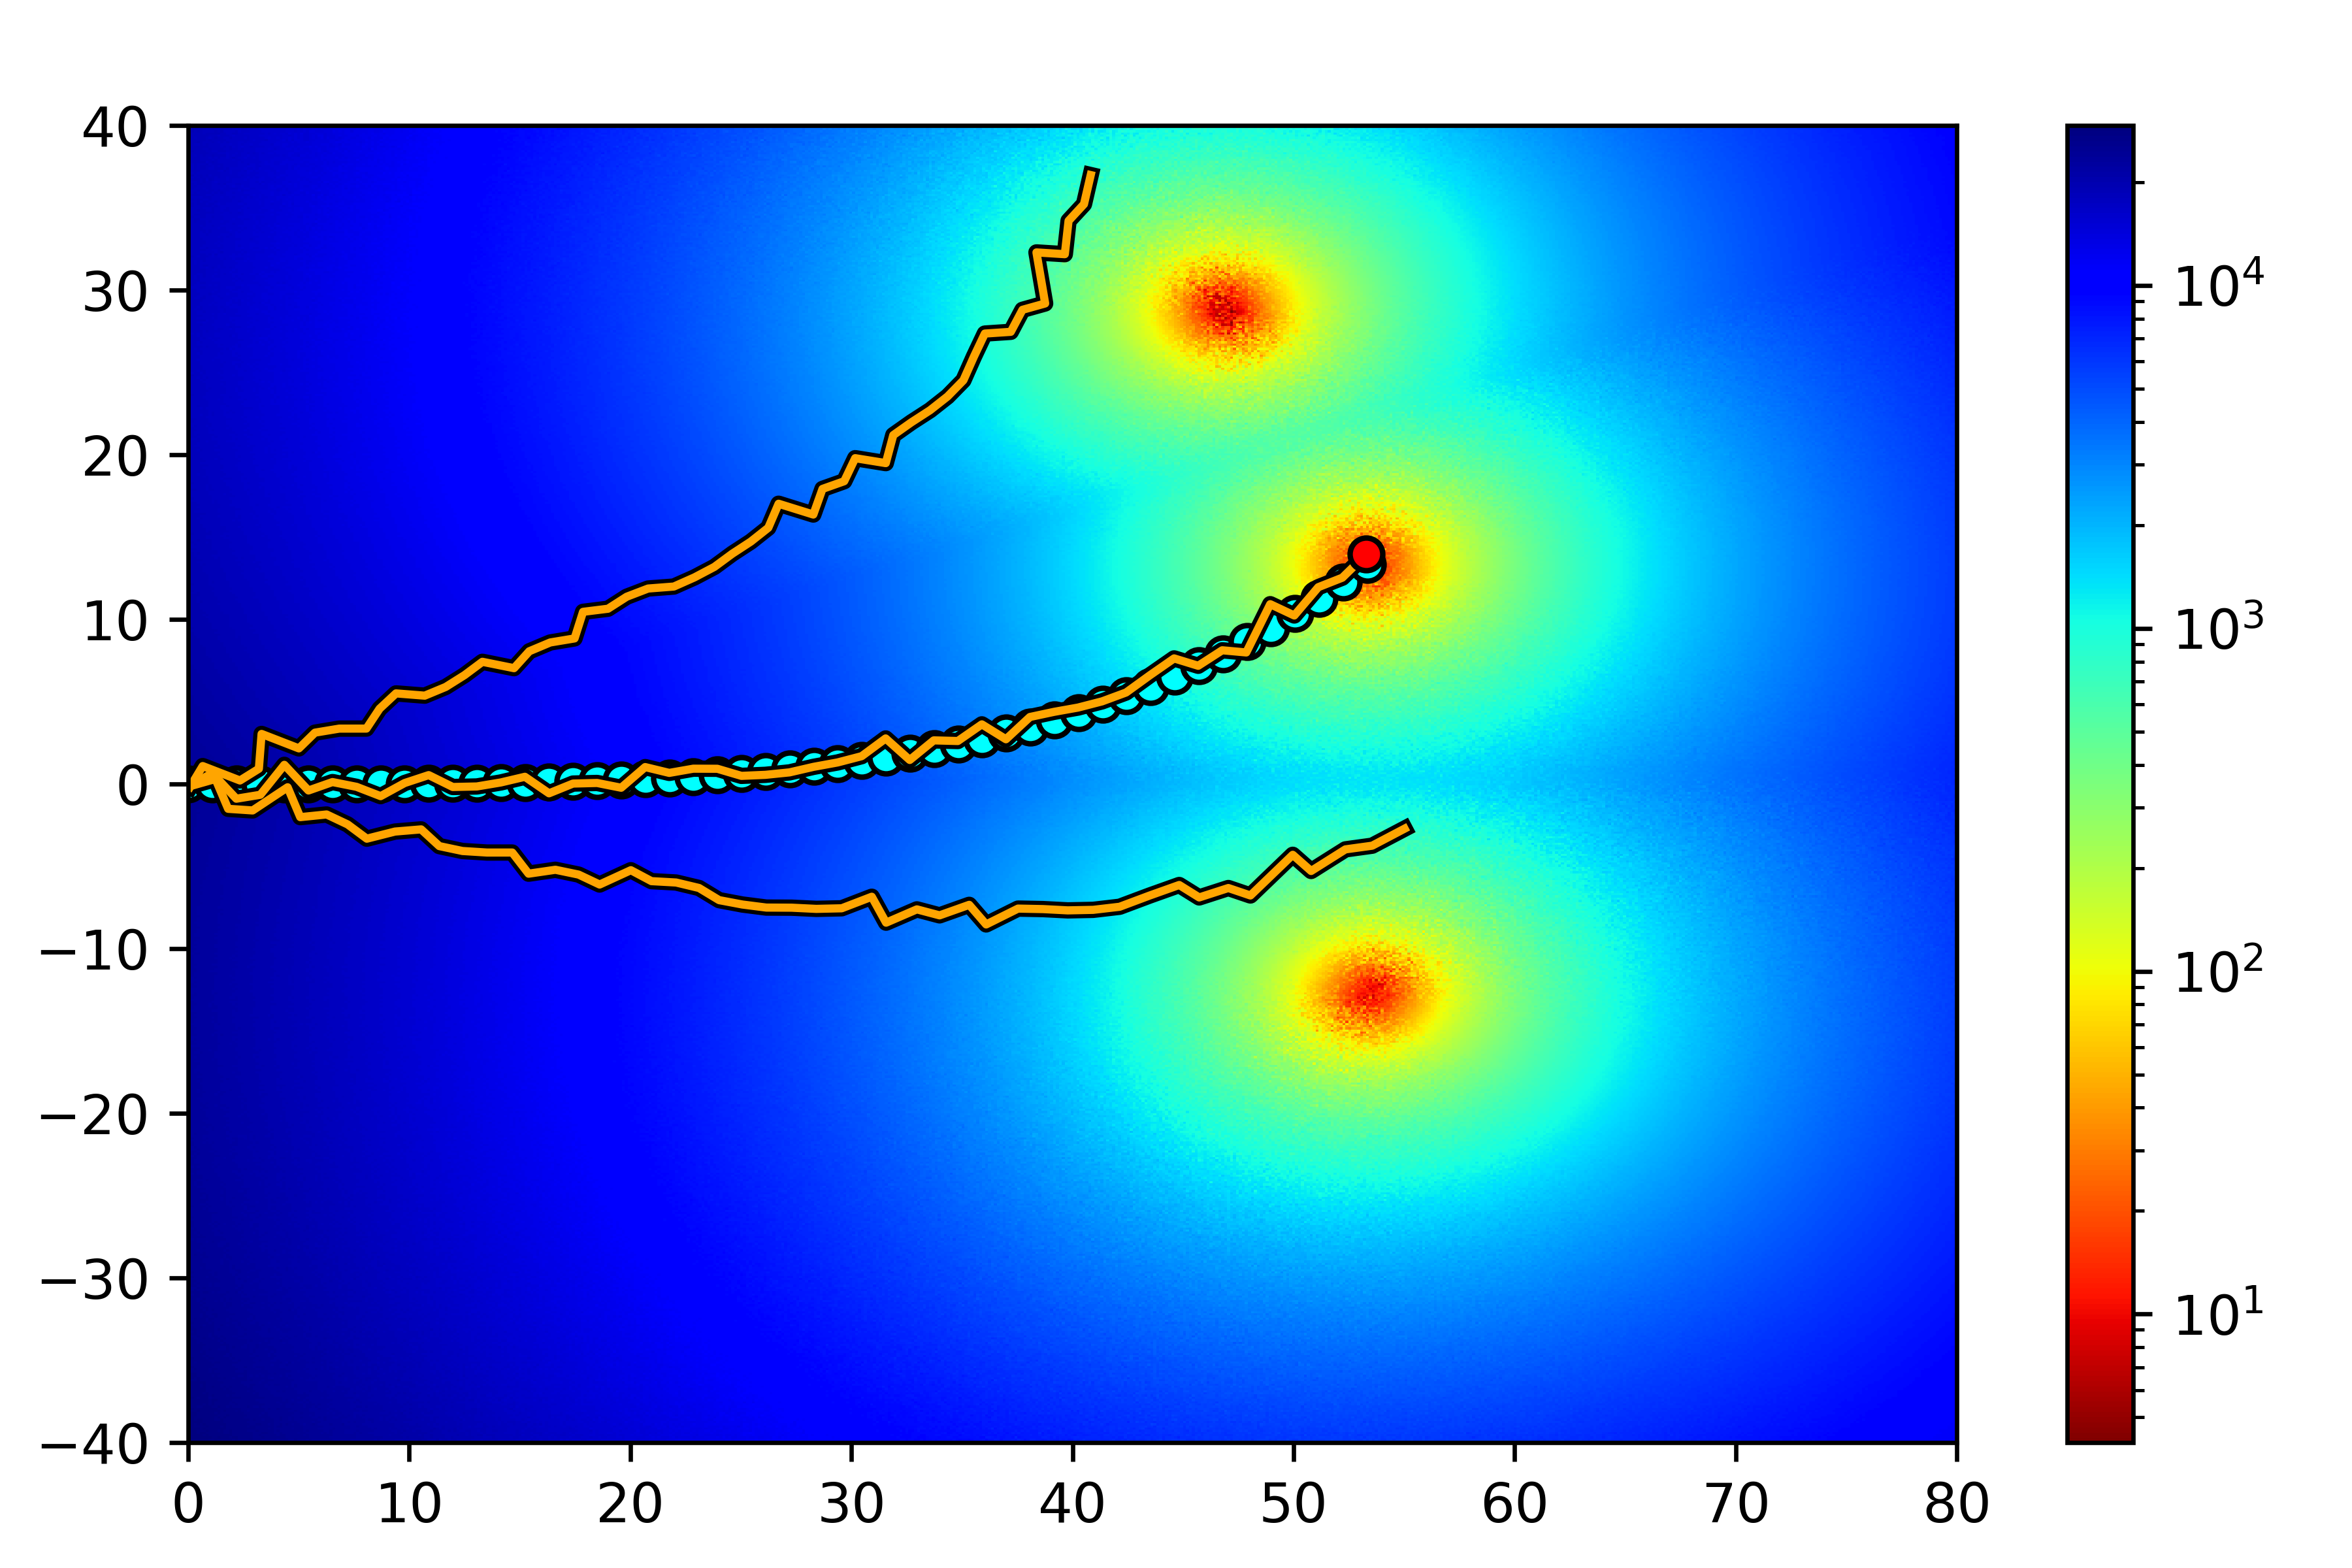
\includegraphics[width=0.5\textwidth]{loss5.png}}
    \subfloat[Trzecie minimum lokalne]{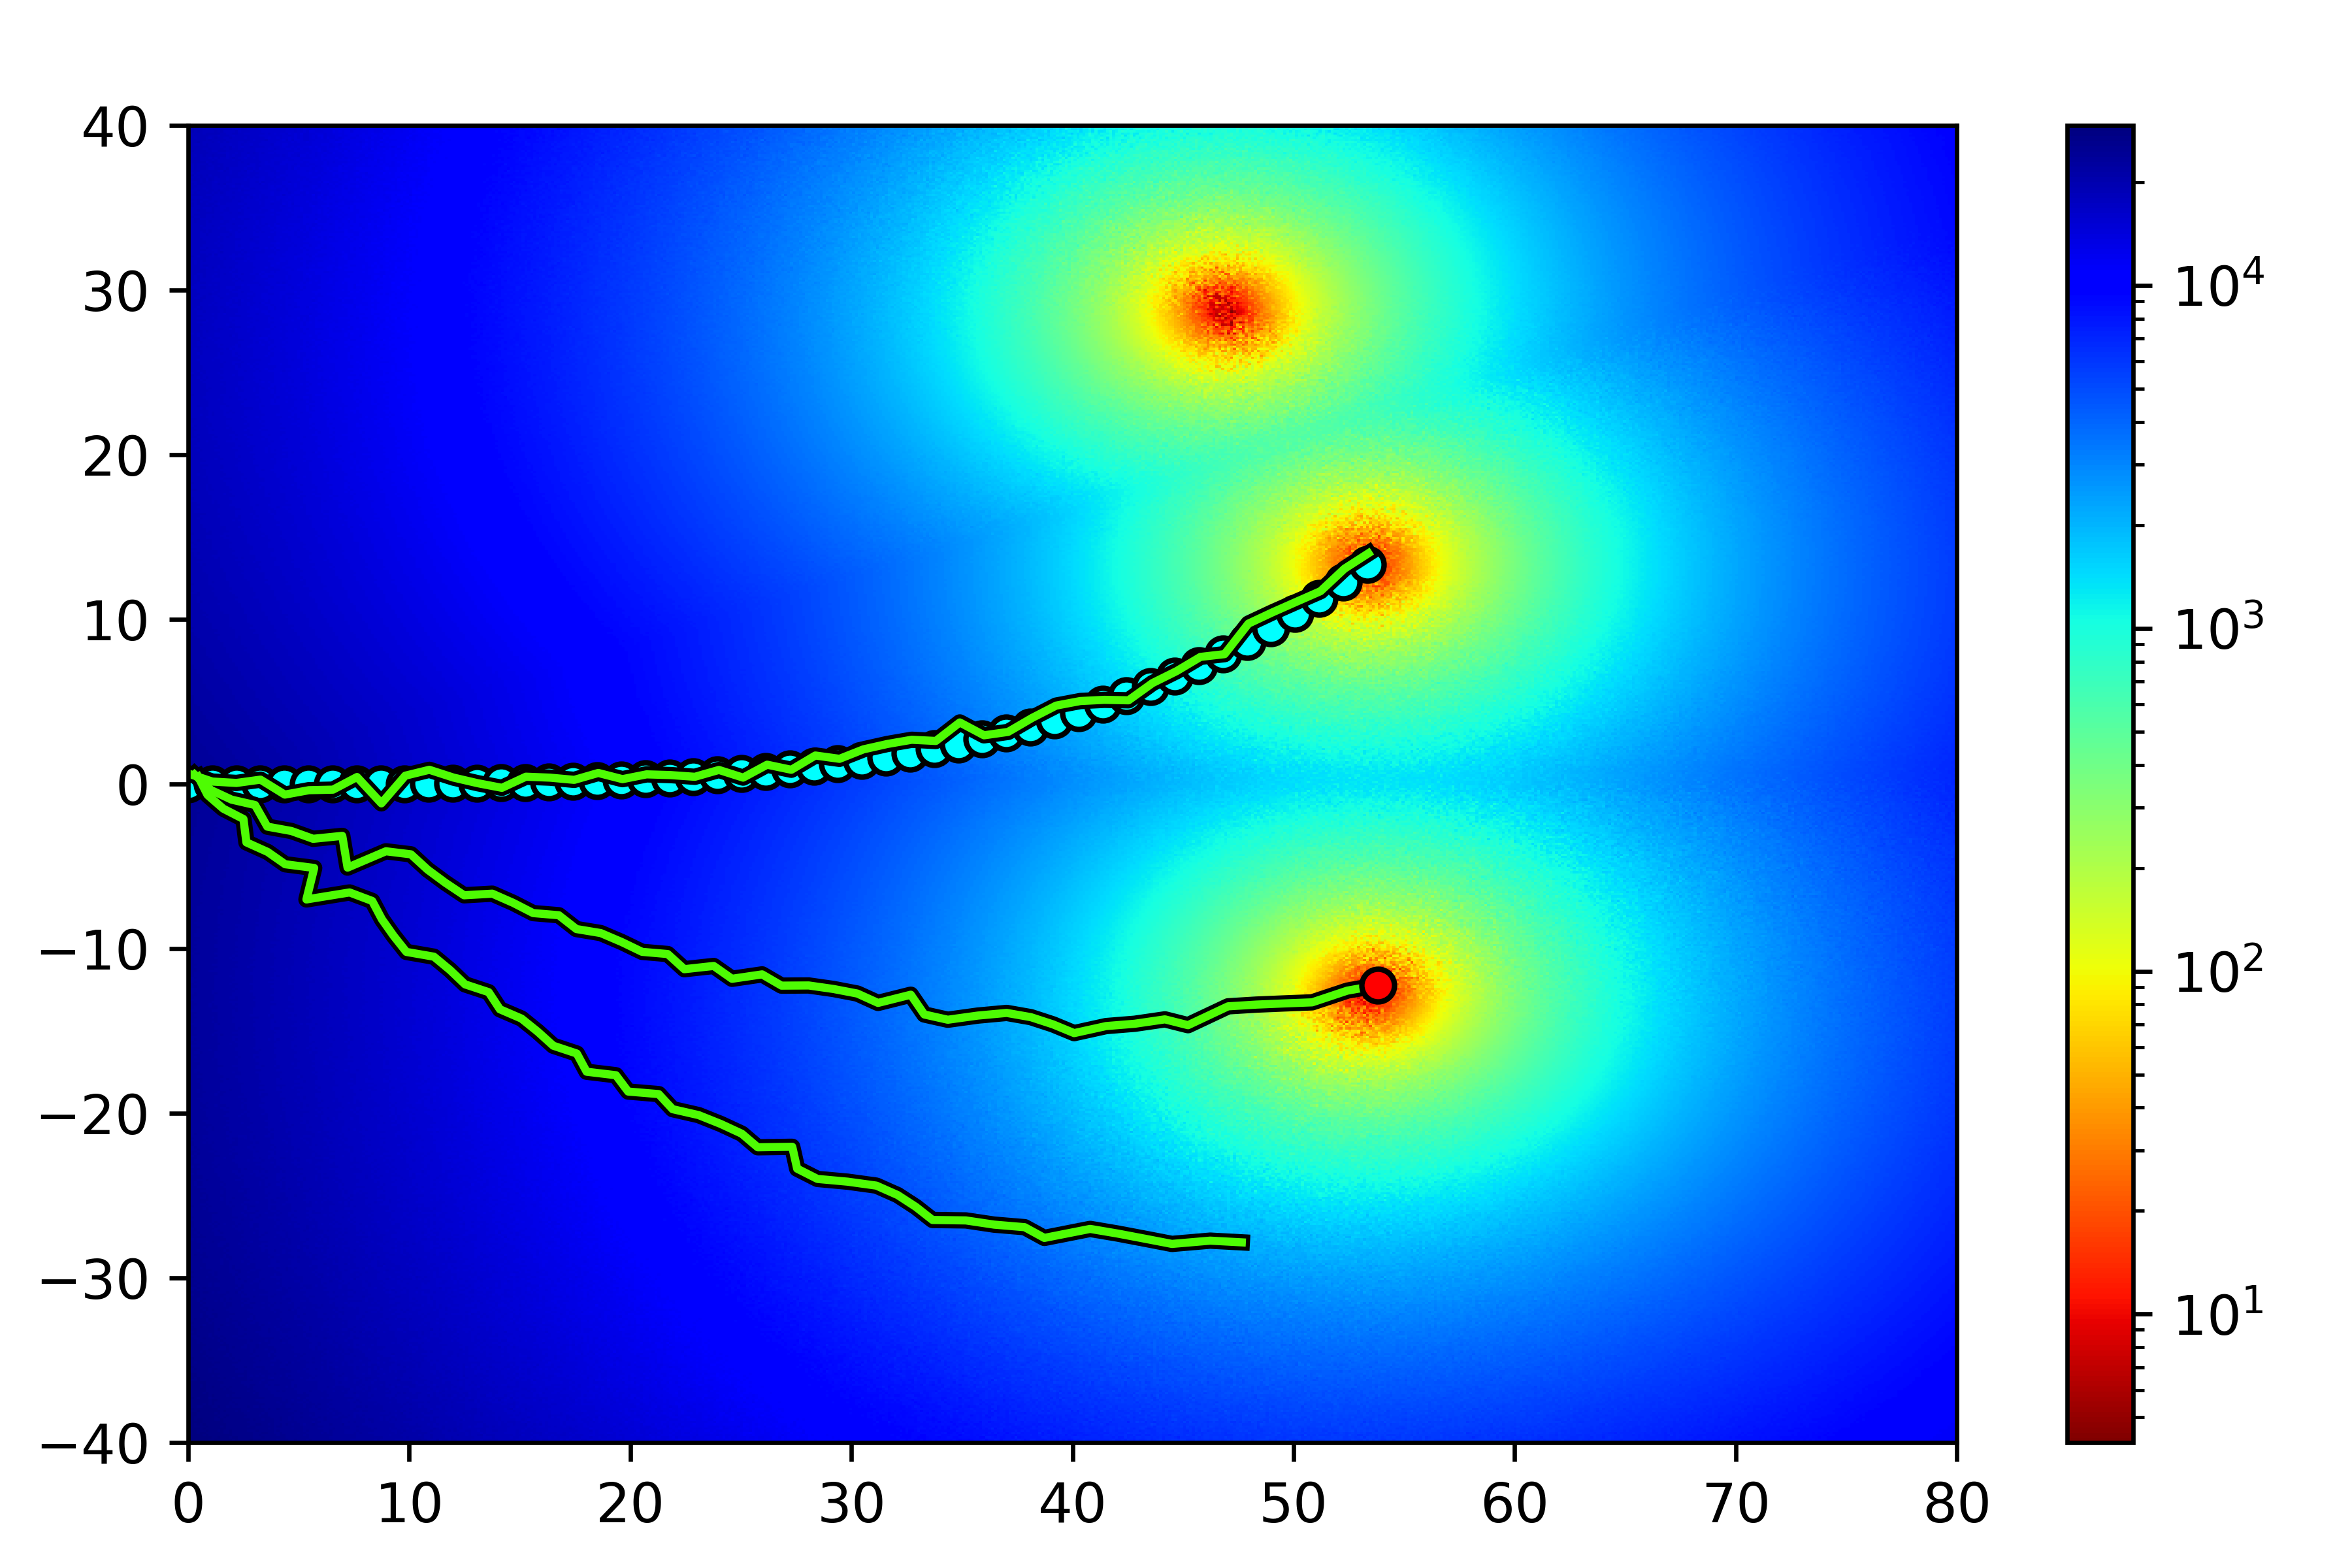
\includegraphics[width=0.5\textwidth]{loss4.png}}
\end{figure}

\newpage

\section{Opis wizualizacji}

\subsubsection{(a) Wyjściowe pozycje agenta EGO}
Na wykresie seledynowymi kropkami zaznaczono wyjściowe pozycje pewnego agenta \texttt{EGO} ze zbioru. Są to współrzędne, które nie są dostępne w chwili $t$, gdyż dotyczą następnych pięciu sekund. Przewidywanie tych współrzędnych jest zadaniem modelu predykcyjnego, który ma za zadanie zrobić to z jak największą dokładnością (ma możliwość przewidzenia trzech scenariuszy, czyli trzech trajektorii).
\subsubsection{(b) Trajektorie naśladujące predykcje modelu}
Na tym wykresie zaprezentowano pewne trzy trajektorie (uzależnione od parametru nazywanego \textit{punktem definującym trajektorie}), trajektorie te są z góry ustalone i mają za zadanie symulować działanie modelu predykcyjnego. Poniżej omówione zostanie jak trajektorie te wpływają na funkcję kosztu oraz to jak sprawić aby funkcja kosztu była jak najmniejsza. Zaproponowane trajektorie zaznaczone na czarno są uzależnione od punktu definującego trajektorie (tutaj ($x=1, y=0$)), który ustala położenie trzech trajektorii, poprzez obrót i skalowanie trajektorii bazowych (trzy czarne trajektorie). Na szaro zaznaczone zostały trajektorie bazowe obrócone i przeskalowane w wyniku zmiany położenia punktu definiującego trajektorie ($x=0.25, y=0.5$). Położenie punktu definiującego trajektorie i jego wpływ na funkcję kosztu będzie następnie analizowane za pomocą mapy ciepła (ang. heat map).
\subsubsection{(c) Wartości funkcji kosztu}
Na tym wykresie przedstawione zostały pozycje agenta \texttt{EGO} oraz mapa ciepła przedstawiająca wartość funkcji kosztu w zależności od pozycji punktu definiującego trajektorie, dla trajektorii bazowych zaproponowanych na wykresie (b). Na wykresie można zauważyć trzy minima lokalne.
\subsubsection{(d), (e), (f) Pierwsze, drugie i trzecie minimum lokalne}
Położenie minimów lokalnych, na wykresie (d), (e) i (f) nie jest przypadkowe. Minima lokalne odpowiadają takim położeniom punktu definiującego trajektorię, które sprawiają, że jedna z trajektorii pokrywa się z trajektoriami wyjściowymi agenta \texttt{EGO}. Aby uzyskać małą wartość funkcji kosztu przynajmniej jedna z trajektorii musi być zgodna z tą, która została zrealizowana (zgodna z pozycjami wyjściowymi). Gdy jedna z trzech przewidywanych trajektorii jest blisko wyjściowej trajektorii agenta \texttt{EGO}, powoduje to, że prawdopodobieństwo uzyskania obserwacji (trajektorii agenta \texttt{EGO}) z mieszaniny rozkładów normalnych, gdzie jedna z trajektorii jest blisko trajektorii agenta \texttt{EGO}, jest w pewnym sensie duże. Wtedy funkcja wiarygodności przyjmuje odpowiednio dużą wartość, a co za tym idzie funkcja kosztu odpowiednio małą wartość, gdyż na funkcję wiarygodności o odpowiednio dużej wartości jest nakładany logarytm (funkcja rosnąca) oraz ujemny znak (funkcja malejąca). Z powyższego wynika, że funkcja kosztu spełnia swoje zadanie, minimalizowanie jej w pewnym sensie zmusza model do przewidywania jednej z trzech trajektorii dostatecznie blisko pozycji wyjściowych agenta \texttt{EGO}. Można łatwo pokazać, że funkcja kosztu osiąga wartość najmniejszą równą 0 wtedy i tylko wtedy, gdy wszystkie trajektorie przewidywane przez model, które nie posiadają przewidywanego prawdopodobieństwa równego 0, dokładnie pokrywają się z pozycjami wyjściowymi agenta \texttt{EGO}.
	\cleardoublepage
	
	\chapter{Naiwna metoda rozwiązania problemu}
\thispagestyle{chapterBeginStyle}

\section{Opis}

Problem predykcji pozycji wyjściowych agenta \texttt{EGO} może być rozważany z odrzuceniem informacji dotyczących otoczenia. Przewidywanie pozycji bez wiedzy na temat obiektów w otoczeniu, pozycji pasów ruchu oraz świateł ignoruje większość użytecznych danych, które mogą zwiększyć skuteczność przewidywania możliwych scenariuszy ruchu agenta \texttt{EGO}. Opisany w tym rozdziale model ma za zadanie przede wszystkim ukazanie jaką wartość funkcji kosztu uzyskuje naiwne podejście, które wykorzystuje tylko wejściowe pozycje oraz wnioskuje pozycje wyjściowe z użyciem pewnych prostych założeń na temat ruchu agenta. Podejście to całkowicie pomija bardzo istotne aspekty ruchu takie jak zatrzymywanie się, przyśpieszanie czy oczekiwanie na zielone światło w celu ruszenia z miejsca.

\section{Model stałej prędkości}

\noindent
Załóżmy, że pozycje wejściowe agenta \texttt{EGO} są równe:

\begin{equation}
E_{t} = [(x_{0},y_{0}), (x_{1},y_{1}), ... , (x_{10},y_{10})]
\end{equation}

\noindent
Załóżmy, że pozycje wyjściowe agenta \texttt{EGO} są równe:

\begin{equation}
V_{t} = [(x_{0},y_{0}), (x_{1},y_{1}), ... , (x_{49},y_{49})]
\end{equation}

\noindent
Załóżmy, że pozycje wyjściowe agenta \texttt{EGO} spełniają założenia modelu stałej prędkości:

\begin{equation}
\exists\Delta V_{t}\:\forall i \quad V_{t}[i+1] - V_{t}[i] = \Delta V_{t}
\end{equation}

\noindent
Z takimi założeniami wektor pozycji wyjściowych ma postać:
\begin{equation}
V_{t} = [V_{t0}, V_{t0} + 1\cdot\Delta V_{t}, ... , V_{t0} + 49\cdot\Delta V_{t}]
\end{equation}

\noindent
Pozostaje jeszcze problem oszacowania $V_{t0}$ oraz $\Delta V_{t}$. Można to zrobić używając pozycji wejściowych:

\begin{equation}
\Delta V_{t} = E_{10} - E_{9}
\end{equation}

\vspace*{-5mm}

\begin{equation}
V_{t0} = E_{10} + \Delta V_{t}
\end{equation}

\vspace*{-5mm}

\section{Wyniki}
Działanie modelu zostało sprawdzone na zbiorze testowym. Uzyskane trajektorie zostały skopiowane trzy razy dla każdej próbki, dzięki czemu można było zastosować funkcję kosztu $L$. Nie było wymagane trenowanie, gdyż model ten nie posiada parametrów. Uzyskany wynik wynosi $L = 215.56$. Jest to bardzo duża wartość funkcji kosztu, co pozwala stwierdzić, że model ten bardzo źle spełnia zadanie predykcji trajektorii.
	\cleardoublepage
	
	\chapter{Głębokie sieci neuronowe}
\thispagestyle{chapterBeginStyle}

\section{Opis architektury}

Do przewidywania pozycji wyjściowych agenta \texttt{EGO} można wykorzystać głębokie sieci neuronowe. Rozważane w tej pracy sieci neuronowe składają się ze szkieletu odpowiadającego za przetwarzanie rasteryzowanych scen (głębokie sieci konwolucyjne) oraz z części składającej się z gęstych warstw odpowiadającej za dalsze przetworzenie wyjść z sieci szkieletowej na przewidywane pozycje wyjściowe agenta \texttt{EGO}.

\begin{figure}[htbp]
    \centering
    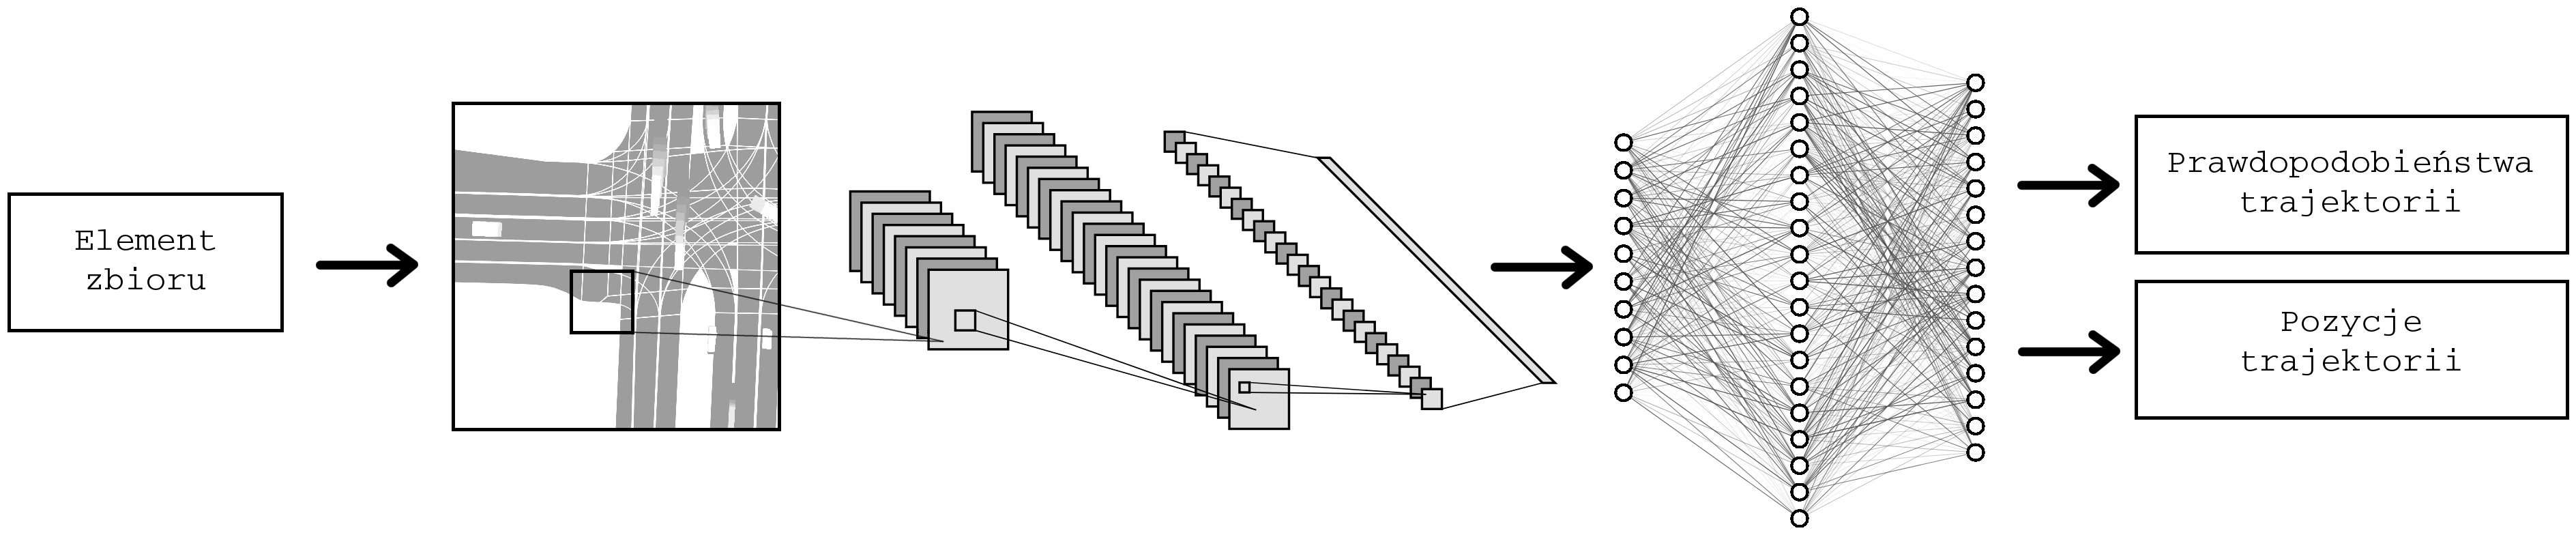
\includegraphics[width=\linewidth]{nn_schema.png}
    \caption{Wizualizacja architektury sieci neuronowej}
\end{figure}

\noindent
Proces predykcji opisanej sieci neuronowej przebiega w następujący sposób:
\begin{itemize}
    \setlength{\itemsep}{1pt}
    \setlength{\parskip}{0pt}
    \setlength{\parsep}{0pt}
    \item Ustalony zostaje indeks próbki (próbka to element zbioru).
    \item Wczytane zostają wszystkie dane dotyczące próbki (agenci, pasy, światła itd.)
    \item Następuje rasteryzacja próbki (stworzenie podglądu sceny)
    \item Otrzymany obraz jest przetwarzany przez szkielet sieci (część składająca się z warstw konwolucyjnych).
    \item Wektor cech podawany jest na wejście gęsto połączonej sieci neuronowej. Sieć ta zwraca wektor posiadający prawdopodobieństwa trajektorii i pozycje przewidywanych trajektorii.
\end{itemize}

\noindent
Szkielet sieci domyślnie przyjmuje obrazy o wymiarach $(3, H, W)$, lecz rasteryzator \texttt{SemBoxRasterizer} zwraca obrazy o wymiarach $(25, H, W)$, gdzie kanały posiadają następujące informacje:

\begin{itemize}
    \setlength{\itemsep}{1pt}
    \setlength{\parskip}{0pt}
    \setlength{\parsep}{0pt}
    \item 0-11 zawierają zaznaczone wejściowe pozycje agenta \texttt{EGO} w chwilach \mbox{$[t, t-0.1, ... , t-1.0]$}
    \item 11-22 zawierają zaznaczone wejściowe pozycje agentów innych niż \texttt{EGO} w chwilach \mbox{$[t, t-0.1, ... , t-1.0]$}
    \item 23-25 zawierają rasteryzowaną scenę w formacie RGB (wszystkie informacje agenci, pasy, światła itd.)
\end{itemize}

Z tego powodu wymagana jest modyfikacja pierwszej warstwy konwolucyjnej w domyślnych sieciach szkieletowych. Pierwsza warstwa konwolucyjna jest usuwana i zastępowana jest warstwą o tych samych argumentach (padding, stride itp), z wyjątkiem liczby kanałów wejściowych, która zamieniana jest z 3 na 25. Trzeba zaznaczyć, że wykonywane jest to tylko przy korzystaniu z rasteryzatora \texttt{SemBoxRasterizer}, w przypadku rasteryzatora \texttt{CenterLines} pierwsza warstwa konwolucyjna nie jest modyfikowana, gdyż rasteryzator ten zwraca obraz z trzema kanałami.

\newpage

\subsection{Szczegółowy opis warstw sieci}

\begin{itemize}
    \setlength{\itemsep}{1pt}
    \setlength{\parskip}{0pt}
    \setlength{\parsep}{0pt}
    \item Szkielet sieci przyjmuje obraz o wymiarach $(3, H, W)$ lub $(25, H, W)$
    \item Szkielet sieci zwraca wektor długości \texttt{backbone\_out\_features} w zależności od użytego typu sieci:
        \begin{itemize}
            \setlength{\itemsep}{1pt}
            \setlength{\parskip}{0pt}
            \setlength{\parsep}{0pt}
            \item \texttt{ResNet-18}: 512
            \item \texttt{ResNet-34}: 512
            \item \texttt{ResNet-50}: 2048
            \item \texttt{EfficientNet-B3}: 1536
            \item \texttt{EfficientNet-B5}: 2048
            \item \texttt{EfficientNet-B6}: 2304
            \item \texttt{MixNet-M}: 1536
            \item \texttt{MixNet-L}: 1536
        \end{itemize}
    \item Warstwa głęboko połączona przyjmuje wektor długości \texttt{backbone\_out\_features}, zwraca wektor długości 4096. Nakładana jest funkcja aktywacji \texttt{ReLU}.
    \item Warstwa głęboko połączona przyjmuje wektor długości 4096, zwraca wektor długości 303 odpowiadający elementom tensora zawierającego 3 trajektorie (w 2 wymiarach: x oraz y) i 3 prawdopodobieństwa trajektorii. Stąd $303 = 3*(50 * 2 + 1)$
\end{itemize}

\section{Szkielet sieci neuronowej}

\subsection{Ogólne porównanie}

\begin{center}
\begin{tabular}{ |c|c|c|c|c| } 
\hline
Nazwa sieci & Data opublikowania & Liczba parametrów & ImageNet błąd Top1 & ImageNet błąd Top5\\
\hline
ResNet-18 & 10.12.2015r. & 11.2 mln & 30.2 & 10.9\\
\hline
ResNet-34 & 10.12.2015r. & 21.3 mln & 26.7 & 8.6\\
\hline
ResNet-50 & 10.12.2015r. & 23.6 mln & 23.9 & 7.1\\
\hline
EfficientNet-B3 & 28.05.2019r. & 12.0 mln & 18.4 & 4.3\\
\hline
EfficientNet-B5 & 28.05.2019r. & 30.0 mln & 16.4 & 3.3\\
\hline
EfficientNet-B6 & 28.05.2019r. & 43.0 mln & 16.0 & 3.2\\
\hline
MixNet-M & 22.07.2019r. & 5.0 mln & 23.0 & 6.7\\
\hline
MixNet-L & 22.07.2019r. & 7.3 mln & 21.1 & 5.8\\
\hline
\end{tabular}
\end{center}

\subsection{\texttt{ResNet}}
Głębokie sieci neuronowe bywają trudne w trenowaniu, często wynika to z efektu zanikających oraz eksplodujących gradientów. Architektura \texttt{ResNet} \cite{1512.03385} była jednym z pierwszych udanych rozwiązań tego problemu w odniesieniu do problemów wizji z użyciem sieci \texttt{CNN} (sieci konwolucyjnych). Pozwoliło to na zwiększenie głębokości sieci neuronowych, co przyczyniło się do polepszenia skuteczności sieci \texttt{CNN}. Obecnie istnieje wiele lepszych architektur sieci  \texttt{CNN} pod względem wyników na zbiorach porównawczych takich jak np. \texttt{ImageNet} \cite{deng2009imagenet}, mimo to sieci \texttt{ResNet} dalej są wykorzystywane ze względu na bardzo dobry kompromis pomiędzy skomplikowaniem architektury, a skutecznością.

\newpage

\subsection{\texttt{EfficientNet}}
Bardzo często architektury sieci neuronowych są projektowane z myślą o ograniczeniach zasobów obliczeniowych (szybkość predykcji oraz zapotrzebowanie na pamięć \texttt{RAM}). Sieci o architekturze \texttt{EfficientNet} \cite{1905.11946} zostały zaprojektowane z myślą o jak najlepszym wykorzystaniu dostępnych zasobów. Wykorzystują obserwację dotyczącą skalowania sieci, która pozwala na efektywne wykorzystanie zasobów. Powiększanie sieci w celu uzyskania lepszej jakości predykcji odbywa się nie tylko względem głębokości sieci (dodawanie kolejnych warstw konwolucyjnych). Autorzy architektury \texttt{EfficientNet} pokazali technikę, która pozwala na skalowanie głębokości, szerokości oraz rozdzielczości sieci w optymalny sposób, przy ograniczeniach na liczbę operacji zmiennoprzecinkowych na sekundę oraz używanej pamięci \texttt{RAM}. Otrzymane architektury zostały znalezione za pomocą przeszukiwania przestrzeni sieci neuronowych techniką \texttt{NAS} (ang. neural architecture search).

\subsection{\texttt{MixNet}}
Sieci konwolucyjne zazwyczaj wykorzystują konwolucję \texttt{Depthwise}, jest to typ konwolucji, której jądro obliczane jest z wykorzystaniem wszystkich kanałów jednocześnie (w odpowiednich obszarach każdego z kanałów). Sieci architektury \texttt{MixNet} \cite{1907.09595} zostały zaprojektowane z zamiarem wykorzystania wielu rozmiarów jądra konwolucji bez zbędnego zwiększania liczby parametrów sieci. Zaproponowany został w tym celu rodzaj konwolucji \texttt{MixConv}, który wykorzystuje jednocześnie wiele rozmiarów jądra w jednej konwolucji. Konwolucja \texttt{MixConv} została dodana jako jedna z opcji przy przeszukiwaniu przestrzeni sieci neuronowych techniką \texttt{NAS}. Otrzymane w wyniku przeszukiwania architektury należą do rodziny \texttt{MixNet} i wykorzystują konwolucje \texttt{MixConv}.

\section{Pretrenowanie sieci}
Opisane powyżej architektury szkieletów głębokich sieci konwolucyjnych są bardzo czasochłonne w trenowaniu. Z tego względu przy wykorzystaniu tych szkieletów do zadań wizji, wykorzystuje się tzw. pretrenowanie (ang. pre-training) \cite{1901.09960}. Jest to proces polegający na trenowaniu sieci na podobnym zbiorze do zbioru docelowego (tego, który wykorzystany zostanie do nauczenia konkretnego zadania). Najczęściej pretrenowanie odbywa się na zbiorze \texttt{ImageNet}, sieć trenowana jest na zadaniu klasyfikacji jednej z tysiąca klas obiektów obecnych w zbiorze. Na końcu pretrenowania usuwa się ostatnią warstwę sieci (głęboko połączona warstwa odpowiedzialna za klasyfikację). Dzięki temu procesowi uzyskana sieć potrafi rozróżniać kształty, kolory oraz podstawowe obiekty. Następnie wystarczy dokończyć proces trenowania na zadaniu, które rozpatrujemy. Proces pretrenowania ma za zadanie oszczędzić czas potrzebny na wyuczenie sieci podstawowych informacji o strukturze danych wejściowych (w tym wypadku obrazy). W tej pracy każdy wykorzystany szkielet został poddany procesowi pretrenowania, parametry tych sieci są pobierane z biblioteki \texttt{torchvision}. Parametrami tymi inicjalizuje się odpowiednie architektury sieci neuronowych.
	\cleardoublepage
	
	\chapter{Proces trenowania sieci neuronowych}
\thispagestyle{chapterBeginStyle}

\section{Opis procesu trenowania}

Trenowanie sieci neuronowej składa się z cyklicznych operacji, które mają za zadanie minimalizować funkcję kosztu. W każdym cyklu należy wybrać element zbioru treningowego, uzyskać predykcje modelu, obliczyć gradienty funkcji kosztu względem parametrów modelu oraz dokonać odpowiednich zmian w parametrach. Ważne jest monitorowanie zmian funkcji kosztu na zbiorze walidacyjnym (zbiór rozłączny z treningowym). Algorytm zmieniania parametrów sieci określony jest mianem optymalizatora. Poniżej opisany jest pseudokod algorytmu \texttt{train\_models}, który ma za zadanie przeprowadzić proces trenowania sieci neuronowych.

\section{Pseudokod algorytmu \texttt{train\_models}}

\begin{pseudokod}[H]
    \SetAlgoLined
    \DontPrintSemicolon
    \textbf{Dane wejściowe:} $nn\_architectures$\Comment*[r]{Lista zawierająca opisy architektur poszczególnych sieci neuronowych}
    
    \BlankLine
    $models \leftarrow \lbrack \rbrack$\;
    $train\_data\_loader \leftarrow init\_tr\_dl(batch=16)$\Comment*[r]{Obiekt zwracający podzbiory (mocy = 16) zbioru treningowego}
    $valid\_data\_loader \leftarrow init\_vl\_dl(batch=16)$\Comment*[r]{Obiekt zwracający podzbiory (mocy = 16) zbioru walidacyjnego}
    
    \BlankLine
    \For{$nn\_architecture$ $\in$ $nn\_architectures$}{
        $nn \leftarrow init\_nn(nn\_architecture)$\Comment*[r]{Inicjalizacja sieci zgodnie z opisem architektury}
        $models.append(nn)$\;
    }
    
    \BlankLine
    \Do{process\_not\_killed}{
        $tr\_batch \leftarrow train\_data\_loader.get\_batch()$\Comment*[r]{Pozyskanie 16 elementów zbioru treningowego}
        
        \BlankLine
        \For{$nn$ $\in$ $models$}{
            $pred\_y \leftarrow nn.predict(tr\_batch)$\Comment*[r]{Wykonanie 16 predykcji dla 16 elementów zbioru treningowego}
            $tr\_loss \leftarrow L(tr\_batch.y, pred\_y)$\Comment*[r]{Obliczenie średniej wartości funkcji kosztu dla 16 elementów}
            $grad \leftarrow get\_gradients(tr\_loss)$\Comment*[r]{Gradienty uśrednionej funkcji kosztu (na 16 elementach)}
            $nn.optimizer.update\_parameters(grad)$\Comment*[r]{Wykonanie aktualizacji parametrów przez optymalizator}
            
            \BlankLine
            \uIf{$mod(tr\_batch.num, 5000) == 0$\Comment*[r]{Co 5 tys. iteracji trenujących, wykonuje się walidację modelu}}{
                $vl\_loss\_list \leftarrow \lbrack \rbrack$\;
                \BlankLine
                
                \For{$vl\_batch$ $\in$ $valid\_data\_loader$}{
                $pred\_y \leftarrow nn.predict(vl\_batch)$\Comment*[r]{Wykonanie predykcji dla każdego podzbioru }
                $vl\_loss\_list.append(L(vl\_batch.y, pred\_y))$\Comment*[r]{Średnia wartość funkcji kosztu dla 16 elementów}
                }
                
                \BlankLine
                print(vl\_loss\_list.mean())\Comment*[r]{Wypisujemy średnią wartość funkcji kosztu na zbiorze walidacyjnym}
            }
        }
        \BlankLine
    }
    
    \caption{Algorytm train\_models}
\end{pseudokod}

\newpage

\section{Wizualizacja procesu trenowania}
\subsection{Z użyciem rasteryzatora \texttt{SemBoxRasterizer}}
\begin{figure}[h!]
    \centering
    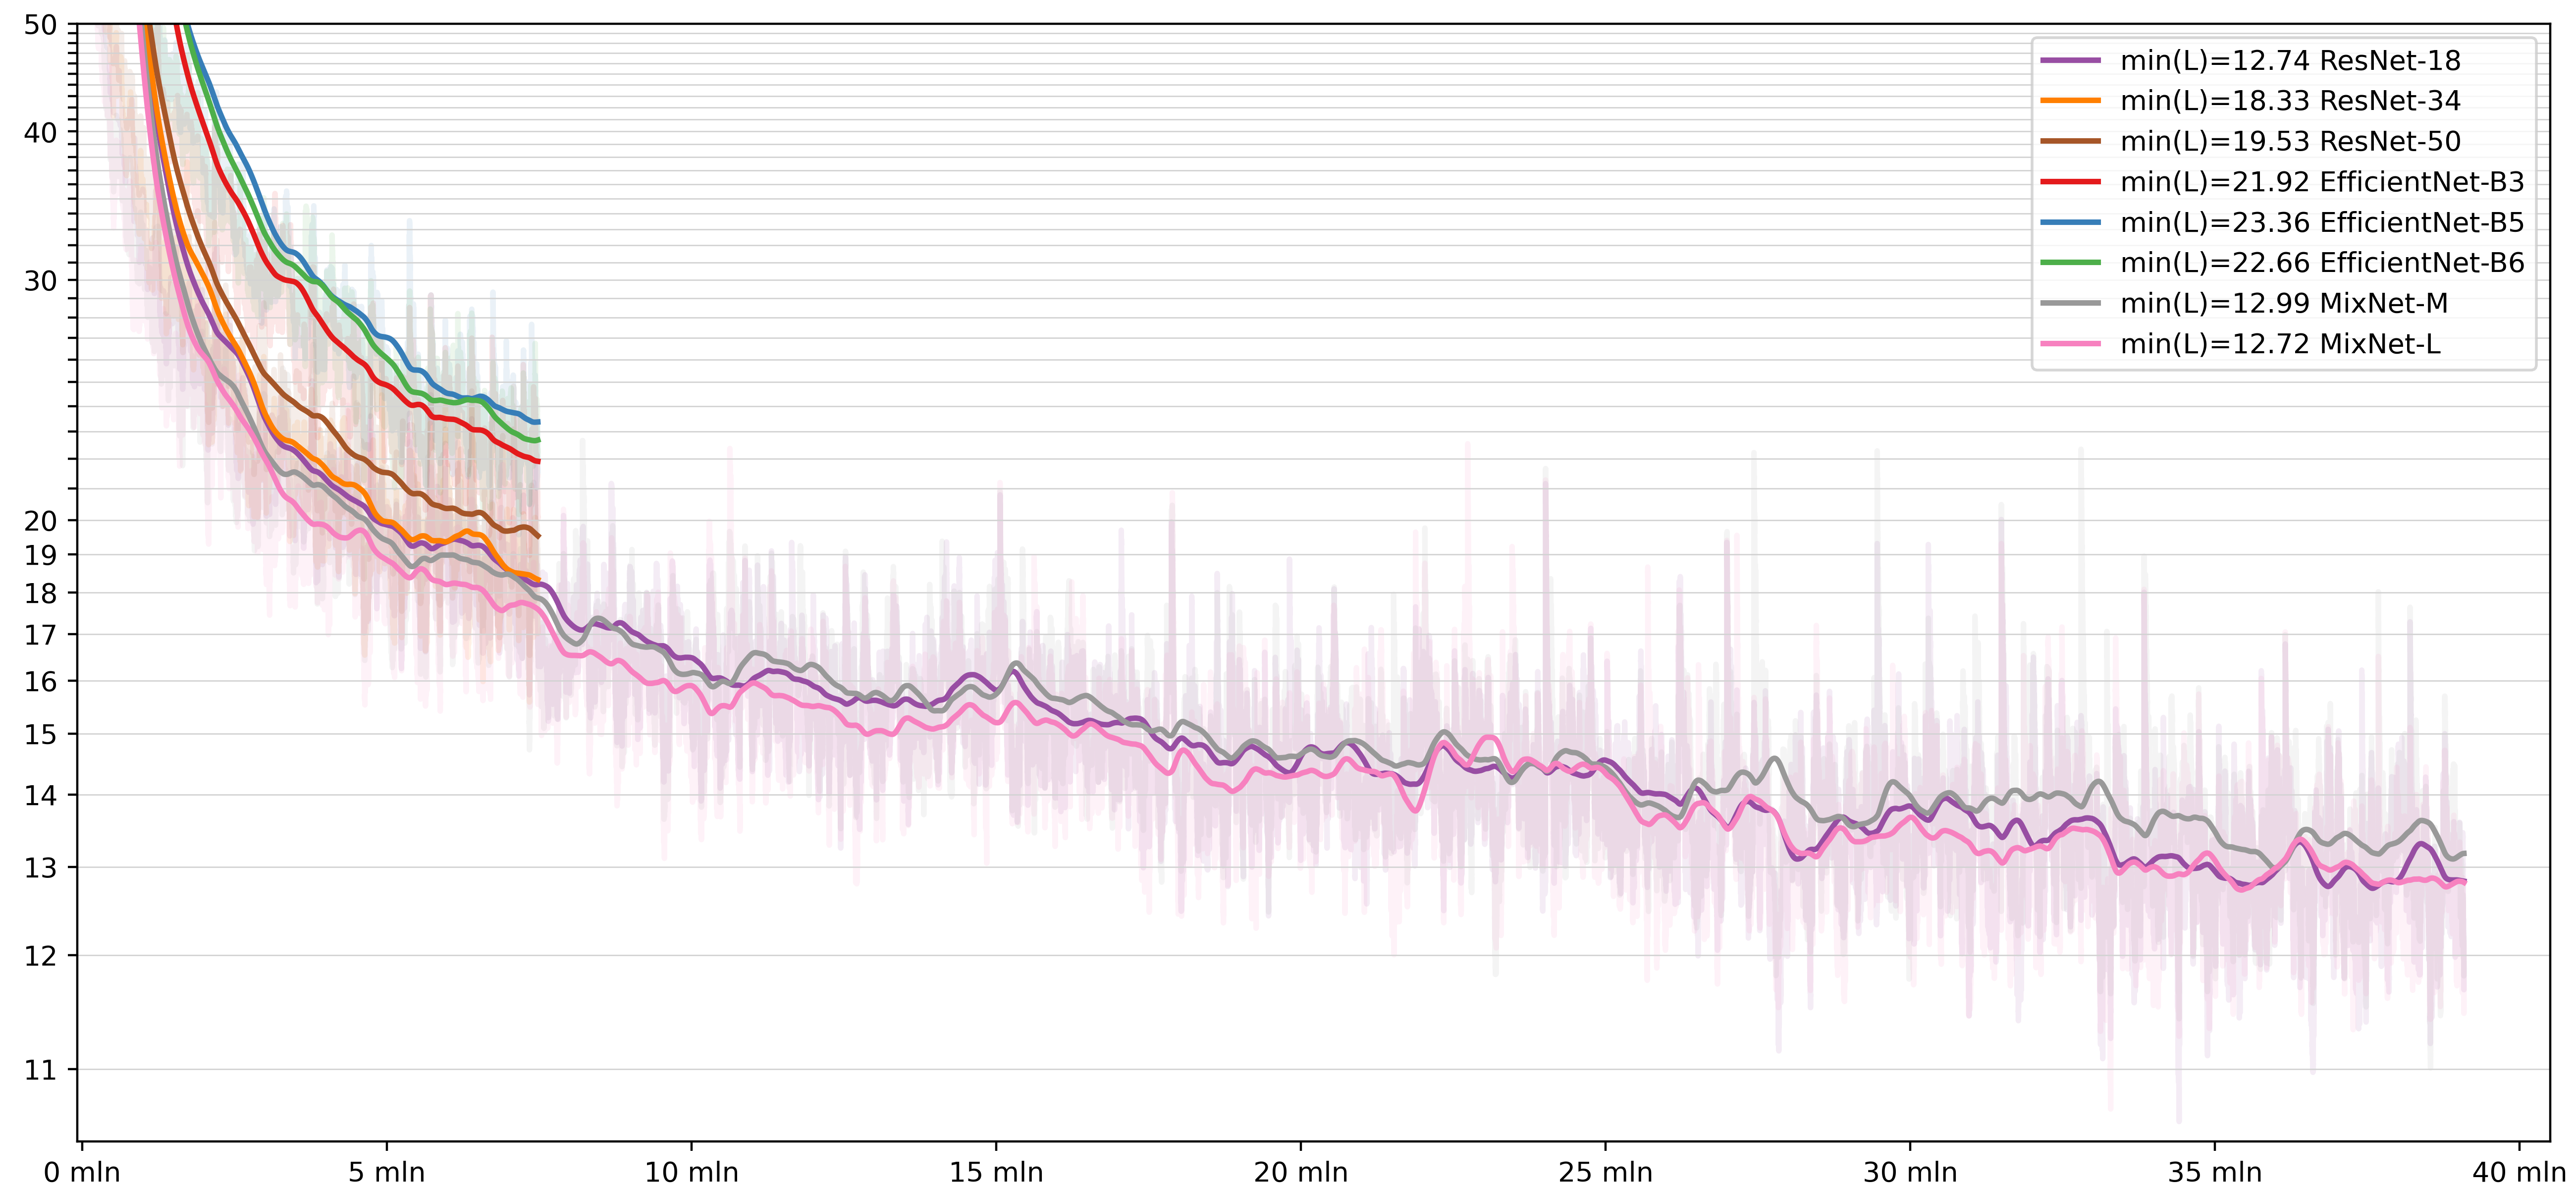
\includegraphics[width=\linewidth]{loss_sembox_train.png}
    \caption{Wartości funkcji $L$ dla próbek ze zbioru \textbf{treningowego} (wartości najmniejsze podane są dla krzywych uzyskanych z wygładzenia wykładniczego wartości funkcji $L$)}
    \vspace*{1cm}
    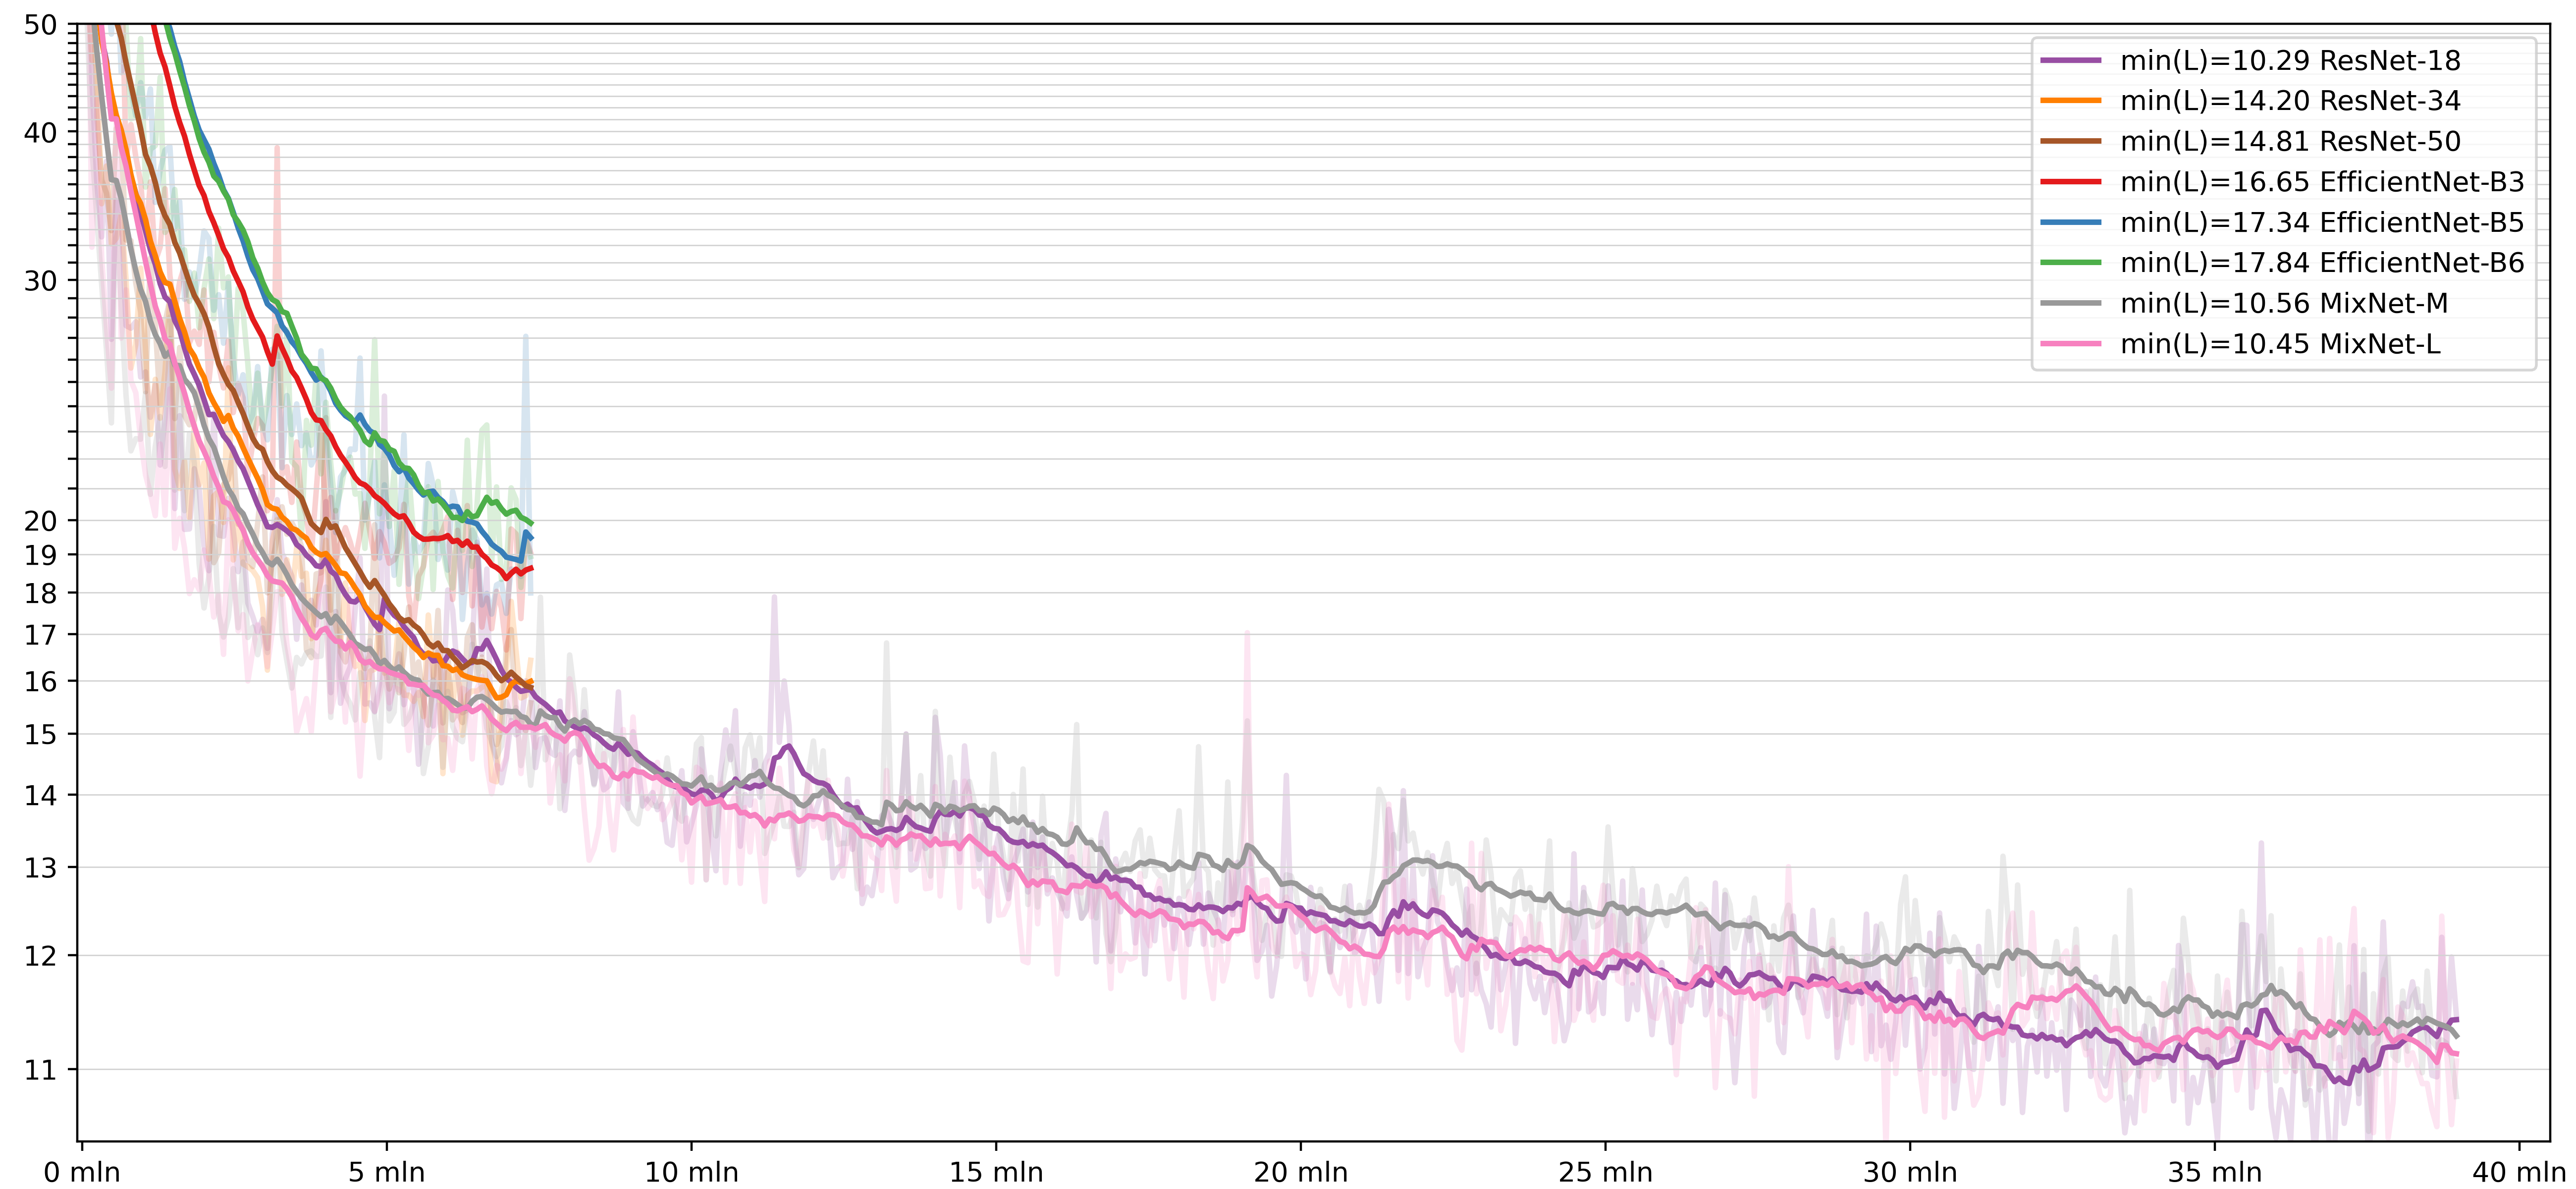
\includegraphics[width=\linewidth]{loss_sembox_val.png}
    \caption{Wartości funkcji $L$ dla próbek ze zbioru \textbf{walidacyjnego} (wartości najmniejsze podane są dla dokładnych wartości funkcji $L$)}
\end{figure}

\newpage

\subsection{Z użyciem rasteryzatora \texttt{CenterLines}}
\vspace*{0cm}

\begin{figure}[h!]
    \centering
    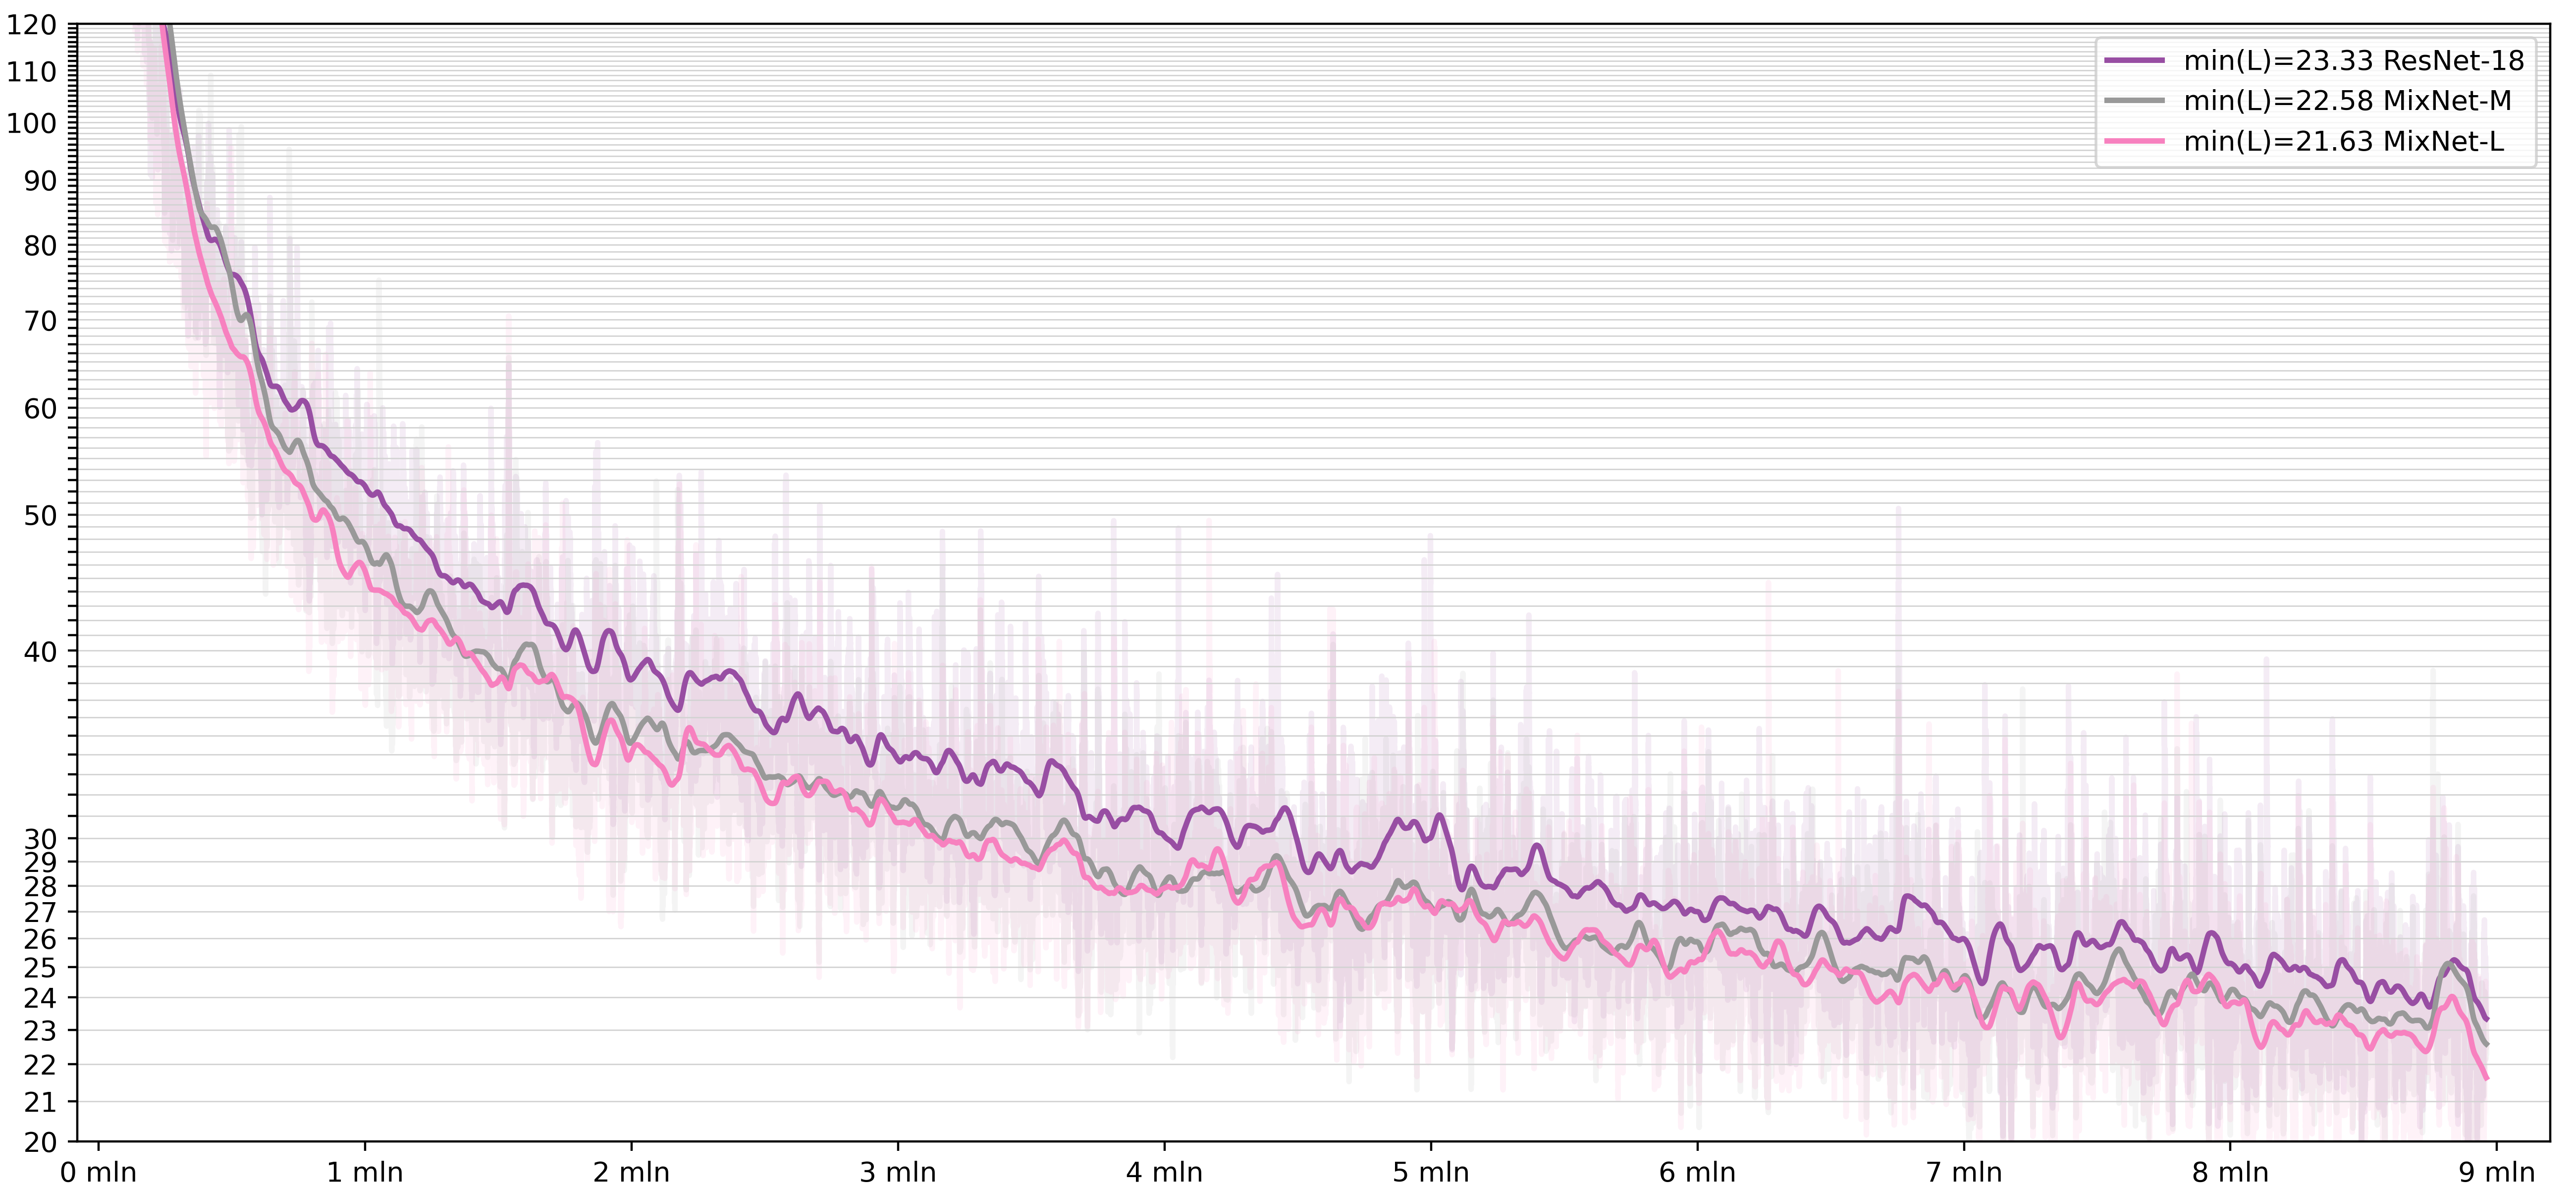
\includegraphics[width=\linewidth]{loss_centerlines_train.png}
    \caption{Wartości funkcji $L$ dla próbek ze zbioru \textbf{treningowego} (wartości najmniejsze podane są dla krzywych uzyskanych z wygładzenia wykładniczego wartości funkcji $L$)}
    \vspace*{1cm}
    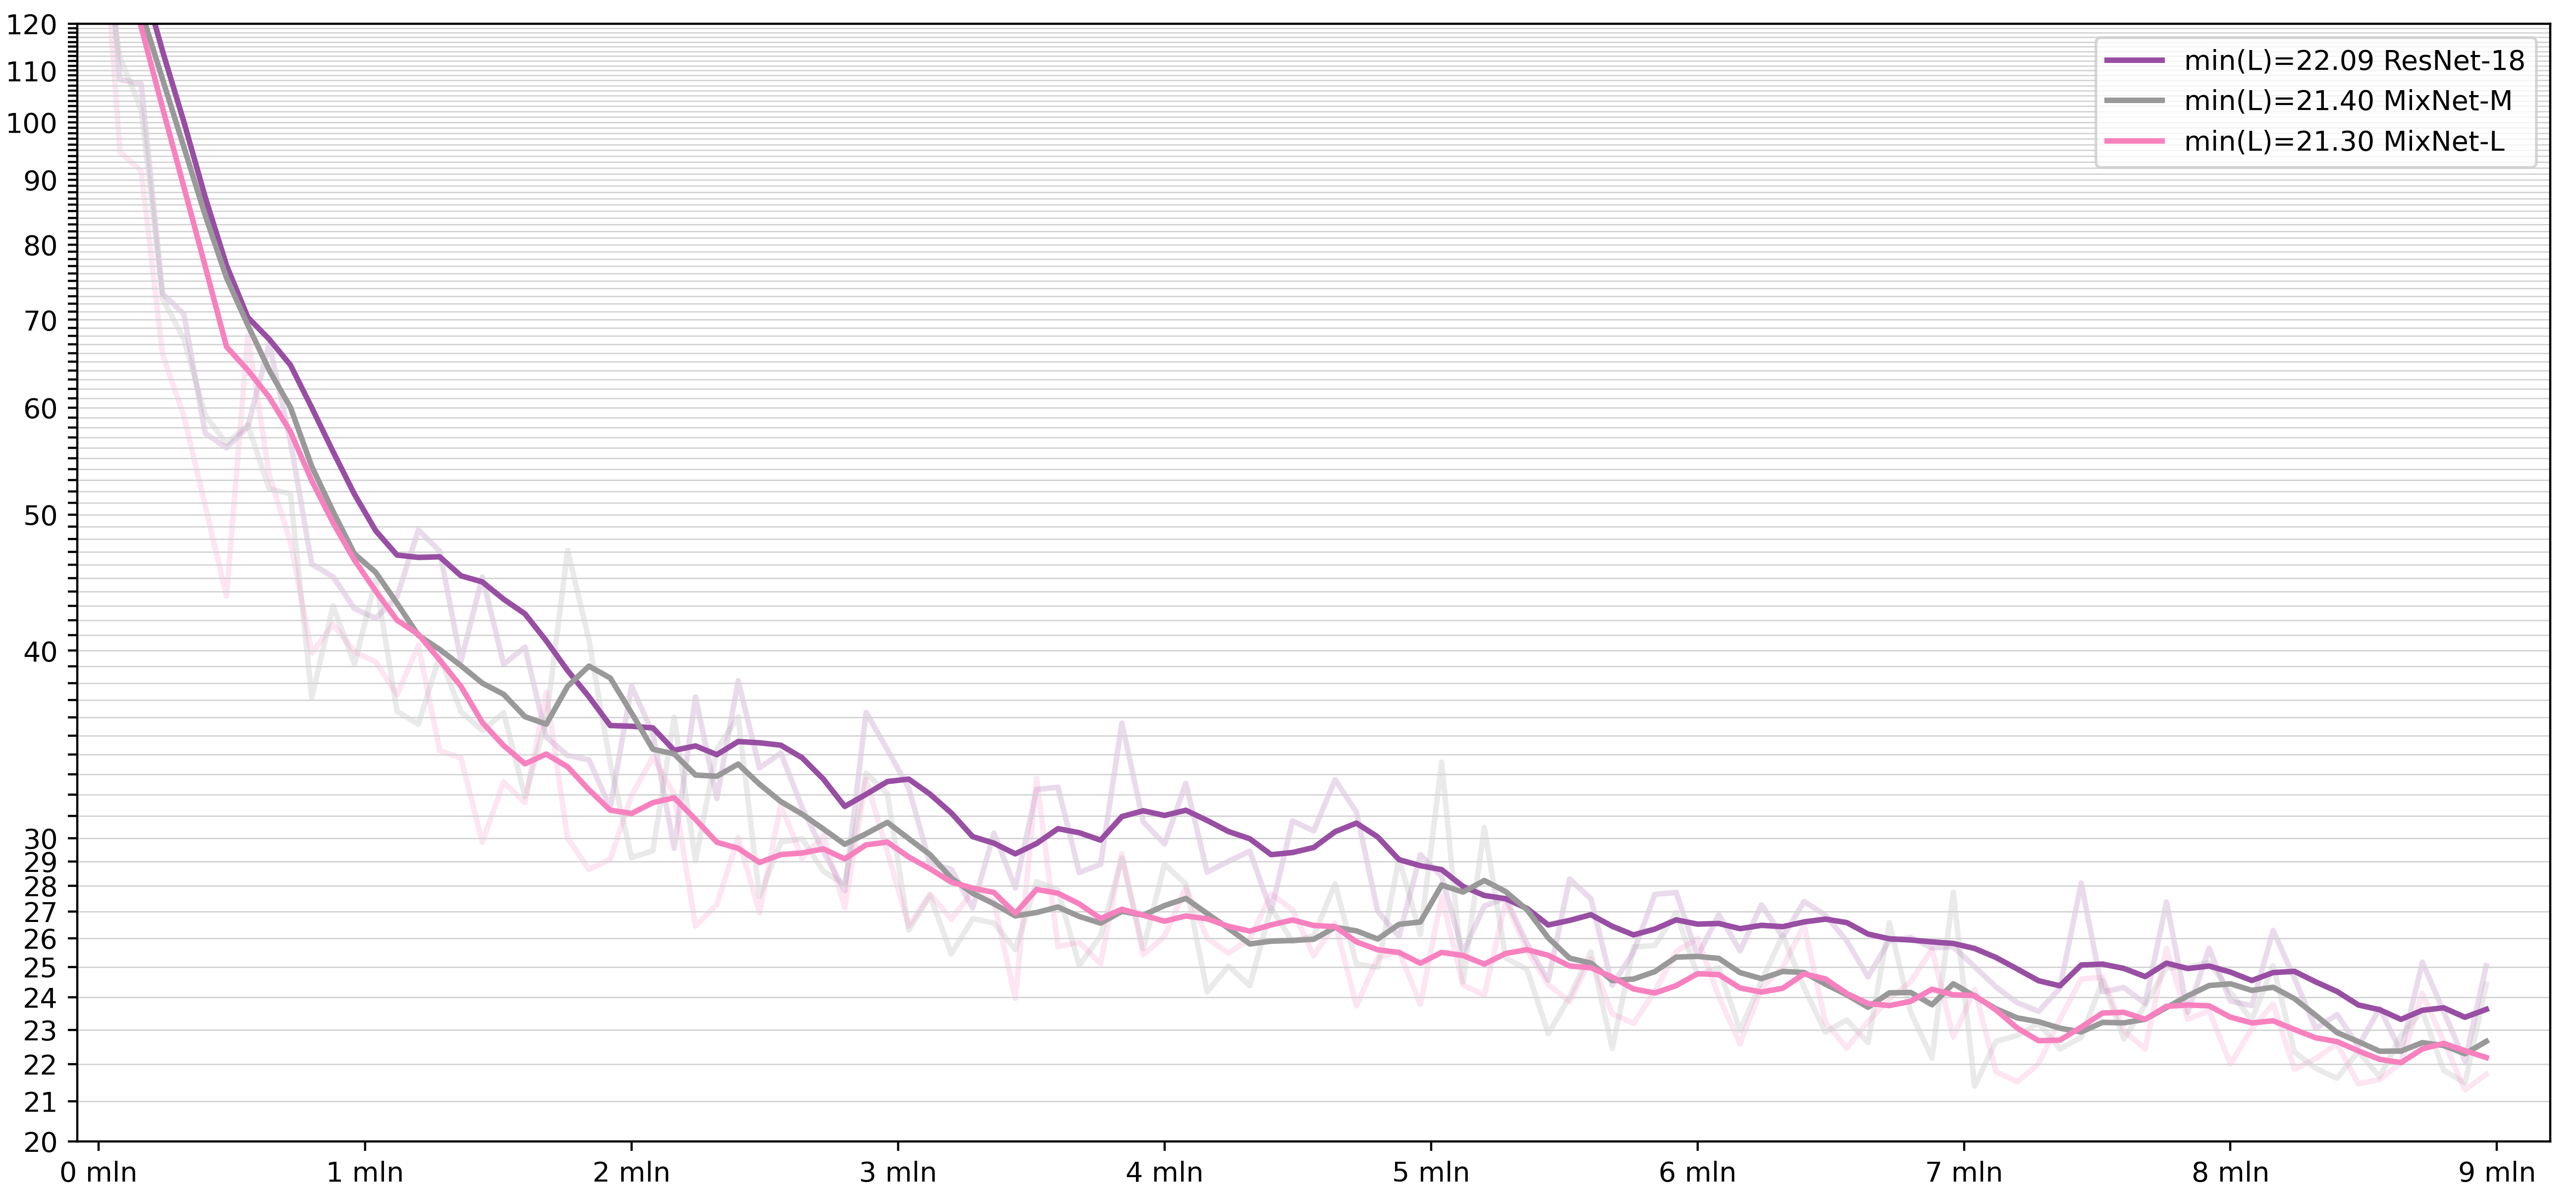
\includegraphics[width=\linewidth]{loss_centerlines_val.png}
    \caption{Wartości funkcji $L$ dla próbek ze zbioru \textbf{walidacyjnego} (wartości najmniejsze podane są dla dokładnych wartości funkcji $L$)}
\end{figure}

\newpage

\section{Opis wizualizacji i wyników}

\subsection{Pierwszy etap}

W pierwszym etapie trenowania, uruchomiono proces dla wszystkich ośmiu sieci neuronowych. Wykonanie jednego cyklu trenowania na pakiecie 16 elementów (ang. batch), zajmowało około 2.18 sekundy. Było to stanowczo za długo, aby przeprowadzić proces trenowania w pełnym zakresie na wszystkich ośmiu sieciach neuronowych. Należy zaznaczyć, że do tak wysokiego czasu cyklu przyczyniły się głównie sieci o dużej liczbie parametrów. Po 465 tys. pakietów (7.44 mln elementów zbioru treningowego), które zostały użyte w procesie trenowania trwającym 12 dni, należało wybrać sieci neuronowe, których trenowanie będzie kontynuowane.

\subsection{Drugi etap}

Wybrano trzy sieci mające najniższe wartości wygładzonej funkcji kosztu na zbiorze walidacyjnym. Były to sieci z następującym szkieletami: \texttt{ResNet-18}, \texttt{MixNet-M}, \texttt{MixNet-L}. Następnie kontynuowano proces trenowania tych trzech sieci. Czas jednego cyklu trenowania zredukowano do 0.44 sekundy. Ten etap trenowania odbył się z wykorzystaniem 1.975 mln pakietów (31.6 mln elementów zbioru treningowego). Etap ten trwał 10 dni.

\subsection{Trzeci etap}

W trzecim etapie przeprowadzono trenowanie wybranych sieci neuronowych z użyciem rasteryzatora \texttt{CenterLines}. Ze względu na ograniczony czas, w którym możliwe byłoby wytrenowanie sieci neuronowych, eksperymenty w trzecim etapie ograniczono do sieci, które wykazały bardzo dobre wyniki z użyciem rasteryzatora \texttt{SemBoxRasterizer} w etapie drugim. Były to sieci o następujących szkieletach: \texttt{ResNet-18}, \texttt{MixNet-M}, \texttt{MixNet-L}. Jeden cykl trenowania trwał 0.53 sekundy. Trenowanie tych sieci trwało 5 dni i odbyło się z wykorzystaniem 560 tys. pakietów (9 mln elementów zbioru treningowego). Wyniki uzyskane z użyciem rasteryzatora \texttt{CenterLines} okazały się gorsze, niż te uzyskane z użyciem rasteryzatora \texttt{SemBoxRasterizer}. Należy mieć na uwadze, że proces trenowania nie został przeprowadzony w pełni (ze względu na ograniczenia czasowe i sprzętowe), możliwe jest, że funkcje kosztu maleją wolniej (z użyciem tego rasteryzatora), ale finalnie osiągnęłyby wartości niższe, niż te uzyskane z rasteryzatorem \texttt{SemBoxRasterizer}. Niestety, aby się o tym przekonać należałoby trenować te 3 sieci przez kolejne kilkadziesiąt dni (do momentu, w którym funkcje kosztu na zbiorze walidacyjnym zaczęłyby rosnąć).
	\cleardoublepage
	
	\chapter{Agregacja modeli}
\thispagestyle{chapterBeginStyle}

\section{Opis problemu}
Predykcja z użyciem jednego modelu jest prosta, model od samego początku jest trenowany pod jedno z góry określone zadanie, w przypadku tej pracy jest to przewidywanie trzech trajektorii z odpowiadającymi prawdopodobieństwami. Problem pojawia się, gdy uzyskuje się kilka niezależnie wytrenowanych modeli predykcyjnych, które posiadają porównywalne skuteczności i nie wiadomo jakimi kryteriami kierować się przy wyborze ostatecznego rozwiązania. W takim scenariuszu najlepsze byłoby użycie pewnej formy głosowania modeli, czyli wykorzystania wiedzy wszystkich dobrze działających modeli do stworzenia jednej predykcji, spójnej z wszystkimi modelami. W przypadku modelowania zmiennej ciągłej (modele regresyjne), można zastosować uśrednianie wyników, w przypadku zmiennych jakościowych (zagadnień klasyfikacyjnych) można zastosować procedurę głosowania, polega ona na wyborze predykcji, która występuje najczęściej. Przy zastosowaniu agregacji modeli można uzyskiwać dokładniejsze i pewniejsze przewidywania. Procedury takie pozwalają również rozwiązać problem naturalnej niestabilności złożonych modeli (poprzez nie wykorzystywanie bezpośrednio predykcji pojedynczych modeli).

\section{Opis użytego rozwiązania}
Charakterystyka predykcji uzyskiwanych przez modele opisane w tej pracy, nie pozwala na zastosowanie uśredniania. Modele zwracają 3 trajektorie, których kolejność nie jest w żaden sposób wymuszona, dodatkowo dwa różne modele mogą zwracać trajektorie które nie są w żaden sposób powiązane (np. opisują 6 różnych odległych trajektorii o małych prawdopodobieństwach realizacji). Do agregacji predykcji modeli został wykorzystany model mieszaniny Gaussa (ten sam, który został wykorzystany do stworzenia równania funkcji kosztu) zaimplementowany jako algorytm \texttt{GMM\_ensemble}. Algorytm wykorzystuje wszystkie trajektorie uzyskane przez sieci neuronowe i dopasowuje do nich trzy trajektorie. Trajektorie uzyskane z agregacji mają również przypisane prawdopodobieństwa realizacji, dzięki temu mogą być wykorzystane do obliczenia funkcji kosztu i porównania takiego podejścia z naiwnym wyborem pojedynczego najlepszego modelu.

\section{Wyniki na zbiorze testowym}
Na zbiorze walidacyjnym zostało zbadane, które sieci neuronowe nadają się do użycia w agregacji. Okazało się, że najlepsza agregacja polega na wykorzystaniu trzech sieci wytrenowanych z użyciem rasteryzatora \texttt{SemBoxRasterizer} o architekturach szkieletu (\texttt{ResNet-18}, \texttt{MixNet-L}, \texttt{MixNet-M}). Wykorzystanie pozostałych sieci jest niewskazane, gdyż zawsze pogarsza wynik agregacji. Poniżej zostały wypisane uśrednione wartości funkcji kosztu na zbiorze testowym. Jak widać żadna pojedyncza sieć nie jest lepsza, niż złożenie składające się z trzech sieci.

\begin{itemize}
    \setlength{\itemsep}{1pt}
    \setlength{\parskip}{0pt}
    \setlength{\parsep}{0pt}
    \item 12.01 - \texttt{ResNet-18}
    \item 11.81 - \texttt{MixNet-L}
    \item 11.74 - \texttt{MixNet-M}
    \item 11.05 - \texttt{GMM\_ensemble(ResNet-18, MixNet-M, MixNet-L)}
\end{itemize}

\newpage
\section{Pseudokod algorytmu \texttt{GMM\_ensemble}}

\begin{pseudokod}[H]
    \SetAlgoLined
    \DontPrintSemicolon
    \textbf{Dane wejściowe:} $models\_preds$\Comment*[r]{Predykcje k modeli (trajektorie i prawdopodobieństwa)}
    
    \BlankLine
    $models\_ens \leftarrow \lbrack \rbrack$\Comment*[r]{Zagregowane predykcje trajektorii i prawdopodobieństw}
    $gmm\_sample\_n \leftarrow 1000$\Comment*[r]{Liczba próbek estymujących rozkład trajektorii}
    
    \BlankLine
    \For{$sample\_pred$ $\in$ $models\_preds$}{
        $mu \leftarrow \lbrack \rbrack$\Comment*[r]{Lista predykcji trajektorii k modeli ($3 \cdot k$ trajektorii)}
        $p \leftarrow \lbrack \rbrack$\Comment*[r]{Lista predykcji prawdopodobieństw k modeli ($3 \cdot k$ prawdopodobieństw)}
        
        \BlankLine
        \For{$model\_pred$ $\in$ $sample\_pred$}{
            $mu.append(model\_pred.trajectories)$\Comment*[r]{3 trajektorie dla każdego modelu}
            $p.append(model\_pred.probabilities)$\Comment*[r]{3 prawdopodobieństwa dla każdego modelu}
        }
        
        \BlankLine
        $p \leftarrow p / sum(p)$\Comment*[r]{Normalizacja, p reprezentuje prawdopodobieństwa realizacji trajektorii}
        $x \leftarrow mu.random\_sample(gmm\_sample\_n, p)$\Comment*[r]{Wybieranie 1000 próbek zgodnie z rozkładem p}
        $x \leftarrow x + random\_normal(\mu=0, \sigma=\epsilon)$\Comment*[r]{Symulowanie próbkowania z mieszaniny rozkładów normalnych}
        
        \BlankLine
        $gm \leftarrow GaussianMixture(n=3).fit(x)$\Comment*[r]{Dopasowanie 3 komponentów do modelu mieszanin Gaussa}
        
        \BlankLine
        $models\_ens.append([gm.means, gm.weights])$\Comment*[r]{Uzyskanie trajektorii i prawdopodobieństw}
    }
    
    \caption{Algorytm GMM\_ensemble}
\end{pseudokod}

\section{Implementacja algorytmu \texttt{GMM\_ensemble}}

\begin{minted}{python}
def GMM_ensemble(pos_arr, conf_arr):
    pos_ens = np.empty(shape=pos_arr.shape[1:])      # agregowane trajektorie
    conf_ens = np.empty(shape=conf_arr.shape[1:])    # agregowane prawdopodobieństwa
    gmm_sample_n = 1000                              # liczba próbek mieszaniny

    for idx in range(pos_arr.shape[1]):
        mu = pos_arr[:, idx, :, :].reshape(-1, 100)  # trajektorie wszystkich modeli
        p = conf_arr[:, idx, :].reshape(-1)          # prawdopodobieństwa modeli
        p = p / p.sum()                              # normalizacja do rozkładu p

        mu_idxs = np.random.choice(                  # wybór próbek do mieszaniny
            mu.shape[0],                             # próbki wybierane z mu
            size=gmm_sample_n,                       # 1000 próbek z powtórzeniami
            p=p                                      # wybrane z rozkładem p
        )
        x = mu[mu_idxs]                              # x to macierz próbek
        x += np.random.normal(                       # wprowadzenie błędów dla lepszej
            loc=0,                                   # zbieżności algorytmu mieszaniny
            scale=0.01,                              # małe zaburzenie, sigma=1cm
            size=(gmm_sample_n, 100)                 # 1000 próbek x 50 pozycji xy
        )
        gm = sklearn.mixture.GaussianMixture(        # rozwiązanie mieszaniny gaussa
            n_components=3,                          # 3 komponenty (trajektorie)
            covariance_type='spherical',             # osobne wariancje dla komponentów
        ).fit(x)                                     # uruchomienie algorytmu na danych x

        pos_ens[idx, :, :], conf_ens[idx, :] = gm.means_, gm.weights_
\end{minted}
	\cleardoublepage
	
	\chapter{Opis ostatecznego rozwiązania}
\thispagestyle{chapterBeginStyle}

\section{Wizualizacja rozwiązania}

\begin{figure}[htbp]
    \centering
    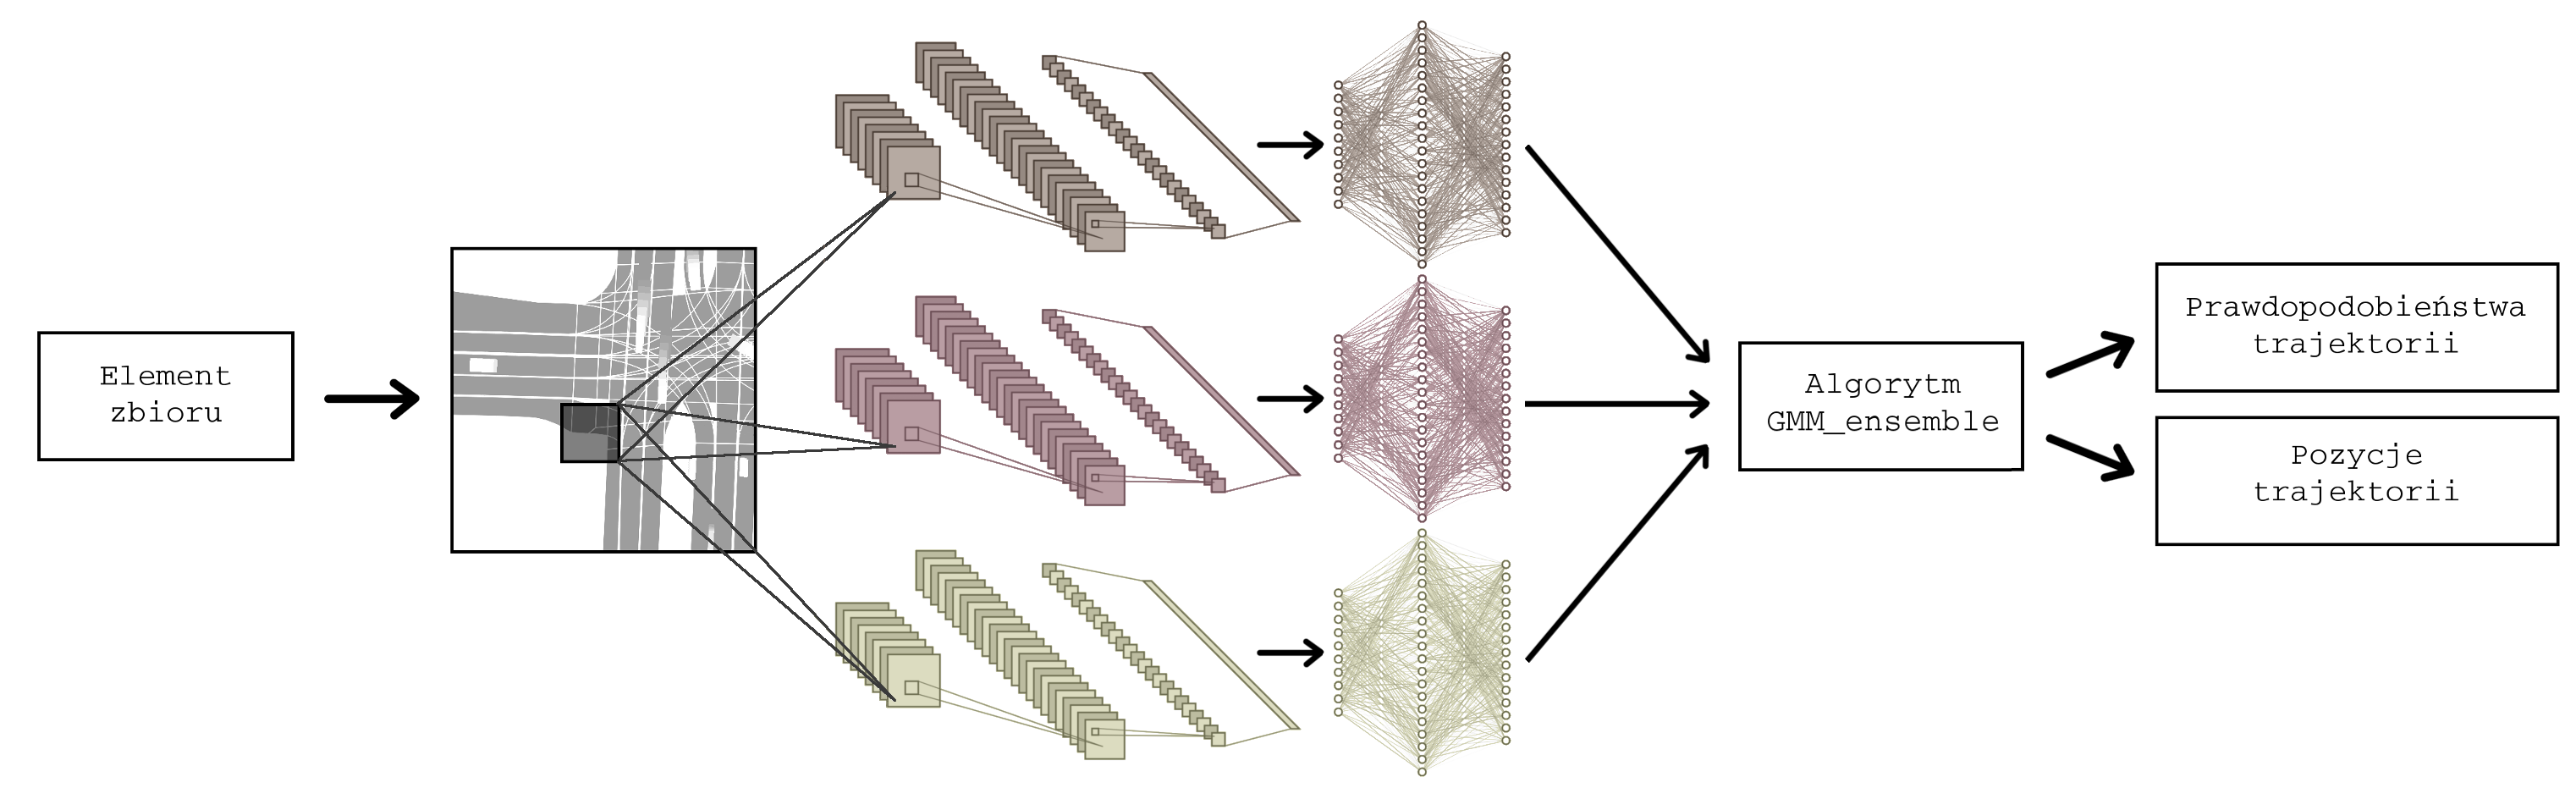
\includegraphics[width=\linewidth]{nn_schema_ensemble.png}
    \caption{Wizualizacja architektury finalnego rozwiązania}
\end{figure}

\section{Opis rozwiązania}
Rozwiązanie, które okazało się najlepsze spośród wszystkich rozważanych w tej pracy to model składający się z trzech sieci neuronowych o architekturach szkieletów \texttt{ResNet-18}, \texttt{MixNet-M}, \texttt{MixNet-L}. Modele te trenowane były z użyciem rasteryzatora \texttt{SemBoxRasterizer} (ten rasteryzator powinien być również wykorzystywany do przewidywania na danych spoza rozważanego zbioru np. w środowisku produkcyjnym). Do agregacji predykcji wykorzystano mieszaninę rozkładów Gaussa, która pozwala na uzyskanie trzech najbardziej prawdopodobnych trajektorii. Model składający się z wcześniej opisanych trzech sieci konwolucyjnych oraz agregacji predykcji posiada uśrednioną wartość funkcji kosztu równą 11.05 (na zbiorze testowym). Jest to bardzo dobry wynik, który można porównać do wartości funkcji kosztu na wizualizacjach w rozdziale 5. Osiągnięty rezultat jest bardzo bliski rozwiązaniom SOTA (ang. state of the art) na wykorzystanym zbiorze danych. Uzyskany model wykorzystuje obliczenia równoległe, dzięki czemu przy wykorzystaniu trzech jednostek GPU, czas jaki jest potrzebny do wykonania predykcji maleje około 3 razy w porównaniu z predykcją na jednej jednostce GPU. Wykonanie jednej predykcji na uzyskanym modelu z trzema jednostkami GPU jest bardzo szybkie, zajmuje około 10ms.
	\cleardoublepage
	
	\chapter{Determinizm procesu trenowania}
\thispagestyle{chapterBeginStyle}

\section{Opis determinizmu}

Algorytm deterministyczny może zostać zdefiniowany poprzez określenie sposobu zmiany stanów maszyny, która wykonuje algorytm. Algorytm jest deterministyczny jeśli dla pewnego stanu i pewnych danych wejściowych istnieje dokładnie jedna dopuszczalna zmiana stanu. W praktyce oznacza to, że zaczynając od pewnego stanu początkowego, można dokładnie określić kolejne stany maszyny wykonującej algorytm.

\section{Determinizm sieci neuronowych}

W kontekście sieci neuronowych, determinizm jest wymagany do zachowania powtarzalności eksperymentów. Posiadając ustalony zbiór treningowy, opis architektury sieci neuronowej oraz algorytm przeprowadzenia procesu trenowania, algorytm powinien za każdym razem zwracać ten sam zbiór parametrów sieci neuronowej. W przypadku trenowania sieci neuronowych na procesorach CPU (ang. central processing unit) wystarczy ustawić wartość ziarna generatora liczb pseudolosowych. Podczas trenowania z użyciem procesora GPU (ang. graphics processing unit), należy wprowadzić kilka dodatkowych zmian, które ograniczają optymalizacje prędkości trenowania, ale zapewniają powtarzalność wyników.

\section{Implementacja determinizmu}
\begin{minted}{python}
import torch                                   # sieci neuronowe
import numpy as np                             # operacje na macierzach
import random                                  # generatory pseudolosowe
import os                                      # modul komunikacji z systemem


def set_seed(seed):
    torch.manual_seed(seed)                    # ustawienie ziarna biblioteki torch
    torch.cuda.manual_seed_all(seed)           # ustawienie ziarna biblioteki cuda
    torch.backends.cudnn.deterministic = True  # deterministyczne algorytmy cudnn
    torch.backends.cudnn.benchmark = False     # stały zbiór algorytmów cudnn
    np.random.seed(seed)                       # ustawienie ziarna biblioteki numpy
    random.seed(seed)                          # ustawienie ziarna biblioteki random
    os.environ['PYTHONHASHSEED'] = str(seed)   # ustawienie ziarna środowiska python


if __name__ == '__main__':
    set_seed(0)                                # ustawienie determinizmu

\end{minted}

\newpage

\section{Dowód obecności determinizmu}

W celu zbadania prawidłowego działania funkcji \texttt{set\_seed} został przeprowadzony eksperyment w którym dwa razy trenowano wcześniej opisywaną sieć neuronową ze szkieletem \texttt{ResNet-18} przez 100 tys. iteracji. Poniżej znajdują się wyniki procesu trenowania. Proces przeprowadzony był tylko aby pokazać determinizm, nie był przeprowadzony w celu radykalnej minimalizacji funkcji kosztu, stąd funkcja kosztu jest dosyć wysoka.

\begin{figure}[htbp]
    \centering
    \subfloat[\centering Pierwszy przebieg trenowania]{{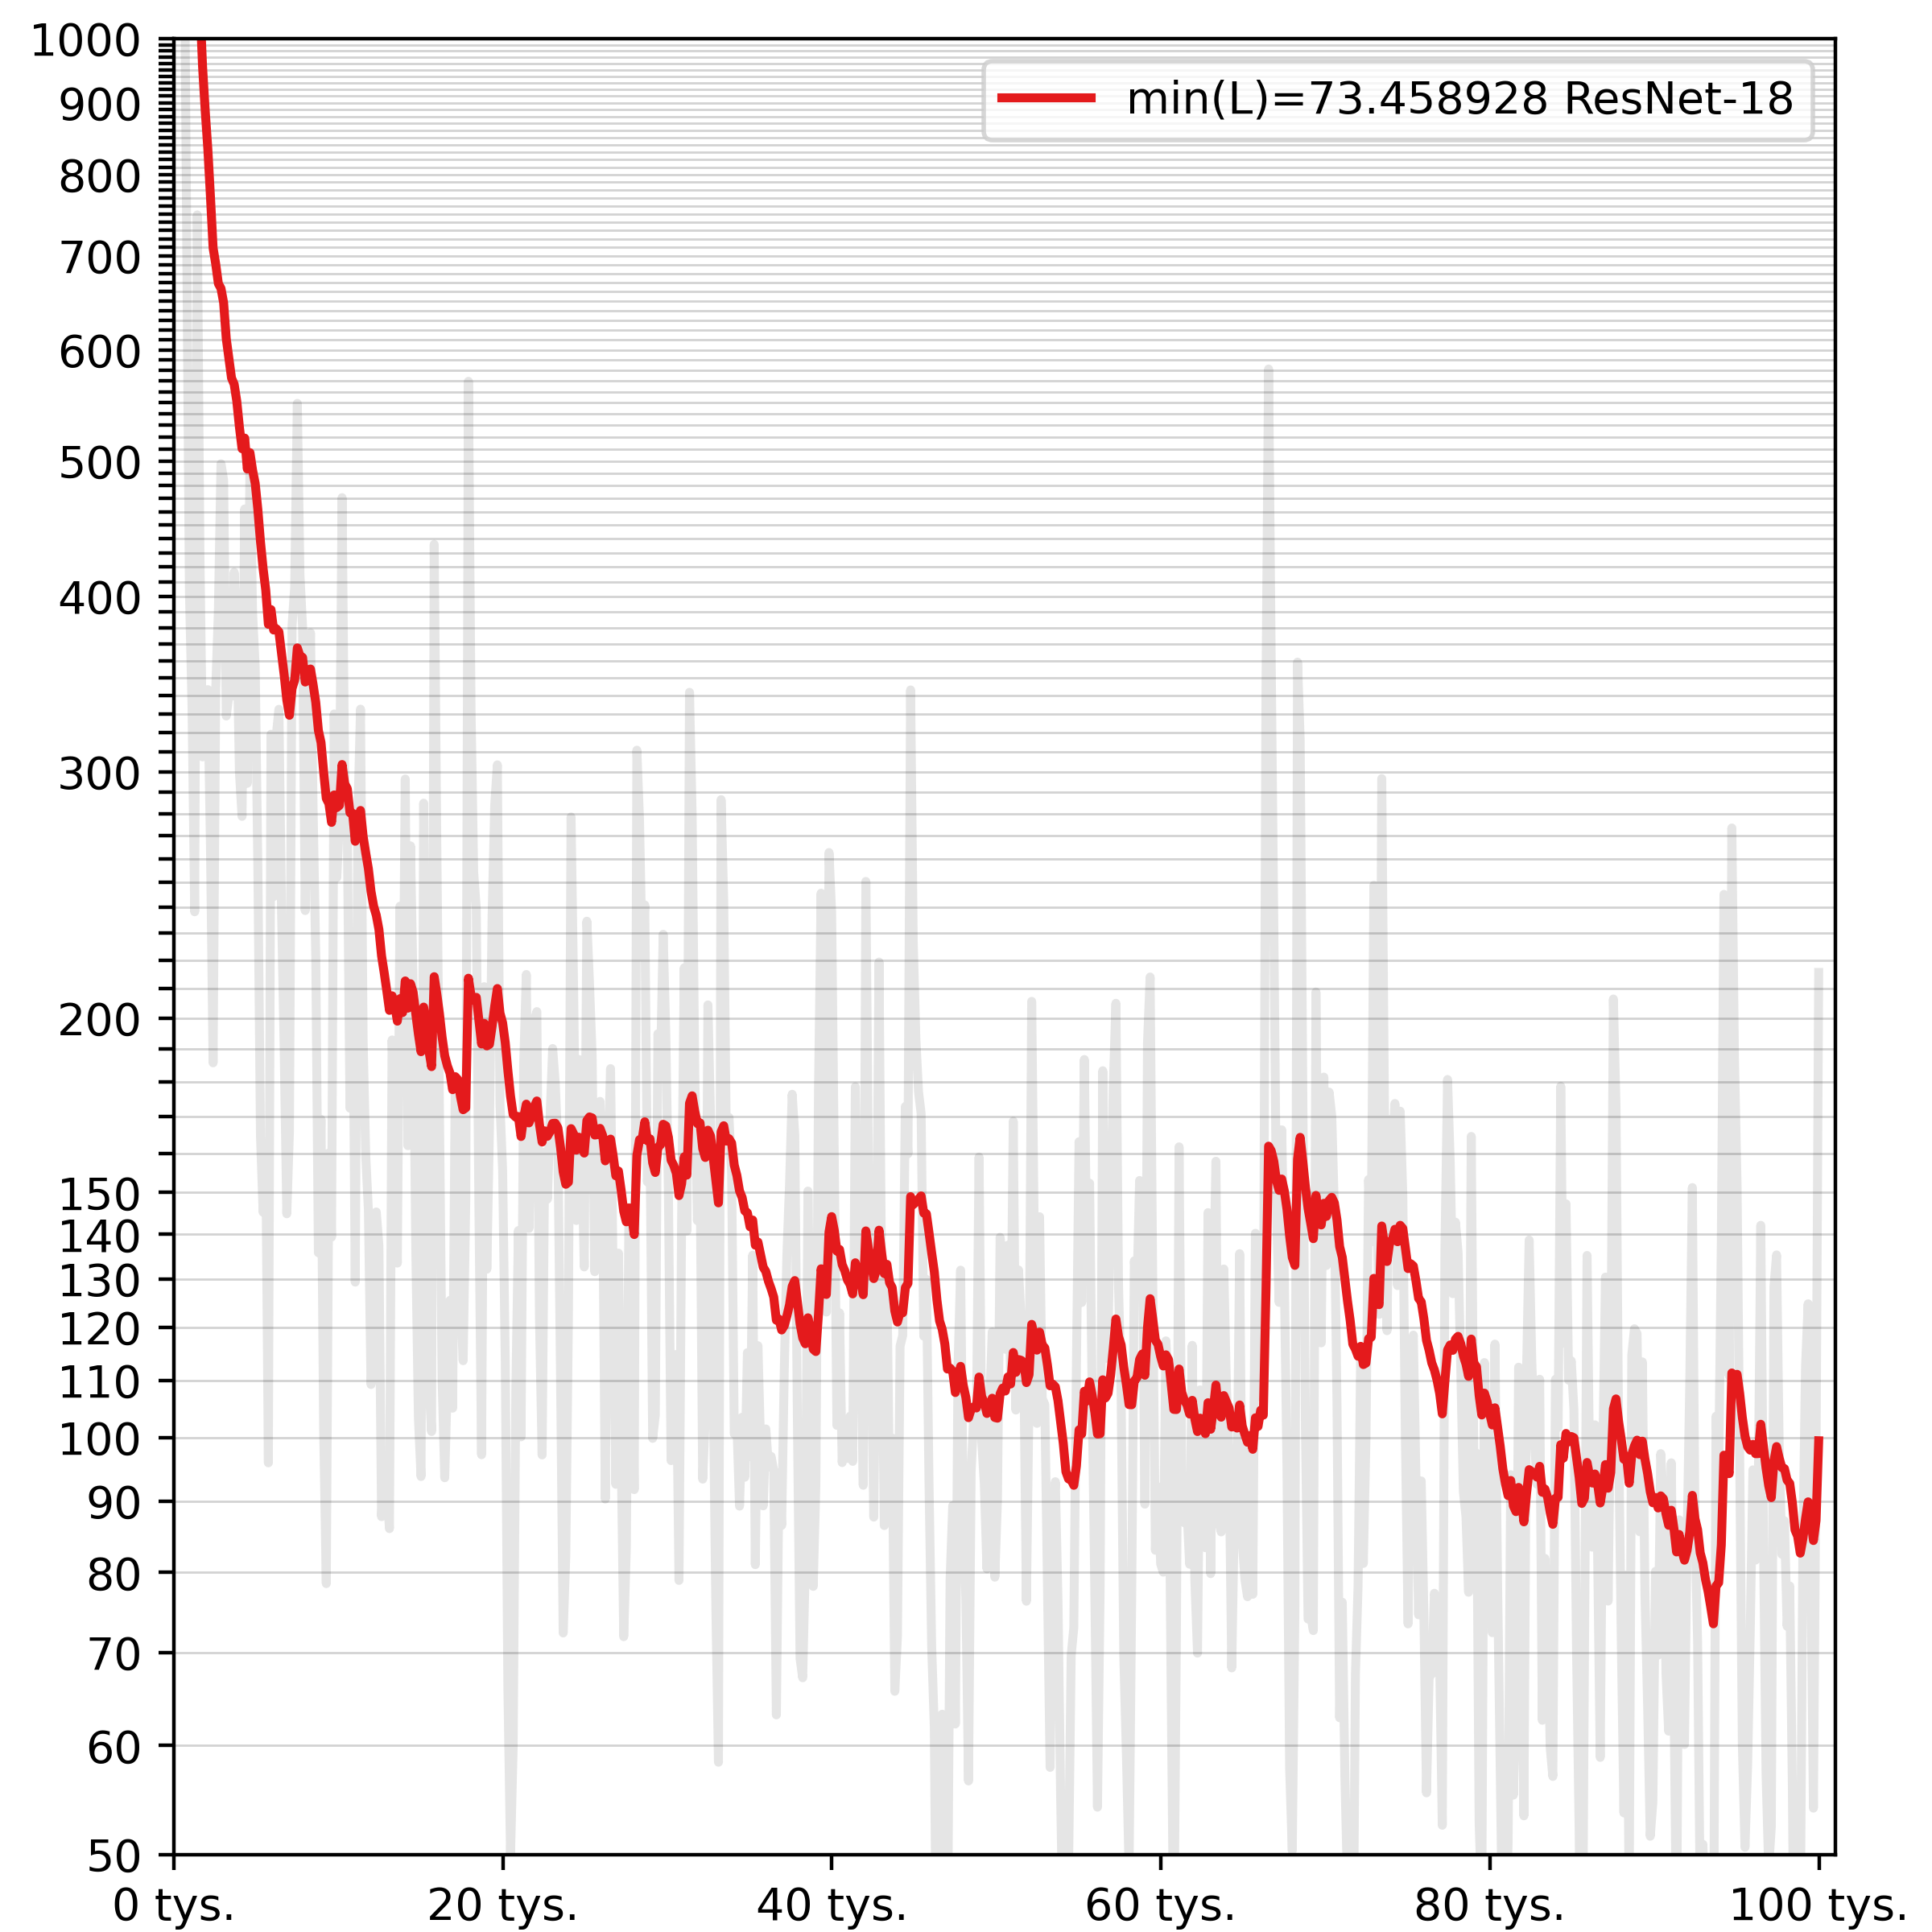
\includegraphics[width=0.47\linewidth]{determinism0.png} }}
    \qquad
    \subfloat[\centering Drugi przebieg trenowania]{{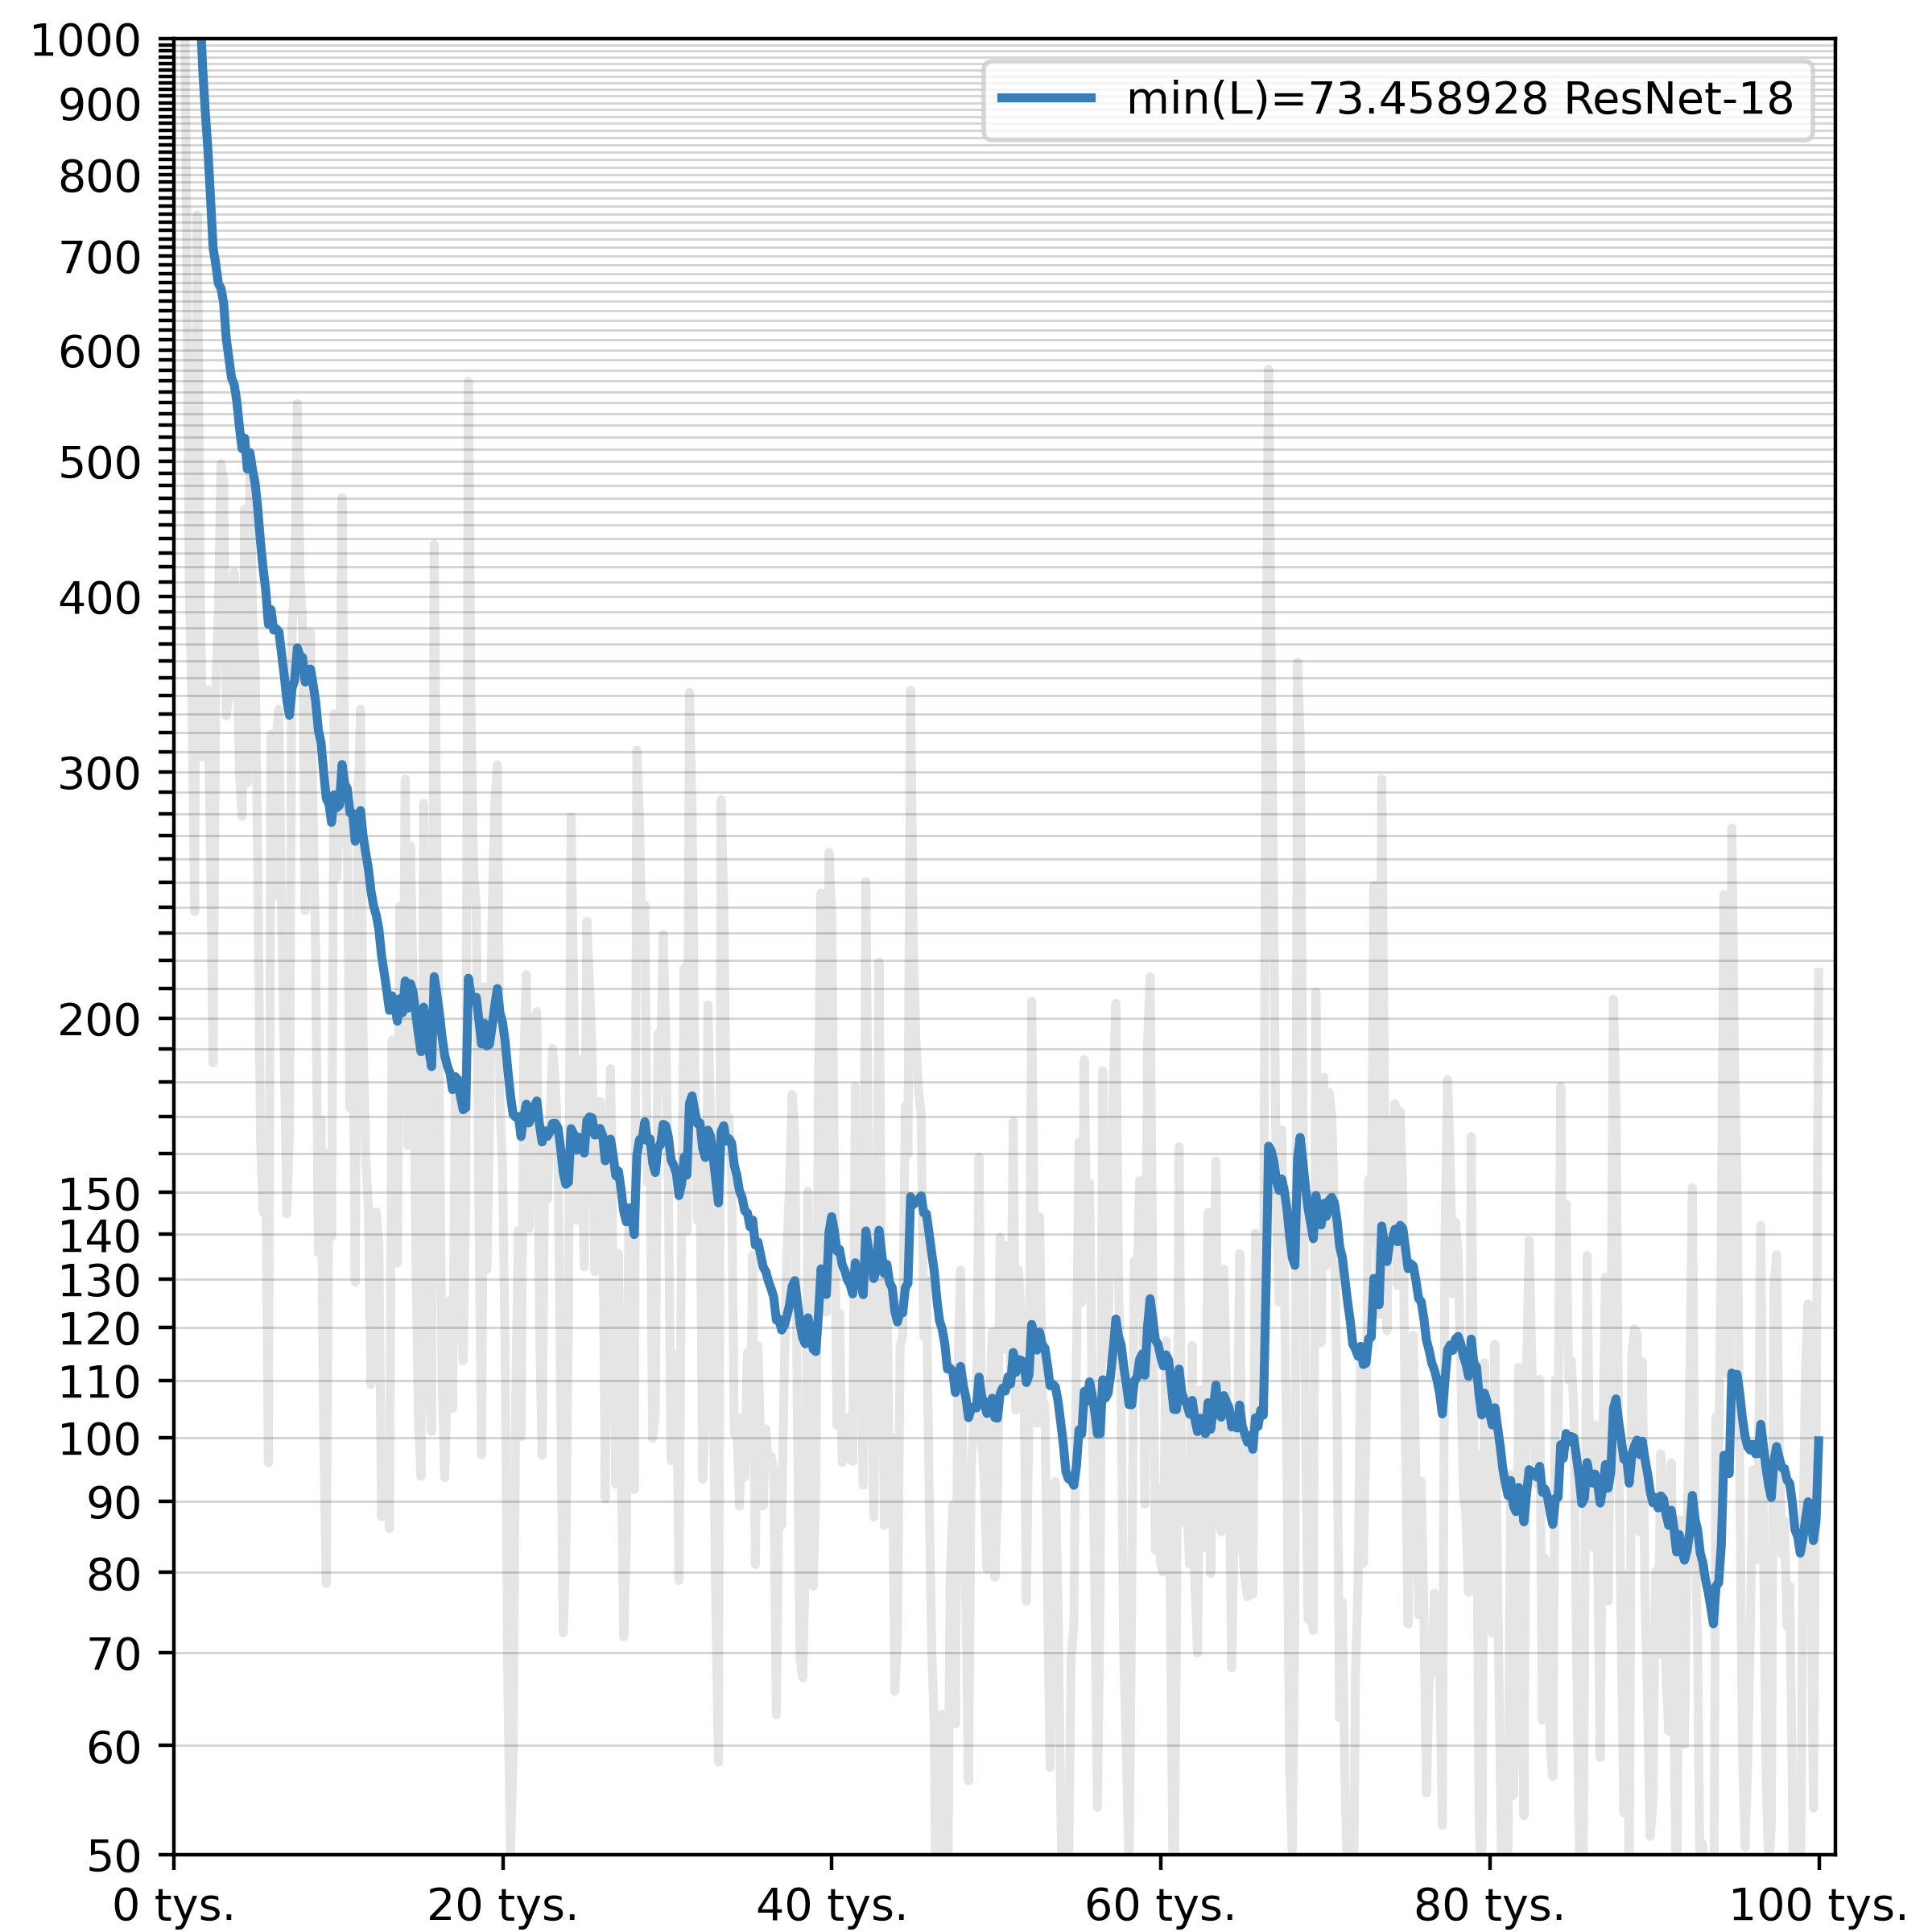
\includegraphics[width=0.47\linewidth]{determinism1.png} }}
\end{figure}

Wyniki uzyskane w dwóch przebiegach algorytmu trenującego są takie same (jak widać na powyższych rysunkach). Wartości funkcji kosztu są identyczne tzn. $|L_0(iter) - L_1(iter)| = 0$. Dowodzi to prawidłowemu działaniu funkcji ustalającej determinizm w procesie trenowania sieci neuronowych.
	\cleardoublepage
	
	\chapter{Podsumowanie}
\thispagestyle{chapterBeginStyle}

Wszystkie etapy pracy inżynierskiej zostały wykonane w pełnym zakresie. Szczegółowo opisano zbiór danych oraz przedstawiono możliwe sposoby jego przetwarzania (rasteryzatory). Znaleziono architekturę sieci neuronowej, która spełnia zadanie predykcji zachowań uczestników ruchu drogowego z bardzo wysoką skutecznością. W pracy zostały opisane eksperymenty, które doprowadziły do uzyskanej architektury. Został omówiony i zaimplementowany nietypowy algorytm agregacji predykcji modeli, który jak się okazało zwiększa skuteczność systemu do poziomu, który nie jest osiągalny za pomocą pojedynczych sieci neuronowych uzyskanych w procesach trenowania.

\vspace{1em}

Należy zaznaczyć, że problem predykcji zachowań uczestników ruchu drogowego jest problemem otwartym, nie istnieje obecnie system, który przewiduje pozycje bezbłędnie. Usprawnienia w rozwiązaniach tego problemu mają na celu nie tylko rozwój nauki, przede wszystkim mają na celu zwiększenie bezpieczeństwa ludzi w środowisku, które w niedalekiej przyszłości może być w dużej mierze zdominowane przez pojazdy autonomiczne. Analiza modeli predykcyjnych opisanych w tej pracy, robiona była z nadzieją, że zwiększy aktualny stan wiedzy na temat systemów predykcyjnych w dziedzinie, która rozwija się bardzo dynamicznie i stanowi bezpośredni czynnik ludzkiego bezpieczeństwa.
	\cleardoublepage
	
	
	%%%%%%%%%%%%%%%%%%%%%%%%%%%%%%%%%%%%%%%%%%%%%%%%%%%%%%%%%%%%%%%%%%%%%%%%%%%%%%
	%%%%%%%%%%%%%%%%%%%%%%%%%%%%%%% BIBLIOGRAFIA %%%%%%%%%%%%%%%%%%%%%%%%%%%%%%%%%
	%%%%%%%%%%%%%%%%%%%%%%%%%%%%%%%%%%%%%%%%%%%%%%%%%%%%%%%%%%%%%%%%%%%%%%%%%%%%%%

	\pagestyle{bibliographyStyle}
	\bibliographystyle{plabbrv}
	\bibliography{literatura}
	\thispagestyle{chapterBeginStyle}
        \addcontentsline{toc}{chapter}{Bibliografia}

	\cleardoublepage
	
	%%%%%%%%%%%%%%%%%%%%%%%%%%%%%%%%%%%%%%%%%%%%%%%%%%%%%%%%%%%%%%%%%%%%%%%%%%%%%%
	%%%%%%%%%%%%%%%%%%%%%%%%%%%%%%%%% DODATKI %%%%%%%%%%%%%%%%%%%%%%%%%%%%%%%%%%%%
	%%%%%%%%%%%%%%%%%%%%%%%%%%%%%%%%%%%%%%%%%%%%%%%%%%%%%%%%%%%%%%%%%%%%%%%%%%%%%%
	
	\appendix
	\pagestyle{appendixStyle}
	
	\chapter{Zawartość płyty CD}
\thispagestyle{chapterBeginStyle}
\label{plytaCD}

\noindent
Płyta CD zawiera trzy katalogi:

\begin{itemize}
    \item \texttt{lyft\_sembox} - Katalog zawiera wszystkie pliki potrzebne do wytrenowania sieci opisanych w tej pracy z użyciem rasteryzatora \texttt{SemBoxRasterizer}.
    \item \texttt{lyft\_centerlines} - Katalog zawiera wszystkie pliki potrzebne do wytrenowania sieci opisanych w tej pracy z użyciem rasteryzatora \texttt{CenterLines}. Katalog zawiera pliki rozpoczynające się prefiksem \texttt{lyft\_mod}, są to pliki, które zawierają zmodyfikowane moduły biblioteki \texttt{l5kit}. Modyfikacje mają za zadanie umożliwienie użycia rasteryzatora \texttt{CenterLines}.
    \item \texttt{analysis} - Katalog zawiera skrypty służące do przeprowadzenia analizy porównawczej sieci neuronowych oraz algorytmu agregacji. Zawiera również skrypty służące do wizualizacji.
\end{itemize}
	\cleardoublepage

\end{document}

